\documentclass[twoside]{book}

% Packages required by doxygen
\usepackage{fixltx2e}
\usepackage{calc}
\usepackage{doxygen}
\usepackage[export]{adjustbox} % also loads graphicx
\usepackage{graphicx}
\usepackage[utf8]{inputenc}
\usepackage{makeidx}
\usepackage{multicol}
\usepackage{multirow}
\PassOptionsToPackage{warn}{textcomp}
\usepackage{textcomp}
\usepackage[nointegrals]{wasysym}
\usepackage[table]{xcolor}

% Font selection
\usepackage[T1]{fontenc}
\usepackage[scaled=.90]{helvet}
\usepackage{courier}
\usepackage{amssymb}
\usepackage{sectsty}
\renewcommand{\familydefault}{\sfdefault}
\allsectionsfont{%
  \fontseries{bc}\selectfont%
  \color{darkgray}%
}
\renewcommand{\DoxyLabelFont}{%
  \fontseries{bc}\selectfont%
  \color{darkgray}%
}
\newcommand{\+}{\discretionary{\mbox{\scriptsize$\hookleftarrow$}}{}{}}

% Page & text layout
\usepackage{geometry}
\geometry{%
  a4paper,%
  top=2.5cm,%
  bottom=2.5cm,%
  left=2.5cm,%
  right=2.5cm%
}
\tolerance=750
\hfuzz=15pt
\hbadness=750
\setlength{\emergencystretch}{15pt}
\setlength{\parindent}{0cm}
\setlength{\parskip}{3ex plus 2ex minus 2ex}
\makeatletter
\renewcommand{\paragraph}{%
  \@startsection{paragraph}{4}{0ex}{-1.0ex}{1.0ex}{%
    \normalfont\normalsize\bfseries\SS@parafont%
  }%
}
\renewcommand{\subparagraph}{%
  \@startsection{subparagraph}{5}{0ex}{-1.0ex}{1.0ex}{%
    \normalfont\normalsize\bfseries\SS@subparafont%
  }%
}
\makeatother

% Headers & footers
\usepackage{fancyhdr}
\pagestyle{fancyplain}
\fancyhead[LE]{\fancyplain{}{\bfseries\thepage}}
\fancyhead[CE]{\fancyplain{}{}}
\fancyhead[RE]{\fancyplain{}{\bfseries\leftmark}}
\fancyhead[LO]{\fancyplain{}{\bfseries\rightmark}}
\fancyhead[CO]{\fancyplain{}{}}
\fancyhead[RO]{\fancyplain{}{\bfseries\thepage}}
\fancyfoot[LE]{\fancyplain{}{}}
\fancyfoot[CE]{\fancyplain{}{}}
\fancyfoot[RE]{\fancyplain{}{\bfseries\scriptsize Generated by Doxygen }}
\fancyfoot[LO]{\fancyplain{}{\bfseries\scriptsize Generated by Doxygen }}
\fancyfoot[CO]{\fancyplain{}{}}
\fancyfoot[RO]{\fancyplain{}{}}
\renewcommand{\footrulewidth}{0.4pt}
\renewcommand{\chaptermark}[1]{%
  \markboth{#1}{}%
}
\renewcommand{\sectionmark}[1]{%
  \markright{\thesection\ #1}%
}

% Indices & bibliography
\usepackage{natbib}
\usepackage[titles]{tocloft}
\setcounter{tocdepth}{3}
\setcounter{secnumdepth}{5}
\makeindex

% Hyperlinks (required, but should be loaded last)
\usepackage{ifpdf}
\ifpdf
  \usepackage[pdftex,pagebackref=true]{hyperref}
\else
  \usepackage[ps2pdf,pagebackref=true]{hyperref}
\fi
\hypersetup{%
  colorlinks=true,%
  linkcolor=blue,%
  citecolor=blue,%
  unicode%
}

% Custom commands
\newcommand{\clearemptydoublepage}{%
  \newpage{\pagestyle{empty}\cleardoublepage}%
}

\usepackage{caption}
\captionsetup{labelsep=space,justification=centering,font={bf},singlelinecheck=off,skip=4pt,position=top}

%===== C O N T E N T S =====

\begin{document}

% Titlepage & ToC
\hypersetup{pageanchor=false,
             bookmarksnumbered=true,
             pdfencoding=unicode
            }
\pagenumbering{alph}
\begin{titlepage}
\vspace*{7cm}
\begin{center}%
{\Large Drider\+Dox \\[1ex]\large 0.\+0 }\\
\vspace*{1cm}
{\large Generated by Doxygen 1.8.13}\\
\end{center}
\end{titlepage}
\clearemptydoublepage
\pagenumbering{roman}
\tableofcontents
\clearemptydoublepage
\pagenumbering{arabic}
\hypersetup{pageanchor=true}

%--- Begin generated contents ---
\chapter{Hierarchical Index}
\section{Class Hierarchy}
This inheritance list is sorted roughly, but not completely, alphabetically\+:\begin{DoxyCompactList}
\item \contentsline{section}{drider\+S\+DK\+:\+:A\+A\+BB}{\pageref{classdrider_s_d_k_1_1_a_a_b_b}}{}
\item \contentsline{section}{drider\+S\+DK\+:\+:Capsule}{\pageref{classdrider_s_d_k_1_1_capsule}}{}
\item \contentsline{section}{drider\+S\+DK\+:\+:Degree}{\pageref{classdrider_s_d_k_1_1_degree}}{}
\item \contentsline{section}{drider\+S\+DK\+:\+:Frustrum}{\pageref{classdrider_s_d_k_1_1_frustrum}}{}
\item \contentsline{section}{drider\+S\+DK\+:\+:Math}{\pageref{structdrider_s_d_k_1_1_math}}{}
\item \contentsline{section}{drider\+S\+DK\+:\+:Matrix3x3}{\pageref{classdrider_s_d_k_1_1_matrix3x3}}{}
\item \contentsline{section}{drider\+S\+DK\+:\+:Matrix4x4}{\pageref{classdrider_s_d_k_1_1_matrix4x4}}{}
\item \contentsline{section}{drider\+S\+DK\+:\+:Matrix\+NxM$<$ \+\_\+rows, \+\_\+cols $>$}{\pageref{classdrider_s_d_k_1_1_matrix_nx_m}}{}
\item \contentsline{section}{drider\+S\+DK\+:\+:Pool$<$ T, pool\+Size $>$}{\pageref{classdrider_s_d_k_1_1_pool}}{}
\item \contentsline{section}{drider\+S\+DK\+:\+:Quaternion}{\pageref{classdrider_s_d_k_1_1_quaternion}}{}
\item \contentsline{section}{drider\+S\+DK\+:\+:Radian}{\pageref{classdrider_s_d_k_1_1_radian}}{}
\item \contentsline{section}{drider\+S\+DK\+:\+:Ray}{\pageref{classdrider_s_d_k_1_1_ray}}{}
\item \contentsline{section}{drider\+S\+DK\+:\+:Sphere}{\pageref{classdrider_s_d_k_1_1_sphere}}{}
\item \contentsline{section}{drider\+S\+DK\+:\+:Vector2D}{\pageref{classdrider_s_d_k_1_1_vector2_d}}{}
\item \contentsline{section}{drider\+S\+DK\+:\+:Vector2\+DI}{\pageref{classdrider_s_d_k_1_1_vector2_d_i}}{}
\item \contentsline{section}{drider\+S\+DK\+:\+:Vector3D}{\pageref{classdrider_s_d_k_1_1_vector3_d}}{}
\begin{DoxyCompactList}
\item \contentsline{section}{drider\+S\+DK\+:\+:Plane}{\pageref{classdrider_s_d_k_1_1_plane}}{}
\end{DoxyCompactList}
\item \contentsline{section}{drider\+S\+DK\+:\+:Vector4D}{\pageref{classdrider_s_d_k_1_1_vector4_d}}{}
\item \contentsline{section}{drider\+S\+DK\+:\+:VectorN$<$ \+\_\+elements $>$}{\pageref{classdrider_s_d_k_1_1_vector_n}}{}
\item \contentsline{section}{drider\+S\+DK\+:\+:Vertex}{\pageref{structdrider_s_d_k_1_1_vertex}}{}
\end{DoxyCompactList}

\chapter{Class Index}
\section{Class List}
Here are the classes, structs, unions and interfaces with brief descriptions\+:\begin{DoxyCompactList}
\item\contentsline{section}{\hyperlink{classdrider_s_d_k_1_1_a_a_b_b}{drider\+S\+D\+K\+::\+A\+A\+BB} }{\pageref{classdrider_s_d_k_1_1_a_a_b_b}}{}
\item\contentsline{section}{\hyperlink{classdrider_s_d_k_1_1_capsule}{drider\+S\+D\+K\+::\+Capsule} }{\pageref{classdrider_s_d_k_1_1_capsule}}{}
\item\contentsline{section}{\hyperlink{classdrider_s_d_k_1_1_degree}{drider\+S\+D\+K\+::\+Degree} }{\pageref{classdrider_s_d_k_1_1_degree}}{}
\item\contentsline{section}{\hyperlink{classdrider_s_d_k_1_1_frustrum}{drider\+S\+D\+K\+::\+Frustrum} }{\pageref{classdrider_s_d_k_1_1_frustrum}}{}
\item\contentsline{section}{\hyperlink{structdrider_s_d_k_1_1_math}{drider\+S\+D\+K\+::\+Math} }{\pageref{structdrider_s_d_k_1_1_math}}{}
\item\contentsline{section}{\hyperlink{classdrider_s_d_k_1_1_matrix3x3}{drider\+S\+D\+K\+::\+Matrix3x3} }{\pageref{classdrider_s_d_k_1_1_matrix3x3}}{}
\item\contentsline{section}{\hyperlink{classdrider_s_d_k_1_1_matrix4x4}{drider\+S\+D\+K\+::\+Matrix4x4} }{\pageref{classdrider_s_d_k_1_1_matrix4x4}}{}
\item\contentsline{section}{\hyperlink{classdrider_s_d_k_1_1_matrix_nx_m}{drider\+S\+D\+K\+::\+Matrix\+Nx\+M$<$ \+\_\+rows, \+\_\+cols $>$} }{\pageref{classdrider_s_d_k_1_1_matrix_nx_m}}{}
\item\contentsline{section}{\hyperlink{classdrider_s_d_k_1_1_plane}{drider\+S\+D\+K\+::\+Plane} }{\pageref{classdrider_s_d_k_1_1_plane}}{}
\item\contentsline{section}{\hyperlink{classdrider_s_d_k_1_1_pool}{drider\+S\+D\+K\+::\+Pool$<$ T, pool\+Size $>$} }{\pageref{classdrider_s_d_k_1_1_pool}}{}
\item\contentsline{section}{\hyperlink{classdrider_s_d_k_1_1_quaternion}{drider\+S\+D\+K\+::\+Quaternion} }{\pageref{classdrider_s_d_k_1_1_quaternion}}{}
\item\contentsline{section}{\hyperlink{classdrider_s_d_k_1_1_radian}{drider\+S\+D\+K\+::\+Radian} }{\pageref{classdrider_s_d_k_1_1_radian}}{}
\item\contentsline{section}{\hyperlink{classdrider_s_d_k_1_1_ray}{drider\+S\+D\+K\+::\+Ray} }{\pageref{classdrider_s_d_k_1_1_ray}}{}
\item\contentsline{section}{\hyperlink{classdrider_s_d_k_1_1_sphere}{drider\+S\+D\+K\+::\+Sphere} }{\pageref{classdrider_s_d_k_1_1_sphere}}{}
\item\contentsline{section}{\hyperlink{classdrider_s_d_k_1_1_vector2_d}{drider\+S\+D\+K\+::\+Vector2D} }{\pageref{classdrider_s_d_k_1_1_vector2_d}}{}
\item\contentsline{section}{\hyperlink{classdrider_s_d_k_1_1_vector2_d_i}{drider\+S\+D\+K\+::\+Vector2\+DI} }{\pageref{classdrider_s_d_k_1_1_vector2_d_i}}{}
\item\contentsline{section}{\hyperlink{classdrider_s_d_k_1_1_vector3_d}{drider\+S\+D\+K\+::\+Vector3D} }{\pageref{classdrider_s_d_k_1_1_vector3_d}}{}
\item\contentsline{section}{\hyperlink{classdrider_s_d_k_1_1_vector4_d}{drider\+S\+D\+K\+::\+Vector4D} }{\pageref{classdrider_s_d_k_1_1_vector4_d}}{}
\item\contentsline{section}{\hyperlink{classdrider_s_d_k_1_1_vector_n}{drider\+S\+D\+K\+::\+Vector\+N$<$ \+\_\+elements $>$} }{\pageref{classdrider_s_d_k_1_1_vector_n}}{}
\item\contentsline{section}{\hyperlink{structdrider_s_d_k_1_1_vertex}{drider\+S\+D\+K\+::\+Vertex} }{\pageref{structdrider_s_d_k_1_1_vertex}}{}
\end{DoxyCompactList}

\chapter{Class Documentation}
\hypertarget{classdrider_s_d_k_1_1_a_a_b_b}{}\section{drider\+S\+DK\+:\+:A\+A\+BB Class Reference}
\label{classdrider_s_d_k_1_1_a_a_b_b}\index{drider\+S\+D\+K\+::\+A\+A\+BB@{drider\+S\+D\+K\+::\+A\+A\+BB}}
\subsection*{Public Member Functions}
\begin{DoxyCompactItemize}
\item 
\hyperlink{classdrider_s_d_k_1_1_a_a_b_b_a290a97c9263d9216f3730c331b24af23}{A\+A\+BB} ()
\item 
\hyperlink{classdrider_s_d_k_1_1_a_a_b_b_a01d474019eb0b1335969de2e36f93fc3}{A\+A\+BB} (float width, float height, const \hyperlink{classdrider_s_d_k_1_1_vector3_d}{Vector3D} \&C)
\item 
\hyperlink{classdrider_s_d_k_1_1_a_a_b_b_a3e8b4fa845074e25f57d0cd6162040db}{A\+A\+BB} (\hyperlink{classdrider_s_d_k_1_1_a_a_b_b}{A\+A\+BB} \&\&A)=default
\item 
\hyperlink{classdrider_s_d_k_1_1_a_a_b_b_a773ae21f2364a88f05338f43c1eda251}{A\+A\+BB} (const \hyperlink{classdrider_s_d_k_1_1_a_a_b_b}{A\+A\+BB} \&A)
\item 
\hyperlink{classdrider_s_d_k_1_1_a_a_b_b_af00f8678f29ff866dde208221f2baf0f}{$\sim$\+A\+A\+BB} ()
\item 
bool \hyperlink{classdrider_s_d_k_1_1_a_a_b_b_aad011cc0c9bafb8fee5e0590935686ab}{intersect} (\hyperlink{classdrider_s_d_k_1_1_a_a_b_b}{A\+A\+BB} \&aabb)
\item 
bool \hyperlink{classdrider_s_d_k_1_1_a_a_b_b_a30da617eda34d0a0396c00cad6bb11fa}{intersect} (\hyperlink{classdrider_s_d_k_1_1_sphere}{Sphere} \&sphere)
\item 
bool \hyperlink{classdrider_s_d_k_1_1_a_a_b_b_af01eb8270121bccab4eb7a891639ba27}{intersect} (\hyperlink{classdrider_s_d_k_1_1_plane}{Plane} \&plane)
\item 
bool \hyperlink{classdrider_s_d_k_1_1_a_a_b_b_a286eedcd8bffca3d22d87f21aab432b1}{intersect} (\hyperlink{classdrider_s_d_k_1_1_frustrum}{Frustrum} \&frustrum)
\item 
bool \hyperlink{classdrider_s_d_k_1_1_a_a_b_b_ad52284fbf96cf41b06d23e05b59df235}{intersect} (\hyperlink{classdrider_s_d_k_1_1_ray}{Ray} \&ray)
\item 
bool \hyperlink{classdrider_s_d_k_1_1_a_a_b_b_a267f402755230b75e2148ea279360593}{intersect} (\hyperlink{classdrider_s_d_k_1_1_vector3_d}{Vector3D} \&point)
\end{DoxyCompactItemize}
\subsection*{Public Attributes}
\begin{DoxyCompactItemize}
\item 
\mbox{\Hypertarget{classdrider_s_d_k_1_1_a_a_b_b_a98cfba128f7bd0c9b22db7c5c8b6da91}\label{classdrider_s_d_k_1_1_a_a_b_b_a98cfba128f7bd0c9b22db7c5c8b6da91}} 
float {\bfseries width}
\item 
\mbox{\Hypertarget{classdrider_s_d_k_1_1_a_a_b_b_aa65615a475c87e4fbe798a6b566c265a}\label{classdrider_s_d_k_1_1_a_a_b_b_aa65615a475c87e4fbe798a6b566c265a}} 
float {\bfseries height}
\item 
\mbox{\Hypertarget{classdrider_s_d_k_1_1_a_a_b_b_a164532986088aef90b04583ba3338d9b}\label{classdrider_s_d_k_1_1_a_a_b_b_a164532986088aef90b04583ba3338d9b}} 
\hyperlink{classdrider_s_d_k_1_1_vector3_d}{Vector3D} {\bfseries center}
\end{DoxyCompactItemize}


\subsection{Constructor \& Destructor Documentation}
\mbox{\Hypertarget{classdrider_s_d_k_1_1_a_a_b_b_a290a97c9263d9216f3730c331b24af23}\label{classdrider_s_d_k_1_1_a_a_b_b_a290a97c9263d9216f3730c331b24af23}} 
\index{drider\+S\+D\+K\+::\+A\+A\+BB@{drider\+S\+D\+K\+::\+A\+A\+BB}!A\+A\+BB@{A\+A\+BB}}
\index{A\+A\+BB@{A\+A\+BB}!drider\+S\+D\+K\+::\+A\+A\+BB@{drider\+S\+D\+K\+::\+A\+A\+BB}}
\subsubsection{\texorpdfstring{A\+A\+B\+B()}{AABB()}\hspace{0.1cm}{\footnotesize\ttfamily [1/4]}}
{\footnotesize\ttfamily drider\+S\+D\+K\+::\+A\+A\+B\+B\+::\+A\+A\+BB (\begin{DoxyParamCaption}{ }\end{DoxyParamCaption})}

Default constructor \mbox{\Hypertarget{classdrider_s_d_k_1_1_a_a_b_b_a01d474019eb0b1335969de2e36f93fc3}\label{classdrider_s_d_k_1_1_a_a_b_b_a01d474019eb0b1335969de2e36f93fc3}} 
\index{drider\+S\+D\+K\+::\+A\+A\+BB@{drider\+S\+D\+K\+::\+A\+A\+BB}!A\+A\+BB@{A\+A\+BB}}
\index{A\+A\+BB@{A\+A\+BB}!drider\+S\+D\+K\+::\+A\+A\+BB@{drider\+S\+D\+K\+::\+A\+A\+BB}}
\subsubsection{\texorpdfstring{A\+A\+B\+B()}{AABB()}\hspace{0.1cm}{\footnotesize\ttfamily [2/4]}}
{\footnotesize\ttfamily drider\+S\+D\+K\+::\+A\+A\+B\+B\+::\+A\+A\+BB (\begin{DoxyParamCaption}\item[{float}]{width,  }\item[{float}]{height,  }\item[{const \hyperlink{classdrider_s_d_k_1_1_vector3_d}{Vector3D} \&}]{C }\end{DoxyParamCaption})}

Initialize the constructor with the given values


\begin{DoxyParams}{Parameters}
{\em s} & Size of the \hyperlink{classdrider_s_d_k_1_1_a_a_b_b}{A\+A\+BB}\\
\hline
{\em C} & Center of the box given by a vector 3D \\
\hline
\end{DoxyParams}
\mbox{\Hypertarget{classdrider_s_d_k_1_1_a_a_b_b_a3e8b4fa845074e25f57d0cd6162040db}\label{classdrider_s_d_k_1_1_a_a_b_b_a3e8b4fa845074e25f57d0cd6162040db}} 
\index{drider\+S\+D\+K\+::\+A\+A\+BB@{drider\+S\+D\+K\+::\+A\+A\+BB}!A\+A\+BB@{A\+A\+BB}}
\index{A\+A\+BB@{A\+A\+BB}!drider\+S\+D\+K\+::\+A\+A\+BB@{drider\+S\+D\+K\+::\+A\+A\+BB}}
\subsubsection{\texorpdfstring{A\+A\+B\+B()}{AABB()}\hspace{0.1cm}{\footnotesize\ttfamily [3/4]}}
{\footnotesize\ttfamily drider\+S\+D\+K\+::\+A\+A\+B\+B\+::\+A\+A\+BB (\begin{DoxyParamCaption}\item[{\hyperlink{classdrider_s_d_k_1_1_a_a_b_b}{A\+A\+BB} \&\&}]{A }\end{DoxyParamCaption})\hspace{0.3cm}{\ttfamily [default]}}

Move constructor. \mbox{\Hypertarget{classdrider_s_d_k_1_1_a_a_b_b_a773ae21f2364a88f05338f43c1eda251}\label{classdrider_s_d_k_1_1_a_a_b_b_a773ae21f2364a88f05338f43c1eda251}} 
\index{drider\+S\+D\+K\+::\+A\+A\+BB@{drider\+S\+D\+K\+::\+A\+A\+BB}!A\+A\+BB@{A\+A\+BB}}
\index{A\+A\+BB@{A\+A\+BB}!drider\+S\+D\+K\+::\+A\+A\+BB@{drider\+S\+D\+K\+::\+A\+A\+BB}}
\subsubsection{\texorpdfstring{A\+A\+B\+B()}{AABB()}\hspace{0.1cm}{\footnotesize\ttfamily [4/4]}}
{\footnotesize\ttfamily drider\+S\+D\+K\+::\+A\+A\+B\+B\+::\+A\+A\+BB (\begin{DoxyParamCaption}\item[{const \hyperlink{classdrider_s_d_k_1_1_a_a_b_b}{A\+A\+BB} \&}]{A }\end{DoxyParamCaption})}

Copy constructor. \mbox{\Hypertarget{classdrider_s_d_k_1_1_a_a_b_b_af00f8678f29ff866dde208221f2baf0f}\label{classdrider_s_d_k_1_1_a_a_b_b_af00f8678f29ff866dde208221f2baf0f}} 
\index{drider\+S\+D\+K\+::\+A\+A\+BB@{drider\+S\+D\+K\+::\+A\+A\+BB}!````~A\+A\+BB@{$\sim$\+A\+A\+BB}}
\index{````~A\+A\+BB@{$\sim$\+A\+A\+BB}!drider\+S\+D\+K\+::\+A\+A\+BB@{drider\+S\+D\+K\+::\+A\+A\+BB}}
\subsubsection{\texorpdfstring{$\sim$\+A\+A\+B\+B()}{~AABB()}}
{\footnotesize\ttfamily drider\+S\+D\+K\+::\+A\+A\+B\+B\+::$\sim$\+A\+A\+BB (\begin{DoxyParamCaption}{ }\end{DoxyParamCaption})}

Default destructor 

\subsection{Member Function Documentation}
\mbox{\Hypertarget{classdrider_s_d_k_1_1_a_a_b_b_aad011cc0c9bafb8fee5e0590935686ab}\label{classdrider_s_d_k_1_1_a_a_b_b_aad011cc0c9bafb8fee5e0590935686ab}} 
\index{drider\+S\+D\+K\+::\+A\+A\+BB@{drider\+S\+D\+K\+::\+A\+A\+BB}!intersect@{intersect}}
\index{intersect@{intersect}!drider\+S\+D\+K\+::\+A\+A\+BB@{drider\+S\+D\+K\+::\+A\+A\+BB}}
\subsubsection{\texorpdfstring{intersect()}{intersect()}\hspace{0.1cm}{\footnotesize\ttfamily [1/6]}}
{\footnotesize\ttfamily bool drider\+S\+D\+K\+::\+A\+A\+B\+B\+::intersect (\begin{DoxyParamCaption}\item[{\hyperlink{classdrider_s_d_k_1_1_a_a_b_b}{A\+A\+BB} \&}]{aabb }\end{DoxyParamCaption})}

Checks for an intersection with another \hyperlink{classdrider_s_d_k_1_1_a_a_b_b}{A\+A\+BB}


\begin{DoxyParams}{Parameters}
{\em aabb} & The other \hyperlink{classdrider_s_d_k_1_1_a_a_b_b}{A\+A\+BB} to check\\
\hline
\end{DoxyParams}
\begin{DoxyReturn}{Returns}
True if it intersects 
\end{DoxyReturn}
\mbox{\Hypertarget{classdrider_s_d_k_1_1_a_a_b_b_a30da617eda34d0a0396c00cad6bb11fa}\label{classdrider_s_d_k_1_1_a_a_b_b_a30da617eda34d0a0396c00cad6bb11fa}} 
\index{drider\+S\+D\+K\+::\+A\+A\+BB@{drider\+S\+D\+K\+::\+A\+A\+BB}!intersect@{intersect}}
\index{intersect@{intersect}!drider\+S\+D\+K\+::\+A\+A\+BB@{drider\+S\+D\+K\+::\+A\+A\+BB}}
\subsubsection{\texorpdfstring{intersect()}{intersect()}\hspace{0.1cm}{\footnotesize\ttfamily [2/6]}}
{\footnotesize\ttfamily bool drider\+S\+D\+K\+::\+A\+A\+B\+B\+::intersect (\begin{DoxyParamCaption}\item[{\hyperlink{classdrider_s_d_k_1_1_sphere}{Sphere} \&}]{sphere }\end{DoxyParamCaption})}

Checks for an intersection with a sphere


\begin{DoxyParams}{Parameters}
{\em sphere} & The sphere to check\\
\hline
\end{DoxyParams}
\begin{DoxyReturn}{Returns}
True if it intersects 
\end{DoxyReturn}
\mbox{\Hypertarget{classdrider_s_d_k_1_1_a_a_b_b_af01eb8270121bccab4eb7a891639ba27}\label{classdrider_s_d_k_1_1_a_a_b_b_af01eb8270121bccab4eb7a891639ba27}} 
\index{drider\+S\+D\+K\+::\+A\+A\+BB@{drider\+S\+D\+K\+::\+A\+A\+BB}!intersect@{intersect}}
\index{intersect@{intersect}!drider\+S\+D\+K\+::\+A\+A\+BB@{drider\+S\+D\+K\+::\+A\+A\+BB}}
\subsubsection{\texorpdfstring{intersect()}{intersect()}\hspace{0.1cm}{\footnotesize\ttfamily [3/6]}}
{\footnotesize\ttfamily bool drider\+S\+D\+K\+::\+A\+A\+B\+B\+::intersect (\begin{DoxyParamCaption}\item[{\hyperlink{classdrider_s_d_k_1_1_plane}{Plane} \&}]{plane }\end{DoxyParamCaption})}

Checks for an intersection with a plane


\begin{DoxyParams}{Parameters}
{\em plane} & The plane to check\\
\hline
\end{DoxyParams}
\begin{DoxyReturn}{Returns}
True if it intersects 
\end{DoxyReturn}
\mbox{\Hypertarget{classdrider_s_d_k_1_1_a_a_b_b_a286eedcd8bffca3d22d87f21aab432b1}\label{classdrider_s_d_k_1_1_a_a_b_b_a286eedcd8bffca3d22d87f21aab432b1}} 
\index{drider\+S\+D\+K\+::\+A\+A\+BB@{drider\+S\+D\+K\+::\+A\+A\+BB}!intersect@{intersect}}
\index{intersect@{intersect}!drider\+S\+D\+K\+::\+A\+A\+BB@{drider\+S\+D\+K\+::\+A\+A\+BB}}
\subsubsection{\texorpdfstring{intersect()}{intersect()}\hspace{0.1cm}{\footnotesize\ttfamily [4/6]}}
{\footnotesize\ttfamily bool drider\+S\+D\+K\+::\+A\+A\+B\+B\+::intersect (\begin{DoxyParamCaption}\item[{\hyperlink{classdrider_s_d_k_1_1_frustrum}{Frustrum} \&}]{frustrum }\end{DoxyParamCaption})}

Checks for an intersection with a frustrum


\begin{DoxyParams}{Parameters}
{\em frustrum} & The frustrum to check\\
\hline
\end{DoxyParams}
\begin{DoxyReturn}{Returns}
True if it intersects 
\end{DoxyReturn}
\mbox{\Hypertarget{classdrider_s_d_k_1_1_a_a_b_b_ad52284fbf96cf41b06d23e05b59df235}\label{classdrider_s_d_k_1_1_a_a_b_b_ad52284fbf96cf41b06d23e05b59df235}} 
\index{drider\+S\+D\+K\+::\+A\+A\+BB@{drider\+S\+D\+K\+::\+A\+A\+BB}!intersect@{intersect}}
\index{intersect@{intersect}!drider\+S\+D\+K\+::\+A\+A\+BB@{drider\+S\+D\+K\+::\+A\+A\+BB}}
\subsubsection{\texorpdfstring{intersect()}{intersect()}\hspace{0.1cm}{\footnotesize\ttfamily [5/6]}}
{\footnotesize\ttfamily bool drider\+S\+D\+K\+::\+A\+A\+B\+B\+::intersect (\begin{DoxyParamCaption}\item[{\hyperlink{classdrider_s_d_k_1_1_ray}{Ray} \&}]{ray }\end{DoxyParamCaption})}

Checks for an intersection with a ray


\begin{DoxyParams}{Parameters}
{\em ray} & The ray to check\\
\hline
\end{DoxyParams}
\begin{DoxyReturn}{Returns}
True if the ray intersects with the \hyperlink{classdrider_s_d_k_1_1_a_a_b_b}{A\+A\+BB} 
\end{DoxyReturn}
\mbox{\Hypertarget{classdrider_s_d_k_1_1_a_a_b_b_a267f402755230b75e2148ea279360593}\label{classdrider_s_d_k_1_1_a_a_b_b_a267f402755230b75e2148ea279360593}} 
\index{drider\+S\+D\+K\+::\+A\+A\+BB@{drider\+S\+D\+K\+::\+A\+A\+BB}!intersect@{intersect}}
\index{intersect@{intersect}!drider\+S\+D\+K\+::\+A\+A\+BB@{drider\+S\+D\+K\+::\+A\+A\+BB}}
\subsubsection{\texorpdfstring{intersect()}{intersect()}\hspace{0.1cm}{\footnotesize\ttfamily [6/6]}}
{\footnotesize\ttfamily bool drider\+S\+D\+K\+::\+A\+A\+B\+B\+::intersect (\begin{DoxyParamCaption}\item[{\hyperlink{classdrider_s_d_k_1_1_vector3_d}{Vector3D} \&}]{point }\end{DoxyParamCaption})}

Checks if the point is in the \hyperlink{classdrider_s_d_k_1_1_a_a_b_b}{A\+A\+BB}


\begin{DoxyParams}{Parameters}
{\em point} & \hyperlink{classdrider_s_d_k_1_1_vector3_d}{Vector3D} that represents the point\\
\hline
\end{DoxyParams}
\begin{DoxyReturn}{Returns}
True if the point is inside 
\end{DoxyReturn}


The documentation for this class was generated from the following files\+:\begin{DoxyCompactItemize}
\item 
C\+:/\+Users/\+Francisco/source/repos/\+Drider-\/\+Engine/\+Math/\+Include/dr\+\_\+aabb.\+h\item 
C\+:/\+Users/\+Francisco/source/repos/\+Drider-\/\+Engine/\+Math/\+Source/dr\+\_\+aabb.\+cpp\end{DoxyCompactItemize}

\hypertarget{classdrider_s_d_k_1_1_capsule}{}\section{drider\+S\+DK\+:\+:Capsule Class Reference}
\label{classdrider_s_d_k_1_1_capsule}\index{drider\+S\+D\+K\+::\+Capsule@{drider\+S\+D\+K\+::\+Capsule}}
\subsection*{Public Attributes}
\begin{DoxyCompactItemize}
\item 
\mbox{\Hypertarget{classdrider_s_d_k_1_1_capsule_ace6d0e6c5710041739e7700c36b47252}\label{classdrider_s_d_k_1_1_capsule_ace6d0e6c5710041739e7700c36b47252}} 
\hyperlink{classdrider_s_d_k_1_1_vector3_d}{Vector3D} {\bfseries pointA}
\item 
\mbox{\Hypertarget{classdrider_s_d_k_1_1_capsule_ab803c439dbf76b119206737c18ca9ebe}\label{classdrider_s_d_k_1_1_capsule_ab803c439dbf76b119206737c18ca9ebe}} 
\hyperlink{classdrider_s_d_k_1_1_vector3_d}{Vector3D} {\bfseries pointB}
\item 
\mbox{\Hypertarget{classdrider_s_d_k_1_1_capsule_a7c669246aed67d96f518f92f633a0883}\label{classdrider_s_d_k_1_1_capsule_a7c669246aed67d96f518f92f633a0883}} 
float {\bfseries radio}
\end{DoxyCompactItemize}


The documentation for this class was generated from the following file\+:\begin{DoxyCompactItemize}
\item 
C\+:/\+Users/\+Francisco/source/repos/\+Drider-\/\+Engine/\+Math/\+Include/dr\+\_\+capsule.\+h\end{DoxyCompactItemize}

\hypertarget{classdrider_s_d_k_1_1_degree}{}\section{drider\+S\+DK\+:\+:Degree Class Reference}
\label{classdrider_s_d_k_1_1_degree}\index{drider\+S\+D\+K\+::\+Degree@{drider\+S\+D\+K\+::\+Degree}}
\subsection*{Public Member Functions}
\begin{DoxyCompactItemize}
\item 
\hyperlink{classdrider_s_d_k_1_1_degree_aa02a04e5e7f0c5d15e4362bfc2022286}{Degree} ()
\item 
\hyperlink{classdrider_s_d_k_1_1_degree_ab8798b0761abe03fd0d28abbac62a17c}{Degree} (\hyperlink{classdrider_s_d_k_1_1_degree}{Degree} \&\&V)=default
\item 
\hyperlink{classdrider_s_d_k_1_1_degree_a94a3842a811edb51f578d4f6da487e3b}{Degree} (const \hyperlink{classdrider_s_d_k_1_1_degree}{Degree} \&V)
\item 
\hyperlink{classdrider_s_d_k_1_1_degree_ada0c9ad7f00c36d1209fc1e7794911d7}{Degree} (float value)
\item 
\hyperlink{classdrider_s_d_k_1_1_degree_a44a8904fbd4178de2916c2b54883c1e1}{$\sim$\+Degree} ()
\item 
float \hyperlink{classdrider_s_d_k_1_1_degree_a5904a76d6c28c10ca432ee46db1997a8}{to\+Radian} () const
\item 
\hyperlink{classdrider_s_d_k_1_1_degree}{Degree} \& \hyperlink{classdrider_s_d_k_1_1_degree_a1dedd27ddf700baf9c6f706888e81d0a}{to\+Range} ()
\item 
\mbox{\Hypertarget{classdrider_s_d_k_1_1_degree_abf1e9a263d6e3acaebd79f1f1f6e4791}\label{classdrider_s_d_k_1_1_degree_abf1e9a263d6e3acaebd79f1f1f6e4791}} 
{\bfseries operator float} ()
\item 
\mbox{\Hypertarget{classdrider_s_d_k_1_1_degree_a4320abb846750e3ea3de34895e56dc03}\label{classdrider_s_d_k_1_1_degree_a4320abb846750e3ea3de34895e56dc03}} 
\hyperlink{classdrider_s_d_k_1_1_degree}{Degree} \& {\bfseries operator=} (float V)
\item 
\mbox{\Hypertarget{classdrider_s_d_k_1_1_degree_a06e5895da5d163da2753a7f05f3e3e56}\label{classdrider_s_d_k_1_1_degree_a06e5895da5d163da2753a7f05f3e3e56}} 
\hyperlink{classdrider_s_d_k_1_1_degree}{Degree} \& {\bfseries operator+=} (float V)
\item 
\mbox{\Hypertarget{classdrider_s_d_k_1_1_degree_a89b96313fb2d245b326378985d887aff}\label{classdrider_s_d_k_1_1_degree_a89b96313fb2d245b326378985d887aff}} 
\hyperlink{classdrider_s_d_k_1_1_degree}{Degree} \& {\bfseries operator-\/=} (float V)
\item 
\mbox{\Hypertarget{classdrider_s_d_k_1_1_degree_a61bca4212d64c8676f6fd39956df7e3e}\label{classdrider_s_d_k_1_1_degree_a61bca4212d64c8676f6fd39956df7e3e}} 
\hyperlink{classdrider_s_d_k_1_1_degree}{Degree} \& {\bfseries operator$\ast$=} (float V)
\item 
\mbox{\Hypertarget{classdrider_s_d_k_1_1_degree_a13d3186e5c614087168767a9090c501e}\label{classdrider_s_d_k_1_1_degree_a13d3186e5c614087168767a9090c501e}} 
\hyperlink{classdrider_s_d_k_1_1_degree}{Degree} \& {\bfseries operator/=} (float V)
\end{DoxyCompactItemize}
\subsection*{Private Attributes}
\begin{DoxyCompactItemize}
\item 
\mbox{\Hypertarget{classdrider_s_d_k_1_1_degree_abdb67b756d1b1889833b05019b56f1d1}\label{classdrider_s_d_k_1_1_degree_abdb67b756d1b1889833b05019b56f1d1}} 
float {\bfseries m\+\_\+value}
\end{DoxyCompactItemize}


\subsection{Constructor \& Destructor Documentation}
\mbox{\Hypertarget{classdrider_s_d_k_1_1_degree_aa02a04e5e7f0c5d15e4362bfc2022286}\label{classdrider_s_d_k_1_1_degree_aa02a04e5e7f0c5d15e4362bfc2022286}} 
\index{drider\+S\+D\+K\+::\+Degree@{drider\+S\+D\+K\+::\+Degree}!Degree@{Degree}}
\index{Degree@{Degree}!drider\+S\+D\+K\+::\+Degree@{drider\+S\+D\+K\+::\+Degree}}
\subsubsection{\texorpdfstring{Degree()}{Degree()}\hspace{0.1cm}{\footnotesize\ttfamily [1/4]}}
{\footnotesize\ttfamily drider\+S\+D\+K\+::\+Degree\+::\+Degree (\begin{DoxyParamCaption}{ }\end{DoxyParamCaption})}

Default constructor. \mbox{\Hypertarget{classdrider_s_d_k_1_1_degree_ab8798b0761abe03fd0d28abbac62a17c}\label{classdrider_s_d_k_1_1_degree_ab8798b0761abe03fd0d28abbac62a17c}} 
\index{drider\+S\+D\+K\+::\+Degree@{drider\+S\+D\+K\+::\+Degree}!Degree@{Degree}}
\index{Degree@{Degree}!drider\+S\+D\+K\+::\+Degree@{drider\+S\+D\+K\+::\+Degree}}
\subsubsection{\texorpdfstring{Degree()}{Degree()}\hspace{0.1cm}{\footnotesize\ttfamily [2/4]}}
{\footnotesize\ttfamily drider\+S\+D\+K\+::\+Degree\+::\+Degree (\begin{DoxyParamCaption}\item[{\hyperlink{classdrider_s_d_k_1_1_degree}{Degree} \&\&}]{V }\end{DoxyParamCaption})\hspace{0.3cm}{\ttfamily [default]}}

Move constructor. \mbox{\Hypertarget{classdrider_s_d_k_1_1_degree_a94a3842a811edb51f578d4f6da487e3b}\label{classdrider_s_d_k_1_1_degree_a94a3842a811edb51f578d4f6da487e3b}} 
\index{drider\+S\+D\+K\+::\+Degree@{drider\+S\+D\+K\+::\+Degree}!Degree@{Degree}}
\index{Degree@{Degree}!drider\+S\+D\+K\+::\+Degree@{drider\+S\+D\+K\+::\+Degree}}
\subsubsection{\texorpdfstring{Degree()}{Degree()}\hspace{0.1cm}{\footnotesize\ttfamily [3/4]}}
{\footnotesize\ttfamily drider\+S\+D\+K\+::\+Degree\+::\+Degree (\begin{DoxyParamCaption}\item[{const \hyperlink{classdrider_s_d_k_1_1_degree}{Degree} \&}]{V }\end{DoxyParamCaption})}

Copy constructor. \mbox{\Hypertarget{classdrider_s_d_k_1_1_degree_ada0c9ad7f00c36d1209fc1e7794911d7}\label{classdrider_s_d_k_1_1_degree_ada0c9ad7f00c36d1209fc1e7794911d7}} 
\index{drider\+S\+D\+K\+::\+Degree@{drider\+S\+D\+K\+::\+Degree}!Degree@{Degree}}
\index{Degree@{Degree}!drider\+S\+D\+K\+::\+Degree@{drider\+S\+D\+K\+::\+Degree}}
\subsubsection{\texorpdfstring{Degree()}{Degree()}\hspace{0.1cm}{\footnotesize\ttfamily [4/4]}}
{\footnotesize\ttfamily drider\+S\+D\+K\+::\+Degree\+::\+Degree (\begin{DoxyParamCaption}\item[{float}]{value }\end{DoxyParamCaption})\hspace{0.3cm}{\ttfamily [explicit]}}

Initialize class with value.


\begin{DoxyParams}{Parameters}
{\em value} & Initial value of the class. \\
\hline
\end{DoxyParams}
\mbox{\Hypertarget{classdrider_s_d_k_1_1_degree_a44a8904fbd4178de2916c2b54883c1e1}\label{classdrider_s_d_k_1_1_degree_a44a8904fbd4178de2916c2b54883c1e1}} 
\index{drider\+S\+D\+K\+::\+Degree@{drider\+S\+D\+K\+::\+Degree}!````~Degree@{$\sim$\+Degree}}
\index{````~Degree@{$\sim$\+Degree}!drider\+S\+D\+K\+::\+Degree@{drider\+S\+D\+K\+::\+Degree}}
\subsubsection{\texorpdfstring{$\sim$\+Degree()}{~Degree()}}
{\footnotesize\ttfamily drider\+S\+D\+K\+::\+Degree\+::$\sim$\+Degree (\begin{DoxyParamCaption}{ }\end{DoxyParamCaption})}

Default destructor. 

\subsection{Member Function Documentation}
\mbox{\Hypertarget{classdrider_s_d_k_1_1_degree_a5904a76d6c28c10ca432ee46db1997a8}\label{classdrider_s_d_k_1_1_degree_a5904a76d6c28c10ca432ee46db1997a8}} 
\index{drider\+S\+D\+K\+::\+Degree@{drider\+S\+D\+K\+::\+Degree}!to\+Radian@{to\+Radian}}
\index{to\+Radian@{to\+Radian}!drider\+S\+D\+K\+::\+Degree@{drider\+S\+D\+K\+::\+Degree}}
\subsubsection{\texorpdfstring{to\+Radian()}{toRadian()}}
{\footnotesize\ttfamily float drider\+S\+D\+K\+::\+Degree\+::to\+Radian (\begin{DoxyParamCaption}{ }\end{DoxyParamCaption}) const}

Returns a \hyperlink{classdrider_s_d_k_1_1_radian}{Radian} class with a value equal to the actual degrees in radians.

\begin{DoxyReturn}{Returns}
Class radian. 
\end{DoxyReturn}
\mbox{\Hypertarget{classdrider_s_d_k_1_1_degree_a1dedd27ddf700baf9c6f706888e81d0a}\label{classdrider_s_d_k_1_1_degree_a1dedd27ddf700baf9c6f706888e81d0a}} 
\index{drider\+S\+D\+K\+::\+Degree@{drider\+S\+D\+K\+::\+Degree}!to\+Range@{to\+Range}}
\index{to\+Range@{to\+Range}!drider\+S\+D\+K\+::\+Degree@{drider\+S\+D\+K\+::\+Degree}}
\subsubsection{\texorpdfstring{to\+Range()}{toRange()}}
{\footnotesize\ttfamily \hyperlink{classdrider_s_d_k_1_1_degree}{Degree} \& drider\+S\+D\+K\+::\+Degree\+::to\+Range (\begin{DoxyParamCaption}{ }\end{DoxyParamCaption})}

Limit the value in \mbox{[}0, 360)

\begin{DoxyReturn}{Returns}
A reference to this class. 
\end{DoxyReturn}


The documentation for this class was generated from the following files\+:\begin{DoxyCompactItemize}
\item 
C\+:/\+Users/\+Francisco/source/repos/\+Drider-\/\+Engine/\+Math/\+Include/dr\+\_\+degree.\+h\item 
C\+:/\+Users/\+Francisco/source/repos/\+Drider-\/\+Engine/\+Math/\+Source/dr\+\_\+degree.\+cpp\end{DoxyCompactItemize}

\hypertarget{classdrider_s_d_k_1_1_frustrum}{}\section{drider\+S\+DK\+:\+:Frustrum Class Reference}
\label{classdrider_s_d_k_1_1_frustrum}\index{drider\+S\+D\+K\+::\+Frustrum@{drider\+S\+D\+K\+::\+Frustrum}}
\subsection*{Public Types}
\begin{DoxyCompactItemize}
\item 
\mbox{\Hypertarget{classdrider_s_d_k_1_1_frustrum_afb452e1845d8d057840dec11ad282f0a}\label{classdrider_s_d_k_1_1_frustrum_afb452e1845d8d057840dec11ad282f0a}} 
enum {\bfseries P\+L\+A\+N\+ES} \{ \newline
{\bfseries k\+Left}, 
{\bfseries k\+Right}, 
{\bfseries k\+Top}, 
{\bfseries k\+Bottom}, 
\newline
{\bfseries k\+Near}, 
{\bfseries k\+Far}
 \}
\end{DoxyCompactItemize}
\subsection*{Public Member Functions}
\begin{DoxyCompactItemize}
\item 
\hyperlink{classdrider_s_d_k_1_1_frustrum_a4a79e8234bbf25c8cf850f01a6485a1a}{Frustrum} (const \hyperlink{classdrider_s_d_k_1_1_matrix4x4}{Matrix4x4} \&View\+Projection)
\item 
void \hyperlink{classdrider_s_d_k_1_1_frustrum_a852e86146dc8621a99c5581e03d587de}{create\+From\+VP} (const \hyperlink{classdrider_s_d_k_1_1_matrix4x4}{Matrix4x4} \&View\+Projection)
\item 
bool \hyperlink{classdrider_s_d_k_1_1_frustrum_ad81116f896faad5acada10c16c3e7518}{intersects} (const \hyperlink{classdrider_s_d_k_1_1_ray}{Ray} \&b\+Ray) const
\item 
bool \hyperlink{classdrider_s_d_k_1_1_frustrum_ae816e17c5b6d6829a92e73d79305b224}{intersects} (const \hyperlink{classdrider_s_d_k_1_1_plane}{Plane} \&plane) const
\item 
bool \hyperlink{classdrider_s_d_k_1_1_frustrum_ab55226117775a0a5a9dd7f6a43faf2c0}{intersects} (const \hyperlink{classdrider_s_d_k_1_1_sphere}{Sphere} \&sphere) const
\item 
bool \hyperlink{classdrider_s_d_k_1_1_frustrum_a3780470da8c8263dec38ecaa267a46e8}{intersects} (const \hyperlink{classdrider_s_d_k_1_1_capsule}{Capsule} \&capsule) const
\item 
bool \hyperlink{classdrider_s_d_k_1_1_frustrum_ae7d0c8ccb2301939f6b41c09d26b8304}{intersects} (const \hyperlink{classdrider_s_d_k_1_1_frustrum}{Frustrum} \&frustrum) const
\item 
bool \hyperlink{classdrider_s_d_k_1_1_frustrum_a9ea85ba52dce08ebf3d18a5241d2d387}{contains} (const \hyperlink{classdrider_s_d_k_1_1_vector3_d}{Vector3D} \&point) const
\item 
bool \hyperlink{classdrider_s_d_k_1_1_frustrum_a274ab52ab613e407bbfbba7d33801287}{contains} (const \hyperlink{classdrider_s_d_k_1_1_plane}{Plane} \&plane) const
\item 
bool \hyperlink{classdrider_s_d_k_1_1_frustrum_a5f13fa643c3a24c64f9419d7de45cffe}{contains} (const \hyperlink{classdrider_s_d_k_1_1_sphere}{Sphere} \&sphere) const
\item 
bool \hyperlink{classdrider_s_d_k_1_1_frustrum_adea6a6bbf8c644411daa82fd3828bae5}{contains} (const \hyperlink{classdrider_s_d_k_1_1_capsule}{Capsule} \&capsule) const
\item 
bool \hyperlink{classdrider_s_d_k_1_1_frustrum_aa0d6748145ce571b0bffdee5d799c091}{contains} (const \hyperlink{classdrider_s_d_k_1_1_frustrum}{Frustrum} \&frustrum) const
\end{DoxyCompactItemize}
\subsection*{Public Attributes}
\begin{DoxyCompactItemize}
\item 
\mbox{\Hypertarget{classdrider_s_d_k_1_1_frustrum_a91edbb60fc8a536d9f62ac4b340a262c}\label{classdrider_s_d_k_1_1_frustrum_a91edbb60fc8a536d9f62ac4b340a262c}} 
std\+::array$<$ \hyperlink{classdrider_s_d_k_1_1_plane}{Plane}, 6 $>$ {\bfseries planes}
\end{DoxyCompactItemize}


\subsection{Constructor \& Destructor Documentation}
\mbox{\Hypertarget{classdrider_s_d_k_1_1_frustrum_a4a79e8234bbf25c8cf850f01a6485a1a}\label{classdrider_s_d_k_1_1_frustrum_a4a79e8234bbf25c8cf850f01a6485a1a}} 
\index{drider\+S\+D\+K\+::\+Frustrum@{drider\+S\+D\+K\+::\+Frustrum}!Frustrum@{Frustrum}}
\index{Frustrum@{Frustrum}!drider\+S\+D\+K\+::\+Frustrum@{drider\+S\+D\+K\+::\+Frustrum}}
\subsubsection{\texorpdfstring{Frustrum()}{Frustrum()}}
{\footnotesize\ttfamily drider\+S\+D\+K\+::\+Frustrum\+::\+Frustrum (\begin{DoxyParamCaption}\item[{const \hyperlink{classdrider_s_d_k_1_1_matrix4x4}{Matrix4x4} \&}]{View\+Projection }\end{DoxyParamCaption})}

Constructor using a View Projection matrix


\begin{DoxyParams}{Parameters}
{\em VP} & The View Projection matrix. \\
\hline
\end{DoxyParams}


\subsection{Member Function Documentation}
\mbox{\Hypertarget{classdrider_s_d_k_1_1_frustrum_a9ea85ba52dce08ebf3d18a5241d2d387}\label{classdrider_s_d_k_1_1_frustrum_a9ea85ba52dce08ebf3d18a5241d2d387}} 
\index{drider\+S\+D\+K\+::\+Frustrum@{drider\+S\+D\+K\+::\+Frustrum}!contains@{contains}}
\index{contains@{contains}!drider\+S\+D\+K\+::\+Frustrum@{drider\+S\+D\+K\+::\+Frustrum}}
\subsubsection{\texorpdfstring{contains()}{contains()}\hspace{0.1cm}{\footnotesize\ttfamily [1/5]}}
{\footnotesize\ttfamily bool drider\+S\+D\+K\+::\+Frustrum\+::contains (\begin{DoxyParamCaption}\item[{const \hyperlink{classdrider_s_d_k_1_1_vector3_d}{Vector3D} \&}]{point }\end{DoxyParamCaption}) const}

Check if the frustrum intersects contains a point


\begin{DoxyParams}{Parameters}
{\em point} & The point to check.\\
\hline
\end{DoxyParams}
\begin{DoxyReturn}{Returns}
True if the frustrum contains the point 
\end{DoxyReturn}
\mbox{\Hypertarget{classdrider_s_d_k_1_1_frustrum_a274ab52ab613e407bbfbba7d33801287}\label{classdrider_s_d_k_1_1_frustrum_a274ab52ab613e407bbfbba7d33801287}} 
\index{drider\+S\+D\+K\+::\+Frustrum@{drider\+S\+D\+K\+::\+Frustrum}!contains@{contains}}
\index{contains@{contains}!drider\+S\+D\+K\+::\+Frustrum@{drider\+S\+D\+K\+::\+Frustrum}}
\subsubsection{\texorpdfstring{contains()}{contains()}\hspace{0.1cm}{\footnotesize\ttfamily [2/5]}}
{\footnotesize\ttfamily bool drider\+S\+D\+K\+::\+Frustrum\+::contains (\begin{DoxyParamCaption}\item[{const \hyperlink{classdrider_s_d_k_1_1_plane}{Plane} \&}]{plane }\end{DoxyParamCaption}) const}

Check if the frustrum intersects contains a plane


\begin{DoxyParams}{Parameters}
{\em plane} & The plane to check.\\
\hline
\end{DoxyParams}
\begin{DoxyReturn}{Returns}
True if the frustrum contains the plane 
\end{DoxyReturn}
\mbox{\Hypertarget{classdrider_s_d_k_1_1_frustrum_a5f13fa643c3a24c64f9419d7de45cffe}\label{classdrider_s_d_k_1_1_frustrum_a5f13fa643c3a24c64f9419d7de45cffe}} 
\index{drider\+S\+D\+K\+::\+Frustrum@{drider\+S\+D\+K\+::\+Frustrum}!contains@{contains}}
\index{contains@{contains}!drider\+S\+D\+K\+::\+Frustrum@{drider\+S\+D\+K\+::\+Frustrum}}
\subsubsection{\texorpdfstring{contains()}{contains()}\hspace{0.1cm}{\footnotesize\ttfamily [3/5]}}
{\footnotesize\ttfamily bool drider\+S\+D\+K\+::\+Frustrum\+::contains (\begin{DoxyParamCaption}\item[{const \hyperlink{classdrider_s_d_k_1_1_sphere}{Sphere} \&}]{sphere }\end{DoxyParamCaption}) const}

Check if the frustrum intersects contains a sphere


\begin{DoxyParams}{Parameters}
{\em sphere} & The sphere to check.\\
\hline
\end{DoxyParams}
\begin{DoxyReturn}{Returns}
True if the frustrum contains the sphere 
\end{DoxyReturn}
\mbox{\Hypertarget{classdrider_s_d_k_1_1_frustrum_adea6a6bbf8c644411daa82fd3828bae5}\label{classdrider_s_d_k_1_1_frustrum_adea6a6bbf8c644411daa82fd3828bae5}} 
\index{drider\+S\+D\+K\+::\+Frustrum@{drider\+S\+D\+K\+::\+Frustrum}!contains@{contains}}
\index{contains@{contains}!drider\+S\+D\+K\+::\+Frustrum@{drider\+S\+D\+K\+::\+Frustrum}}
\subsubsection{\texorpdfstring{contains()}{contains()}\hspace{0.1cm}{\footnotesize\ttfamily [4/5]}}
{\footnotesize\ttfamily bool drider\+S\+D\+K\+::\+Frustrum\+::contains (\begin{DoxyParamCaption}\item[{const \hyperlink{classdrider_s_d_k_1_1_capsule}{Capsule} \&}]{capsule }\end{DoxyParamCaption}) const}

Check if the frustrum intersects contains a capsule


\begin{DoxyParams}{Parameters}
{\em capsule} & The capsule to check.\\
\hline
\end{DoxyParams}
\begin{DoxyReturn}{Returns}
True if the frustrum contains the capsule 
\end{DoxyReturn}
\mbox{\Hypertarget{classdrider_s_d_k_1_1_frustrum_aa0d6748145ce571b0bffdee5d799c091}\label{classdrider_s_d_k_1_1_frustrum_aa0d6748145ce571b0bffdee5d799c091}} 
\index{drider\+S\+D\+K\+::\+Frustrum@{drider\+S\+D\+K\+::\+Frustrum}!contains@{contains}}
\index{contains@{contains}!drider\+S\+D\+K\+::\+Frustrum@{drider\+S\+D\+K\+::\+Frustrum}}
\subsubsection{\texorpdfstring{contains()}{contains()}\hspace{0.1cm}{\footnotesize\ttfamily [5/5]}}
{\footnotesize\ttfamily bool drider\+S\+D\+K\+::\+Frustrum\+::contains (\begin{DoxyParamCaption}\item[{const \hyperlink{classdrider_s_d_k_1_1_frustrum}{Frustrum} \&}]{frustrum }\end{DoxyParamCaption}) const}

Check if the frustrum intersects contains a frustrum


\begin{DoxyParams}{Parameters}
{\em frustrum} & The frustrum to check.\\
\hline
\end{DoxyParams}
\begin{DoxyReturn}{Returns}
True if the frustrum contains the frustrum 
\end{DoxyReturn}
\mbox{\Hypertarget{classdrider_s_d_k_1_1_frustrum_a852e86146dc8621a99c5581e03d587de}\label{classdrider_s_d_k_1_1_frustrum_a852e86146dc8621a99c5581e03d587de}} 
\index{drider\+S\+D\+K\+::\+Frustrum@{drider\+S\+D\+K\+::\+Frustrum}!create\+From\+VP@{create\+From\+VP}}
\index{create\+From\+VP@{create\+From\+VP}!drider\+S\+D\+K\+::\+Frustrum@{drider\+S\+D\+K\+::\+Frustrum}}
\subsubsection{\texorpdfstring{create\+From\+V\+P()}{createFromVP()}}
{\footnotesize\ttfamily void drider\+S\+D\+K\+::\+Frustrum\+::create\+From\+VP (\begin{DoxyParamCaption}\item[{const \hyperlink{classdrider_s_d_k_1_1_matrix4x4}{Matrix4x4} \&}]{View\+Projection }\end{DoxyParamCaption})}

Create the frustrum planes with the View Projection matrix


\begin{DoxyParams}{Parameters}
{\em VP} & The View Projection matrix. \\
\hline
\end{DoxyParams}
\mbox{\Hypertarget{classdrider_s_d_k_1_1_frustrum_ad81116f896faad5acada10c16c3e7518}\label{classdrider_s_d_k_1_1_frustrum_ad81116f896faad5acada10c16c3e7518}} 
\index{drider\+S\+D\+K\+::\+Frustrum@{drider\+S\+D\+K\+::\+Frustrum}!intersects@{intersects}}
\index{intersects@{intersects}!drider\+S\+D\+K\+::\+Frustrum@{drider\+S\+D\+K\+::\+Frustrum}}
\subsubsection{\texorpdfstring{intersects()}{intersects()}\hspace{0.1cm}{\footnotesize\ttfamily [1/5]}}
{\footnotesize\ttfamily bool drider\+S\+D\+K\+::\+Frustrum\+::intersects (\begin{DoxyParamCaption}\item[{const \hyperlink{classdrider_s_d_k_1_1_ray}{Ray} \&}]{b\+Ray }\end{DoxyParamCaption}) const}

Check if the frustrum intersects other ray


\begin{DoxyParams}{Parameters}
{\em b\+Ray} & The ray to check the intersecton.\\
\hline
\end{DoxyParams}
\begin{DoxyReturn}{Returns}
True if the frustrum intersects with the other ray 
\end{DoxyReturn}
\mbox{\Hypertarget{classdrider_s_d_k_1_1_frustrum_ae816e17c5b6d6829a92e73d79305b224}\label{classdrider_s_d_k_1_1_frustrum_ae816e17c5b6d6829a92e73d79305b224}} 
\index{drider\+S\+D\+K\+::\+Frustrum@{drider\+S\+D\+K\+::\+Frustrum}!intersects@{intersects}}
\index{intersects@{intersects}!drider\+S\+D\+K\+::\+Frustrum@{drider\+S\+D\+K\+::\+Frustrum}}
\subsubsection{\texorpdfstring{intersects()}{intersects()}\hspace{0.1cm}{\footnotesize\ttfamily [2/5]}}
{\footnotesize\ttfamily bool drider\+S\+D\+K\+::\+Frustrum\+::intersects (\begin{DoxyParamCaption}\item[{const \hyperlink{classdrider_s_d_k_1_1_plane}{Plane} \&}]{plane }\end{DoxyParamCaption}) const}

Check if the frustrum intersects with a plane


\begin{DoxyParams}{Parameters}
{\em plane} & The plane to check the intersecton.\\
\hline
\end{DoxyParams}
\begin{DoxyReturn}{Returns}
True if the frustrum intersects with the plane 
\end{DoxyReturn}
\mbox{\Hypertarget{classdrider_s_d_k_1_1_frustrum_ab55226117775a0a5a9dd7f6a43faf2c0}\label{classdrider_s_d_k_1_1_frustrum_ab55226117775a0a5a9dd7f6a43faf2c0}} 
\index{drider\+S\+D\+K\+::\+Frustrum@{drider\+S\+D\+K\+::\+Frustrum}!intersects@{intersects}}
\index{intersects@{intersects}!drider\+S\+D\+K\+::\+Frustrum@{drider\+S\+D\+K\+::\+Frustrum}}
\subsubsection{\texorpdfstring{intersects()}{intersects()}\hspace{0.1cm}{\footnotesize\ttfamily [3/5]}}
{\footnotesize\ttfamily bool drider\+S\+D\+K\+::\+Frustrum\+::intersects (\begin{DoxyParamCaption}\item[{const \hyperlink{classdrider_s_d_k_1_1_sphere}{Sphere} \&}]{sphere }\end{DoxyParamCaption}) const}

Check if the frustrum intersects with a sphere


\begin{DoxyParams}{Parameters}
{\em sphere} & The sphere to check the intersecton.\\
\hline
\end{DoxyParams}
\begin{DoxyReturn}{Returns}
True if the frustrum intersects with the sphere 
\end{DoxyReturn}
\mbox{\Hypertarget{classdrider_s_d_k_1_1_frustrum_a3780470da8c8263dec38ecaa267a46e8}\label{classdrider_s_d_k_1_1_frustrum_a3780470da8c8263dec38ecaa267a46e8}} 
\index{drider\+S\+D\+K\+::\+Frustrum@{drider\+S\+D\+K\+::\+Frustrum}!intersects@{intersects}}
\index{intersects@{intersects}!drider\+S\+D\+K\+::\+Frustrum@{drider\+S\+D\+K\+::\+Frustrum}}
\subsubsection{\texorpdfstring{intersects()}{intersects()}\hspace{0.1cm}{\footnotesize\ttfamily [4/5]}}
{\footnotesize\ttfamily bool drider\+S\+D\+K\+::\+Frustrum\+::intersects (\begin{DoxyParamCaption}\item[{const \hyperlink{classdrider_s_d_k_1_1_capsule}{Capsule} \&}]{capsule }\end{DoxyParamCaption}) const}

Check if the frustrum intersects with a capsule


\begin{DoxyParams}{Parameters}
{\em capsule} & The capsule to check the intersecton.\\
\hline
\end{DoxyParams}
\begin{DoxyReturn}{Returns}
True if the frustrum intersects with the capsule 
\end{DoxyReturn}
\mbox{\Hypertarget{classdrider_s_d_k_1_1_frustrum_ae7d0c8ccb2301939f6b41c09d26b8304}\label{classdrider_s_d_k_1_1_frustrum_ae7d0c8ccb2301939f6b41c09d26b8304}} 
\index{drider\+S\+D\+K\+::\+Frustrum@{drider\+S\+D\+K\+::\+Frustrum}!intersects@{intersects}}
\index{intersects@{intersects}!drider\+S\+D\+K\+::\+Frustrum@{drider\+S\+D\+K\+::\+Frustrum}}
\subsubsection{\texorpdfstring{intersects()}{intersects()}\hspace{0.1cm}{\footnotesize\ttfamily [5/5]}}
{\footnotesize\ttfamily bool drider\+S\+D\+K\+::\+Frustrum\+::intersects (\begin{DoxyParamCaption}\item[{const \hyperlink{classdrider_s_d_k_1_1_frustrum}{Frustrum} \&}]{frustrum }\end{DoxyParamCaption}) const}

Check if the frustrum intersects with a frustrum


\begin{DoxyParams}{Parameters}
{\em frustrum} & The frustrum to check the intersecton.\\
\hline
\end{DoxyParams}
\begin{DoxyReturn}{Returns}
True if the frustrum intersects with the frustrum 
\end{DoxyReturn}


The documentation for this class was generated from the following files\+:\begin{DoxyCompactItemize}
\item 
C\+:/\+Users/\+Francisco/source/repos/\+Drider-\/\+Engine/\+Math/\+Include/dr\+\_\+frustrum.\+h\item 
C\+:/\+Users/\+Francisco/source/repos/\+Drider-\/\+Engine/\+Math/\+Source/dr\+\_\+frustrum.\+cpp\end{DoxyCompactItemize}

\hypertarget{structdrider_s_d_k_1_1_math}{}\section{drider\+S\+DK\+:\+:Math Struct Reference}
\label{structdrider_s_d_k_1_1_math}\index{drider\+S\+D\+K\+::\+Math@{drider\+S\+D\+K\+::\+Math}}
\subsection*{Public Types}
\begin{DoxyCompactItemize}
\item 
\mbox{\Hypertarget{structdrider_s_d_k_1_1_math_af7adf3f4a348dfa0f1eb5532acab60e3}\label{structdrider_s_d_k_1_1_math_af7adf3f4a348dfa0f1eb5532acab60e3}} 
enum {\bfseries F\+O\+R\+C\+E\+\_\+\+I\+N\+IT} \{ {\bfseries k\+Zero}, 
{\bfseries k\+Identity}
 \}
\end{DoxyCompactItemize}
\subsection*{Static Public Member Functions}
\begin{DoxyCompactItemize}
\item 
\mbox{\Hypertarget{structdrider_s_d_k_1_1_math_a3192a644fe4aeb8e92586a1ce46f46be}\label{structdrider_s_d_k_1_1_math_a3192a644fe4aeb8e92586a1ce46f46be}} 
static F\+O\+R\+C\+E\+I\+N\+L\+I\+NE Int32 {\bfseries div\+X2} (Int32 value)
\item 
\mbox{\Hypertarget{structdrider_s_d_k_1_1_math_ab2a5340cbec26d72f8bb7c2203567eec}\label{structdrider_s_d_k_1_1_math_ab2a5340cbec26d72f8bb7c2203567eec}} 
static F\+O\+R\+C\+E\+I\+N\+L\+I\+NE Int32 {\bfseries mul\+X2} (Int32 value)
\item 
\mbox{\Hypertarget{structdrider_s_d_k_1_1_math_a3efb6f8d9f0b62bc474aeeec132742cd}\label{structdrider_s_d_k_1_1_math_a3efb6f8d9f0b62bc474aeeec132742cd}} 
static F\+O\+R\+C\+E\+I\+N\+L\+I\+NE Int32 {\bfseries div\+X4} (Int32 value)
\item 
\mbox{\Hypertarget{structdrider_s_d_k_1_1_math_a68ec13ff5f4725012aaeab0e1e933fa5}\label{structdrider_s_d_k_1_1_math_a68ec13ff5f4725012aaeab0e1e933fa5}} 
static F\+O\+R\+C\+E\+I\+N\+L\+I\+NE Int32 {\bfseries mul\+X4} (Int32 value)
\item 
\mbox{\Hypertarget{structdrider_s_d_k_1_1_math_a12283b38e8d9a0a5835c913da6ee594a}\label{structdrider_s_d_k_1_1_math_a12283b38e8d9a0a5835c913da6ee594a}} 
static F\+O\+R\+C\+E\+I\+N\+L\+I\+NE float {\bfseries cos} (float value)
\item 
\mbox{\Hypertarget{structdrider_s_d_k_1_1_math_a736701db523a395c3c6d36387f00d522}\label{structdrider_s_d_k_1_1_math_a736701db523a395c3c6d36387f00d522}} 
static F\+O\+R\+C\+E\+I\+N\+L\+I\+NE float {\bfseries a\+Cos} (float value)
\item 
\mbox{\Hypertarget{structdrider_s_d_k_1_1_math_a956245828d481346556ad747b5cdd855}\label{structdrider_s_d_k_1_1_math_a956245828d481346556ad747b5cdd855}} 
static F\+O\+R\+C\+E\+I\+N\+L\+I\+NE float {\bfseries sin} (float value)
\item 
\mbox{\Hypertarget{structdrider_s_d_k_1_1_math_a8340737920a5e8095ba7df9d5452b6ee}\label{structdrider_s_d_k_1_1_math_a8340737920a5e8095ba7df9d5452b6ee}} 
static F\+O\+R\+C\+E\+I\+N\+L\+I\+NE float {\bfseries a\+Sin} (float value)
\item 
\mbox{\Hypertarget{structdrider_s_d_k_1_1_math_a7d746ca10ffc6794b43008fd7f9c4dfc}\label{structdrider_s_d_k_1_1_math_a7d746ca10ffc6794b43008fd7f9c4dfc}} 
static F\+O\+R\+C\+E\+I\+N\+L\+I\+NE float {\bfseries tan} (float value)
\item 
\mbox{\Hypertarget{structdrider_s_d_k_1_1_math_af153bf6d9bb0a5c2a420ff9f0ee5be41}\label{structdrider_s_d_k_1_1_math_af153bf6d9bb0a5c2a420ff9f0ee5be41}} 
static F\+O\+R\+C\+E\+I\+N\+L\+I\+NE float {\bfseries a\+Tan} (float value)
\item 
\mbox{\Hypertarget{structdrider_s_d_k_1_1_math_a55047009ab261a97c1ee44e0bd67eebf}\label{structdrider_s_d_k_1_1_math_a55047009ab261a97c1ee44e0bd67eebf}} 
static F\+O\+R\+C\+E\+I\+N\+L\+I\+NE float {\bfseries a\+Tan2} (float y, float x)
\item 
\mbox{\Hypertarget{structdrider_s_d_k_1_1_math_a5afb8c4b9c5cd06febcb714a624df1e6}\label{structdrider_s_d_k_1_1_math_a5afb8c4b9c5cd06febcb714a624df1e6}} 
static F\+O\+R\+C\+E\+I\+N\+L\+I\+NE float {\bfseries sqrt} (float value)
\item 
\mbox{\Hypertarget{structdrider_s_d_k_1_1_math_a6bd0e5f6a734f6a86e3cdf1d3b69ff76}\label{structdrider_s_d_k_1_1_math_a6bd0e5f6a734f6a86e3cdf1d3b69ff76}} 
static F\+O\+R\+C\+E\+I\+N\+L\+I\+NE float {\bfseries pow} (float a, float b)
\item 
\mbox{\Hypertarget{structdrider_s_d_k_1_1_math_a6da74fa9be9674ce380b3b1a5375d281}\label{structdrider_s_d_k_1_1_math_a6da74fa9be9674ce380b3b1a5375d281}} 
static F\+O\+R\+C\+E\+I\+N\+L\+I\+NE float {\bfseries exp} (float value)
\item 
\mbox{\Hypertarget{structdrider_s_d_k_1_1_math_ac0693a87badc94fb49da7cc7ad0d8ff9}\label{structdrider_s_d_k_1_1_math_ac0693a87badc94fb49da7cc7ad0d8ff9}} 
static F\+O\+R\+C\+E\+I\+N\+L\+I\+NE Int32 {\bfseries truncate2\+Int} (float value)
\item 
\mbox{\Hypertarget{structdrider_s_d_k_1_1_math_a28b9d2c0bff027f5748e2fc52c0db60a}\label{structdrider_s_d_k_1_1_math_a28b9d2c0bff027f5748e2fc52c0db60a}} 
static F\+O\+R\+C\+E\+I\+N\+L\+I\+NE float {\bfseries truncate2\+Float} (float value)
\item 
\mbox{\Hypertarget{structdrider_s_d_k_1_1_math_ab2205c073dc81daedb46147a3534860e}\label{structdrider_s_d_k_1_1_math_ab2205c073dc81daedb46147a3534860e}} 
static F\+O\+R\+C\+E\+I\+N\+L\+I\+NE float {\bfseries ceil} (float value)
\item 
\mbox{\Hypertarget{structdrider_s_d_k_1_1_math_a14e73719d2870c36b2f8db5342812be1}\label{structdrider_s_d_k_1_1_math_a14e73719d2870c36b2f8db5342812be1}} 
static F\+O\+R\+C\+E\+I\+N\+L\+I\+NE float {\bfseries floor} (float value)
\item 
\mbox{\Hypertarget{structdrider_s_d_k_1_1_math_aa2949bed1f392e7c618612492cfa8e47}\label{structdrider_s_d_k_1_1_math_aa2949bed1f392e7c618612492cfa8e47}} 
static F\+O\+R\+C\+E\+I\+N\+L\+I\+NE Int32 {\bfseries round} (float value)
\item 
\mbox{\Hypertarget{structdrider_s_d_k_1_1_math_a87bbea51a396c7e2995745f19139b64f}\label{structdrider_s_d_k_1_1_math_a87bbea51a396c7e2995745f19139b64f}} 
static F\+O\+R\+C\+E\+I\+N\+L\+I\+NE float {\bfseries logE} (float value)
\item 
\mbox{\Hypertarget{structdrider_s_d_k_1_1_math_a1628627e6b17b4453347f6f8384da151}\label{structdrider_s_d_k_1_1_math_a1628627e6b17b4453347f6f8384da151}} 
static F\+O\+R\+C\+E\+I\+N\+L\+I\+NE float {\bfseries logX} (float base, float value)
\item 
\mbox{\Hypertarget{structdrider_s_d_k_1_1_math_af3cd91c2956683e0fd9a90b89683887c}\label{structdrider_s_d_k_1_1_math_af3cd91c2956683e0fd9a90b89683887c}} 
{\footnotesize template$<$class T $>$ }\\static F\+O\+R\+C\+E\+I\+N\+L\+I\+NE T {\bfseries abs} (const T A)
\item 
\mbox{\Hypertarget{structdrider_s_d_k_1_1_math_ad3a0d8c4c62e98dd2dcc04454fe3fb64}\label{structdrider_s_d_k_1_1_math_ad3a0d8c4c62e98dd2dcc04454fe3fb64}} 
{\footnotesize template$<$class T $>$ }\\static F\+O\+R\+C\+E\+I\+N\+L\+I\+NE T {\bfseries max} (const T A, const T B)
\item 
\mbox{\Hypertarget{structdrider_s_d_k_1_1_math_a2e83ad34b547e17201f3a8afea95edec}\label{structdrider_s_d_k_1_1_math_a2e83ad34b547e17201f3a8afea95edec}} 
{\footnotesize template$<$class T $>$ }\\static F\+O\+R\+C\+E\+I\+N\+L\+I\+NE T {\bfseries min} (const T A, const T B)
\item 
\mbox{\Hypertarget{structdrider_s_d_k_1_1_math_a0d54cfe4b99d3ce390591639abc3b078}\label{structdrider_s_d_k_1_1_math_a0d54cfe4b99d3ce390591639abc3b078}} 
{\footnotesize template$<$class T $>$ }\\static F\+O\+R\+C\+E\+I\+N\+L\+I\+NE T {\bfseries square} (const T A)
\item 
\mbox{\Hypertarget{structdrider_s_d_k_1_1_math_ab0f1e1c6f3f20918475ed5a559d6697c}\label{structdrider_s_d_k_1_1_math_ab0f1e1c6f3f20918475ed5a559d6697c}} 
{\footnotesize template$<$class T $>$ }\\static F\+O\+R\+C\+E\+I\+N\+L\+I\+NE T {\bfseries clamp} (const T X, const T Min, const T Max)
\item 
\mbox{\Hypertarget{structdrider_s_d_k_1_1_math_a307876106db2aab6a852b9270ee59388}\label{structdrider_s_d_k_1_1_math_a307876106db2aab6a852b9270ee59388}} 
{\footnotesize template$<$$>$ }\\static F\+O\+R\+C\+E\+I\+N\+L\+I\+NE float {\bfseries abs} (float value)
\end{DoxyCompactItemize}
\subsection*{Static Public Attributes}
\begin{DoxyCompactItemize}
\item 
\mbox{\Hypertarget{structdrider_s_d_k_1_1_math_af761af512f694c9f64cf0310c768d6ea}\label{structdrider_s_d_k_1_1_math_af761af512f694c9f64cf0310c768d6ea}} 
static const float {\bfseries PI} = std\+::acosf(-\/1.f)
\item 
\mbox{\Hypertarget{structdrider_s_d_k_1_1_math_adeab45bd85e72ba7dcf576d10c187527}\label{structdrider_s_d_k_1_1_math_adeab45bd85e72ba7dcf576d10c187527}} 
static const float {\bfseries H\+A\+L\+F\+\_\+\+PI} = std\+::acosf(-\/1.f) $\ast$ 0.\+5f
\item 
\mbox{\Hypertarget{structdrider_s_d_k_1_1_math_ae50b59ff165a5556a518ff490fa7056e}\label{structdrider_s_d_k_1_1_math_ae50b59ff165a5556a518ff490fa7056e}} 
static const float {\bfseries Q\+U\+A\+R\+T\+E\+R\+\_\+\+PI} = std\+::acosf(-\/1.f) $\ast$ 0.\+5f
\item 
\mbox{\Hypertarget{structdrider_s_d_k_1_1_math_a514e5cf3da73871eb5d9c73d40b6dc87}\label{structdrider_s_d_k_1_1_math_a514e5cf3da73871eb5d9c73d40b6dc87}} 
static const float {\bfseries T\+W\+O\+\_\+\+PI} = 2.f $\ast$ std\+::acosf(-\/1.f)
\item 
\mbox{\Hypertarget{structdrider_s_d_k_1_1_math_a5ddc52f32a2b8416613309d5a40f840b}\label{structdrider_s_d_k_1_1_math_a5ddc52f32a2b8416613309d5a40f840b}} 
static const float {\bfseries O\+N\+E\+\_\+\+O\+V\+E\+R\+\_\+\+PI} = 1.f / std\+::acosf(-\/1.f)
\item 
\mbox{\Hypertarget{structdrider_s_d_k_1_1_math_a7665bd4eba57a344c56ef94d542c0d93}\label{structdrider_s_d_k_1_1_math_a7665bd4eba57a344c56ef94d542c0d93}} 
static const float {\bfseries E\+U\+L\+ER} = std\+::expf(1.\+0f)
\item 
\mbox{\Hypertarget{structdrider_s_d_k_1_1_math_a44d17c4e7b54a31938fa0204678dad03}\label{structdrider_s_d_k_1_1_math_a44d17c4e7b54a31938fa0204678dad03}} 
static const float {\bfseries D\+E\+G\+R\+E\+E\+\_\+\+T\+O\+\_\+\+R\+A\+D\+I\+AN} = std\+::acosf(-\/1.f) / 180.f
\item 
\mbox{\Hypertarget{structdrider_s_d_k_1_1_math_a5072cb0a9a877c411b093b0461a15a1f}\label{structdrider_s_d_k_1_1_math_a5072cb0a9a877c411b093b0461a15a1f}} 
static const float {\bfseries R\+A\+D\+I\+A\+N\+\_\+\+T\+O\+\_\+\+D\+E\+G\+R\+EE} = 180 / std\+::acosf(-\/1.f)
\item 
\mbox{\Hypertarget{structdrider_s_d_k_1_1_math_ae959011f458595ab4cbcd33bfc86f3dc}\label{structdrider_s_d_k_1_1_math_ae959011f458595ab4cbcd33bfc86f3dc}} 
static const float {\bfseries E\+P\+S\+I\+L\+ON} = 0.\+0001f
\item 
\mbox{\Hypertarget{structdrider_s_d_k_1_1_math_ab16b1c03c326a2fc6b60fac9c72965b1}\label{structdrider_s_d_k_1_1_math_ab16b1c03c326a2fc6b60fac9c72965b1}} 
static const float {\bfseries S\+M\+A\+L\+L\+\_\+\+N\+U\+M\+B\+ER} = std\+::numeric\+\_\+limits$<$float$>$\+::min()
\item 
\mbox{\Hypertarget{structdrider_s_d_k_1_1_math_add5cde21e7161c0ba94fa915dc0b9dcd}\label{structdrider_s_d_k_1_1_math_add5cde21e7161c0ba94fa915dc0b9dcd}} 
static const float {\bfseries M\+A\+X\+\_\+\+F\+L\+O\+AT} = std\+::numeric\+\_\+limits$<$float$>$\+::max()
\item 
\mbox{\Hypertarget{structdrider_s_d_k_1_1_math_acf8a1c8a5cebbcf173f8d78a10039eb9}\label{structdrider_s_d_k_1_1_math_acf8a1c8a5cebbcf173f8d78a10039eb9}} 
static const float {\bfseries M\+I\+N\+\_\+\+F\+L\+O\+AT} = std\+::numeric\+\_\+limits$<$float$>$\+::lowest()
\item 
\mbox{\Hypertarget{structdrider_s_d_k_1_1_math_a8fb19b3d9283a8b0bd5007000d45f770}\label{structdrider_s_d_k_1_1_math_a8fb19b3d9283a8b0bd5007000d45f770}} 
static const float {\bfseries M\+I\+N\+\_\+\+P\+O\+S\+I\+T\+I\+V\+E\+\_\+\+F\+L\+O\+AT} = std\+::numeric\+\_\+limits$<$float$>$\+::min()
\item 
\mbox{\Hypertarget{structdrider_s_d_k_1_1_math_a507ff821be2ec8e973faf40849d1f711}\label{structdrider_s_d_k_1_1_math_a507ff821be2ec8e973faf40849d1f711}} 
static const Int64 {\bfseries M\+A\+X\+\_\+\+I\+N\+T64} = std\+::numeric\+\_\+limits$<$Int64$>$\+::max()
\item 
\mbox{\Hypertarget{structdrider_s_d_k_1_1_math_ac15c74a1d778bbf64bb476c22801364b}\label{structdrider_s_d_k_1_1_math_ac15c74a1d778bbf64bb476c22801364b}} 
static const Int64 {\bfseries M\+I\+N\+\_\+\+I\+N\+T64} = std\+::numeric\+\_\+limits$<$Int64$>$\+::lowest()
\item 
\mbox{\Hypertarget{structdrider_s_d_k_1_1_math_a4d360a57d6ceaa3e2c53fea682dc7752}\label{structdrider_s_d_k_1_1_math_a4d360a57d6ceaa3e2c53fea682dc7752}} 
static const Int32 {\bfseries M\+A\+X\+\_\+\+I\+N\+T32} = std\+::numeric\+\_\+limits$<$Int32$>$\+::max()
\item 
\mbox{\Hypertarget{structdrider_s_d_k_1_1_math_a6693664d98231be88edbdec0661b53bc}\label{structdrider_s_d_k_1_1_math_a6693664d98231be88edbdec0661b53bc}} 
static const Int32 {\bfseries M\+I\+N\+\_\+\+I\+N\+T32} = std\+::numeric\+\_\+limits$<$Int32$>$\+::lowest()
\item 
\mbox{\Hypertarget{structdrider_s_d_k_1_1_math_a336095542b6cae75a45de853acdaad02}\label{structdrider_s_d_k_1_1_math_a336095542b6cae75a45de853acdaad02}} 
static const Int16 {\bfseries M\+A\+X\+\_\+\+I\+N\+T16} = std\+::numeric\+\_\+limits$<$Int16$>$\+::max()
\item 
\mbox{\Hypertarget{structdrider_s_d_k_1_1_math_ad2abc58155e75f0865109e7e9dc313ad}\label{structdrider_s_d_k_1_1_math_ad2abc58155e75f0865109e7e9dc313ad}} 
static const Int16 {\bfseries M\+I\+N\+\_\+\+I\+N\+T16} = std\+::numeric\+\_\+limits$<$Int16$>$\+::lowest()
\item 
\mbox{\Hypertarget{structdrider_s_d_k_1_1_math_a745a33f2f96f0bdb3e210697dc2ac0ee}\label{structdrider_s_d_k_1_1_math_a745a33f2f96f0bdb3e210697dc2ac0ee}} 
static const Int8 {\bfseries M\+A\+X\+\_\+\+I\+N\+T8} = std\+::numeric\+\_\+limits$<$Int8$>$\+::max()
\item 
\mbox{\Hypertarget{structdrider_s_d_k_1_1_math_a2518af712142b016edc781d114e6c89a}\label{structdrider_s_d_k_1_1_math_a2518af712142b016edc781d114e6c89a}} 
static const Int8 {\bfseries M\+I\+N\+\_\+\+I\+N\+T8} = std\+::numeric\+\_\+limits$<$Int8$>$\+::lowest()
\item 
\mbox{\Hypertarget{structdrider_s_d_k_1_1_math_a5573b91b81902a305dea8a163d226cc4}\label{structdrider_s_d_k_1_1_math_a5573b91b81902a305dea8a163d226cc4}} 
static const U\+Int64 {\bfseries M\+A\+X\+\_\+\+U\+I\+N\+T64} = std\+::numeric\+\_\+limits$<$U\+Int64$>$\+::max()
\item 
\mbox{\Hypertarget{structdrider_s_d_k_1_1_math_ade9d4d8ef05e6da8936a00331441e33a}\label{structdrider_s_d_k_1_1_math_ade9d4d8ef05e6da8936a00331441e33a}} 
static const U\+Int32 {\bfseries M\+A\+X\+\_\+\+U\+I\+N\+T32} = std\+::numeric\+\_\+limits$<$U\+Int32$>$\+::max()
\item 
\mbox{\Hypertarget{structdrider_s_d_k_1_1_math_ac7880b3fd1d6b3c372b8c4ef0547a2f8}\label{structdrider_s_d_k_1_1_math_ac7880b3fd1d6b3c372b8c4ef0547a2f8}} 
static const U\+Int16 {\bfseries M\+A\+X\+\_\+\+U\+I\+N\+T16} = std\+::numeric\+\_\+limits$<$U\+Int16$>$\+::max()
\item 
\mbox{\Hypertarget{structdrider_s_d_k_1_1_math_a866c799bafdcfe99ec90952a25688a67}\label{structdrider_s_d_k_1_1_math_a866c799bafdcfe99ec90952a25688a67}} 
static const U\+Int8 {\bfseries M\+A\+X\+\_\+\+U\+I\+N\+T8} = std\+::numeric\+\_\+limits$<$U\+Int8$>$\+::max()
\end{DoxyCompactItemize}


The documentation for this struct was generated from the following files\+:\begin{DoxyCompactItemize}
\item 
C\+:/\+Users/\+Francisco/source/repos/\+Drider-\/\+Engine/\+Math/\+Include/dr\+\_\+math.\+h\item 
C\+:/\+Users/\+Francisco/source/repos/\+Drider-\/\+Engine/\+Math/\+Source/dr\+\_\+math.\+cpp\end{DoxyCompactItemize}

\hypertarget{classdrider_s_d_k_1_1_matrix3x3}{}\section{drider\+S\+DK\+:\+:Matrix3x3 Class Reference}
\label{classdrider_s_d_k_1_1_matrix3x3}\index{drider\+S\+D\+K\+::\+Matrix3x3@{drider\+S\+D\+K\+::\+Matrix3x3}}
\subsection*{Public Member Functions}
\begin{DoxyCompactItemize}
\item 
\hyperlink{classdrider_s_d_k_1_1_matrix3x3_af68125272dae7e0632274e8dce60fdba}{Matrix3x3} ()
\item 
\hyperlink{classdrider_s_d_k_1_1_matrix3x3_a62fc5446a36d8adfbd91efdebfef60e7}{Matrix3x3} (Math\+::\+F\+O\+R\+C\+E\+\_\+\+I\+N\+IT k)
\item 
\hyperlink{classdrider_s_d_k_1_1_matrix3x3_a7abf818a993ac00fddf76b850cc9c089}{Matrix3x3} (\hyperlink{classdrider_s_d_k_1_1_matrix3x3}{Matrix3x3} \&\&M)=default
\item 
\hyperlink{classdrider_s_d_k_1_1_matrix3x3_a4ec74c1bdbbb648be2add2303e2ed7ac}{Matrix3x3} (const \hyperlink{classdrider_s_d_k_1_1_matrix3x3}{Matrix3x3} \&M)
\item 
\hyperlink{classdrider_s_d_k_1_1_matrix3x3_a9e6b1feddeca489413a4b0e245fd065a}{Matrix3x3} (float v0x, float v0y, float v0z, float v1x, float v1y, float v1z, float v2x, float v2y, float v2z)
\item 
\hyperlink{classdrider_s_d_k_1_1_matrix3x3_a6db26006022be6284d7ad7d529df2abc}{Matrix3x3} (\hyperlink{classdrider_s_d_k_1_1_vector3_d}{Vector3D} vector0, \hyperlink{classdrider_s_d_k_1_1_vector3_d}{Vector3D} vector1, \hyperlink{classdrider_s_d_k_1_1_vector3_d}{Vector3D} vector2)
\item 
\hyperlink{classdrider_s_d_k_1_1_matrix3x3_aeb17fd79d03963ed1a4d7893005829e1}{$\sim$\+Matrix3x3} ()
\item 
float \hyperlink{classdrider_s_d_k_1_1_matrix3x3_a5f9caa3838c81426ab99b408de64a3dd}{determinant} () const
\item 
void \hyperlink{classdrider_s_d_k_1_1_matrix3x3_a27658d6187c0b87a82b1e85b77da9006}{cofactor} ()
\item 
void \hyperlink{classdrider_s_d_k_1_1_matrix3x3_aa93d14c1c1ad6755c8dff78a41081107}{adjugate} ()
\item 
void \hyperlink{classdrider_s_d_k_1_1_matrix3x3_a5ae1cea03a321e9f9ce5ef4a409bf89a}{inverse} ()
\item 
void \hyperlink{classdrider_s_d_k_1_1_matrix3x3_abcfaffa382d58cb3f0be5d9dd7c50dcf}{transpose} ()
\item 
void \hyperlink{classdrider_s_d_k_1_1_matrix3x3_a1e68175c23b507478916182a34306bed}{identity} ()
\item 
\mbox{\Hypertarget{classdrider_s_d_k_1_1_matrix3x3_ac87724e79ec1218c1f62c98416b47401}\label{classdrider_s_d_k_1_1_matrix3x3_ac87724e79ec1218c1f62c98416b47401}} 
\hyperlink{classdrider_s_d_k_1_1_vector3_d}{Vector3D} \& {\bfseries operator\mbox{[}$\,$\mbox{]}} (SizeT index)
\item 
\mbox{\Hypertarget{classdrider_s_d_k_1_1_matrix3x3_ad7aa13dc64134d397c93c6998b0670eb}\label{classdrider_s_d_k_1_1_matrix3x3_ad7aa13dc64134d397c93c6998b0670eb}} 
\hyperlink{classdrider_s_d_k_1_1_matrix3x3}{Matrix3x3} \& {\bfseries operator=} (const \hyperlink{classdrider_s_d_k_1_1_matrix3x3}{Matrix3x3} \&A)
\item 
\mbox{\Hypertarget{classdrider_s_d_k_1_1_matrix3x3_ad03965a86b353b19ca58dbd2866d600b}\label{classdrider_s_d_k_1_1_matrix3x3_ad03965a86b353b19ca58dbd2866d600b}} 
\hyperlink{classdrider_s_d_k_1_1_matrix3x3}{Matrix3x3} {\bfseries operator+} (const \hyperlink{classdrider_s_d_k_1_1_matrix3x3}{Matrix3x3} \&A) const
\item 
\mbox{\Hypertarget{classdrider_s_d_k_1_1_matrix3x3_a7f20ee0a780c3a61f115022f2379a3f2}\label{classdrider_s_d_k_1_1_matrix3x3_a7f20ee0a780c3a61f115022f2379a3f2}} 
\hyperlink{classdrider_s_d_k_1_1_matrix3x3}{Matrix3x3} \& {\bfseries operator+=} (const \hyperlink{classdrider_s_d_k_1_1_matrix3x3}{Matrix3x3} \&A)
\item 
\mbox{\Hypertarget{classdrider_s_d_k_1_1_matrix3x3_a287bab9ccda02680655a9689558d2332}\label{classdrider_s_d_k_1_1_matrix3x3_a287bab9ccda02680655a9689558d2332}} 
\hyperlink{classdrider_s_d_k_1_1_matrix3x3}{Matrix3x3} {\bfseries operator-\/} (const \hyperlink{classdrider_s_d_k_1_1_matrix3x3}{Matrix3x3} \&A) const
\item 
\mbox{\Hypertarget{classdrider_s_d_k_1_1_matrix3x3_a87c1a49a46231a1d524ec7b70642c72e}\label{classdrider_s_d_k_1_1_matrix3x3_a87c1a49a46231a1d524ec7b70642c72e}} 
\hyperlink{classdrider_s_d_k_1_1_matrix3x3}{Matrix3x3} \& {\bfseries operator-\/=} (const \hyperlink{classdrider_s_d_k_1_1_matrix3x3}{Matrix3x3} \&A)
\item 
\mbox{\Hypertarget{classdrider_s_d_k_1_1_matrix3x3_a660dee4001fe8d6b2d23474f6686795b}\label{classdrider_s_d_k_1_1_matrix3x3_a660dee4001fe8d6b2d23474f6686795b}} 
\hyperlink{classdrider_s_d_k_1_1_matrix3x3}{Matrix3x3} {\bfseries operator$\ast$} (const \hyperlink{classdrider_s_d_k_1_1_matrix3x3}{Matrix3x3} \&A) const
\item 
\mbox{\Hypertarget{classdrider_s_d_k_1_1_matrix3x3_a2679f491a520eb1bbe408b0b7dc55b6a}\label{classdrider_s_d_k_1_1_matrix3x3_a2679f491a520eb1bbe408b0b7dc55b6a}} 
\hyperlink{classdrider_s_d_k_1_1_matrix3x3}{Matrix3x3} \& {\bfseries operator$\ast$=} (const \hyperlink{classdrider_s_d_k_1_1_matrix3x3}{Matrix3x3} \&A)
\item 
\mbox{\Hypertarget{classdrider_s_d_k_1_1_matrix3x3_aab1ea6bf0fb86c3e7fc4e2618aa9bfac}\label{classdrider_s_d_k_1_1_matrix3x3_aab1ea6bf0fb86c3e7fc4e2618aa9bfac}} 
\hyperlink{classdrider_s_d_k_1_1_vector3_d}{Vector3D} {\bfseries operator$\ast$} (const \hyperlink{classdrider_s_d_k_1_1_vector3_d}{Vector3D} S) const
\item 
\mbox{\Hypertarget{classdrider_s_d_k_1_1_matrix3x3_a1c2a901f5d26b80a1fc99006c9d0f504}\label{classdrider_s_d_k_1_1_matrix3x3_a1c2a901f5d26b80a1fc99006c9d0f504}} 
\hyperlink{classdrider_s_d_k_1_1_matrix3x3}{Matrix3x3} {\bfseries operator$\ast$} (const float S) const
\item 
\mbox{\Hypertarget{classdrider_s_d_k_1_1_matrix3x3_a1f975f753175eddddf5bd471ae7e29b8}\label{classdrider_s_d_k_1_1_matrix3x3_a1f975f753175eddddf5bd471ae7e29b8}} 
\hyperlink{classdrider_s_d_k_1_1_matrix3x3}{Matrix3x3} \& {\bfseries operator$\ast$=} (const float S)
\item 
\mbox{\Hypertarget{classdrider_s_d_k_1_1_matrix3x3_a3a1249e4c52b0e5967b27485b22209c5}\label{classdrider_s_d_k_1_1_matrix3x3_a3a1249e4c52b0e5967b27485b22209c5}} 
bool {\bfseries operator==} (const \hyperlink{classdrider_s_d_k_1_1_matrix3x3}{Matrix3x3} \&M)
\item 
\mbox{\Hypertarget{classdrider_s_d_k_1_1_matrix3x3_a1f87d06481dd44a084679132d0986ff0}\label{classdrider_s_d_k_1_1_matrix3x3_a1f87d06481dd44a084679132d0986ff0}} 
bool {\bfseries operator!=} (const \hyperlink{classdrider_s_d_k_1_1_matrix3x3}{Matrix3x3} \&M)
\end{DoxyCompactItemize}
\subsection*{Public Attributes}
\begin{DoxyCompactItemize}
\item 
\mbox{\Hypertarget{classdrider_s_d_k_1_1_matrix3x3_a96a6d848aaeb2c08cbca173eb956b52b}\label{classdrider_s_d_k_1_1_matrix3x3_a96a6d848aaeb2c08cbca173eb956b52b}} 
\begin{tabbing}
xx\=xx\=xx\=xx\=xx\=xx\=xx\=xx\=xx\=\kill
union \{\\
\mbox{\Hypertarget{uniondrider_s_d_k_1_1_matrix3x3_1_1_0D0_ac0dbcbf5a4d833417f501c10f473c70d}\label{uniondrider_s_d_k_1_1_matrix3x3_1_1_0D0_ac0dbcbf5a4d833417f501c10f473c70d}} 
\>struct \{\\
\>\>\hyperlink{classdrider_s_d_k_1_1_vector3_d}{Vector3D} {\bfseries vector0}\\
\>\>\hyperlink{classdrider_s_d_k_1_1_vector3_d}{Vector3D} {\bfseries vector1}\\
\>\>\hyperlink{classdrider_s_d_k_1_1_vector3_d}{Vector3D} {\bfseries vector2}\\
\>\} \\
\>\hyperlink{classdrider_s_d_k_1_1_vector3_d}{Vector3D} {\bfseries data} \mbox{[}3\mbox{]}\\
\}; \\

\end{tabbing}\end{DoxyCompactItemize}


\subsection{Constructor \& Destructor Documentation}
\mbox{\Hypertarget{classdrider_s_d_k_1_1_matrix3x3_af68125272dae7e0632274e8dce60fdba}\label{classdrider_s_d_k_1_1_matrix3x3_af68125272dae7e0632274e8dce60fdba}} 
\index{drider\+S\+D\+K\+::\+Matrix3x3@{drider\+S\+D\+K\+::\+Matrix3x3}!Matrix3x3@{Matrix3x3}}
\index{Matrix3x3@{Matrix3x3}!drider\+S\+D\+K\+::\+Matrix3x3@{drider\+S\+D\+K\+::\+Matrix3x3}}
\subsubsection{\texorpdfstring{Matrix3x3()}{Matrix3x3()}\hspace{0.1cm}{\footnotesize\ttfamily [1/6]}}
{\footnotesize\ttfamily drider\+S\+D\+K\+::\+Matrix3x3\+::\+Matrix3x3 (\begin{DoxyParamCaption}{ }\end{DoxyParamCaption})}

Default constructor \mbox{\Hypertarget{classdrider_s_d_k_1_1_matrix3x3_a62fc5446a36d8adfbd91efdebfef60e7}\label{classdrider_s_d_k_1_1_matrix3x3_a62fc5446a36d8adfbd91efdebfef60e7}} 
\index{drider\+S\+D\+K\+::\+Matrix3x3@{drider\+S\+D\+K\+::\+Matrix3x3}!Matrix3x3@{Matrix3x3}}
\index{Matrix3x3@{Matrix3x3}!drider\+S\+D\+K\+::\+Matrix3x3@{drider\+S\+D\+K\+::\+Matrix3x3}}
\subsubsection{\texorpdfstring{Matrix3x3()}{Matrix3x3()}\hspace{0.1cm}{\footnotesize\ttfamily [2/6]}}
{\footnotesize\ttfamily drider\+S\+D\+K\+::\+Matrix3x3\+::\+Matrix3x3 (\begin{DoxyParamCaption}\item[{Math\+::\+F\+O\+R\+C\+E\+\_\+\+I\+N\+IT}]{k }\end{DoxyParamCaption})\hspace{0.3cm}{\ttfamily [explicit]}}

Default constructor

Values are initialized with 0(k\+Zero) or identity matrix(k\+Identity). \mbox{\Hypertarget{classdrider_s_d_k_1_1_matrix3x3_a7abf818a993ac00fddf76b850cc9c089}\label{classdrider_s_d_k_1_1_matrix3x3_a7abf818a993ac00fddf76b850cc9c089}} 
\index{drider\+S\+D\+K\+::\+Matrix3x3@{drider\+S\+D\+K\+::\+Matrix3x3}!Matrix3x3@{Matrix3x3}}
\index{Matrix3x3@{Matrix3x3}!drider\+S\+D\+K\+::\+Matrix3x3@{drider\+S\+D\+K\+::\+Matrix3x3}}
\subsubsection{\texorpdfstring{Matrix3x3()}{Matrix3x3()}\hspace{0.1cm}{\footnotesize\ttfamily [3/6]}}
{\footnotesize\ttfamily drider\+S\+D\+K\+::\+Matrix3x3\+::\+Matrix3x3 (\begin{DoxyParamCaption}\item[{\hyperlink{classdrider_s_d_k_1_1_matrix3x3}{Matrix3x3} \&\&}]{M }\end{DoxyParamCaption})\hspace{0.3cm}{\ttfamily [default]}}

Move constructor \mbox{\Hypertarget{classdrider_s_d_k_1_1_matrix3x3_a4ec74c1bdbbb648be2add2303e2ed7ac}\label{classdrider_s_d_k_1_1_matrix3x3_a4ec74c1bdbbb648be2add2303e2ed7ac}} 
\index{drider\+S\+D\+K\+::\+Matrix3x3@{drider\+S\+D\+K\+::\+Matrix3x3}!Matrix3x3@{Matrix3x3}}
\index{Matrix3x3@{Matrix3x3}!drider\+S\+D\+K\+::\+Matrix3x3@{drider\+S\+D\+K\+::\+Matrix3x3}}
\subsubsection{\texorpdfstring{Matrix3x3()}{Matrix3x3()}\hspace{0.1cm}{\footnotesize\ttfamily [4/6]}}
{\footnotesize\ttfamily drider\+S\+D\+K\+::\+Matrix3x3\+::\+Matrix3x3 (\begin{DoxyParamCaption}\item[{const \hyperlink{classdrider_s_d_k_1_1_matrix3x3}{Matrix3x3} \&}]{M }\end{DoxyParamCaption})}

Copy constructor \mbox{\Hypertarget{classdrider_s_d_k_1_1_matrix3x3_a9e6b1feddeca489413a4b0e245fd065a}\label{classdrider_s_d_k_1_1_matrix3x3_a9e6b1feddeca489413a4b0e245fd065a}} 
\index{drider\+S\+D\+K\+::\+Matrix3x3@{drider\+S\+D\+K\+::\+Matrix3x3}!Matrix3x3@{Matrix3x3}}
\index{Matrix3x3@{Matrix3x3}!drider\+S\+D\+K\+::\+Matrix3x3@{drider\+S\+D\+K\+::\+Matrix3x3}}
\subsubsection{\texorpdfstring{Matrix3x3()}{Matrix3x3()}\hspace{0.1cm}{\footnotesize\ttfamily [5/6]}}
{\footnotesize\ttfamily drider\+S\+D\+K\+::\+Matrix3x3\+::\+Matrix3x3 (\begin{DoxyParamCaption}\item[{float}]{v0x,  }\item[{float}]{v0y,  }\item[{float}]{v0z,  }\item[{float}]{v1x,  }\item[{float}]{v1y,  }\item[{float}]{v1z,  }\item[{float}]{v2x,  }\item[{float}]{v2y,  }\item[{float}]{v2z }\end{DoxyParamCaption})}

Initialize constructor with values.


\begin{DoxyParams}{Parameters}
{\em v0x,v0y,v0z} & The x, y, z values of the vector, first raw\\
\hline
{\em v1x,v1y,v1z} & The x, y, z values of the vector, second raw\\
\hline
{\em v2x,v2y,v2z} & The x, y, z values of the vector, third raw \\
\hline
\end{DoxyParams}
\mbox{\Hypertarget{classdrider_s_d_k_1_1_matrix3x3_a6db26006022be6284d7ad7d529df2abc}\label{classdrider_s_d_k_1_1_matrix3x3_a6db26006022be6284d7ad7d529df2abc}} 
\index{drider\+S\+D\+K\+::\+Matrix3x3@{drider\+S\+D\+K\+::\+Matrix3x3}!Matrix3x3@{Matrix3x3}}
\index{Matrix3x3@{Matrix3x3}!drider\+S\+D\+K\+::\+Matrix3x3@{drider\+S\+D\+K\+::\+Matrix3x3}}
\subsubsection{\texorpdfstring{Matrix3x3()}{Matrix3x3()}\hspace{0.1cm}{\footnotesize\ttfamily [6/6]}}
{\footnotesize\ttfamily drider\+S\+D\+K\+::\+Matrix3x3\+::\+Matrix3x3 (\begin{DoxyParamCaption}\item[{\hyperlink{classdrider_s_d_k_1_1_vector3_d}{Vector3D}}]{vector0,  }\item[{\hyperlink{classdrider_s_d_k_1_1_vector3_d}{Vector3D}}]{vector1,  }\item[{\hyperlink{classdrider_s_d_k_1_1_vector3_d}{Vector3D}}]{vector2 }\end{DoxyParamCaption})}

Initialize constructor with values.


\begin{DoxyParams}{Parameters}
{\em vector0} & The vector0(x, y, z) values of the vector, first row\\
\hline
{\em vector10-\/vector12} & The vector1(x, y, z) values of the vector, second row\\
\hline
{\em vector20-\/vector22} & The vector2(x, y, z) values of the vector, third row \\
\hline
\end{DoxyParams}
\mbox{\Hypertarget{classdrider_s_d_k_1_1_matrix3x3_aeb17fd79d03963ed1a4d7893005829e1}\label{classdrider_s_d_k_1_1_matrix3x3_aeb17fd79d03963ed1a4d7893005829e1}} 
\index{drider\+S\+D\+K\+::\+Matrix3x3@{drider\+S\+D\+K\+::\+Matrix3x3}!````~Matrix3x3@{$\sim$\+Matrix3x3}}
\index{````~Matrix3x3@{$\sim$\+Matrix3x3}!drider\+S\+D\+K\+::\+Matrix3x3@{drider\+S\+D\+K\+::\+Matrix3x3}}
\subsubsection{\texorpdfstring{$\sim$\+Matrix3x3()}{~Matrix3x3()}}
{\footnotesize\ttfamily drider\+S\+D\+K\+::\+Matrix3x3\+::$\sim$\+Matrix3x3 (\begin{DoxyParamCaption}{ }\end{DoxyParamCaption})}

Default destructor 

\subsection{Member Function Documentation}
\mbox{\Hypertarget{classdrider_s_d_k_1_1_matrix3x3_aa93d14c1c1ad6755c8dff78a41081107}\label{classdrider_s_d_k_1_1_matrix3x3_aa93d14c1c1ad6755c8dff78a41081107}} 
\index{drider\+S\+D\+K\+::\+Matrix3x3@{drider\+S\+D\+K\+::\+Matrix3x3}!adjugate@{adjugate}}
\index{adjugate@{adjugate}!drider\+S\+D\+K\+::\+Matrix3x3@{drider\+S\+D\+K\+::\+Matrix3x3}}
\subsubsection{\texorpdfstring{adjugate()}{adjugate()}}
{\footnotesize\ttfamily void drider\+S\+D\+K\+::\+Matrix3x3\+::adjugate (\begin{DoxyParamCaption}{ }\end{DoxyParamCaption})}

Calculates the adjugate of the matrix using transpose for cofactor matrix

\begin{DoxyReturn}{Returns}
adjugate. 
\end{DoxyReturn}
\mbox{\Hypertarget{classdrider_s_d_k_1_1_matrix3x3_a27658d6187c0b87a82b1e85b77da9006}\label{classdrider_s_d_k_1_1_matrix3x3_a27658d6187c0b87a82b1e85b77da9006}} 
\index{drider\+S\+D\+K\+::\+Matrix3x3@{drider\+S\+D\+K\+::\+Matrix3x3}!cofactor@{cofactor}}
\index{cofactor@{cofactor}!drider\+S\+D\+K\+::\+Matrix3x3@{drider\+S\+D\+K\+::\+Matrix3x3}}
\subsubsection{\texorpdfstring{cofactor()}{cofactor()}}
{\footnotesize\ttfamily void drider\+S\+D\+K\+::\+Matrix3x3\+::cofactor (\begin{DoxyParamCaption}{ }\end{DoxyParamCaption})}

Calculates the cofactor of the matrix

\begin{DoxyReturn}{Returns}
cofactor of matrix. 
\end{DoxyReturn}
\mbox{\Hypertarget{classdrider_s_d_k_1_1_matrix3x3_a5f9caa3838c81426ab99b408de64a3dd}\label{classdrider_s_d_k_1_1_matrix3x3_a5f9caa3838c81426ab99b408de64a3dd}} 
\index{drider\+S\+D\+K\+::\+Matrix3x3@{drider\+S\+D\+K\+::\+Matrix3x3}!determinant@{determinant}}
\index{determinant@{determinant}!drider\+S\+D\+K\+::\+Matrix3x3@{drider\+S\+D\+K\+::\+Matrix3x3}}
\subsubsection{\texorpdfstring{determinant()}{determinant()}}
{\footnotesize\ttfamily float drider\+S\+D\+K\+::\+Matrix3x3\+::determinant (\begin{DoxyParamCaption}{ }\end{DoxyParamCaption}) const}

Calculates the determinant of the matrix

\begin{DoxyReturn}{Returns}
determinant. 
\end{DoxyReturn}
\mbox{\Hypertarget{classdrider_s_d_k_1_1_matrix3x3_a1e68175c23b507478916182a34306bed}\label{classdrider_s_d_k_1_1_matrix3x3_a1e68175c23b507478916182a34306bed}} 
\index{drider\+S\+D\+K\+::\+Matrix3x3@{drider\+S\+D\+K\+::\+Matrix3x3}!identity@{identity}}
\index{identity@{identity}!drider\+S\+D\+K\+::\+Matrix3x3@{drider\+S\+D\+K\+::\+Matrix3x3}}
\subsubsection{\texorpdfstring{identity()}{identity()}}
{\footnotesize\ttfamily void drider\+S\+D\+K\+::\+Matrix3x3\+::identity (\begin{DoxyParamCaption}{ }\end{DoxyParamCaption})}

Identity

Tranform matrix to identity \mbox{\Hypertarget{classdrider_s_d_k_1_1_matrix3x3_a5ae1cea03a321e9f9ce5ef4a409bf89a}\label{classdrider_s_d_k_1_1_matrix3x3_a5ae1cea03a321e9f9ce5ef4a409bf89a}} 
\index{drider\+S\+D\+K\+::\+Matrix3x3@{drider\+S\+D\+K\+::\+Matrix3x3}!inverse@{inverse}}
\index{inverse@{inverse}!drider\+S\+D\+K\+::\+Matrix3x3@{drider\+S\+D\+K\+::\+Matrix3x3}}
\subsubsection{\texorpdfstring{inverse()}{inverse()}}
{\footnotesize\ttfamily void drider\+S\+D\+K\+::\+Matrix3x3\+::inverse (\begin{DoxyParamCaption}{ }\end{DoxyParamCaption})}

Calculate inverse of matrix. using det $\ast$ adjugate \mbox{\Hypertarget{classdrider_s_d_k_1_1_matrix3x3_abcfaffa382d58cb3f0be5d9dd7c50dcf}\label{classdrider_s_d_k_1_1_matrix3x3_abcfaffa382d58cb3f0be5d9dd7c50dcf}} 
\index{drider\+S\+D\+K\+::\+Matrix3x3@{drider\+S\+D\+K\+::\+Matrix3x3}!transpose@{transpose}}
\index{transpose@{transpose}!drider\+S\+D\+K\+::\+Matrix3x3@{drider\+S\+D\+K\+::\+Matrix3x3}}
\subsubsection{\texorpdfstring{transpose()}{transpose()}}
{\footnotesize\ttfamily void drider\+S\+D\+K\+::\+Matrix3x3\+::transpose (\begin{DoxyParamCaption}{ }\end{DoxyParamCaption})}

Transpose

Invert columns whith rows $\vert$ A1 $\vert$ A2 $\vert$ A3 $\vert$T $\vert$ A1 $\vert$ B1 $\vert$ C1 $\vert$ $\vert$ B1 $\vert$ B2 $\vert$ B3 $\vert$ = $\vert$ A2 $\vert$ B2 $\vert$ C2 $\vert$ $\vert$ C1 $\vert$ C2 $\vert$ C3 $\vert$ $\vert$ A3 $\vert$ B3 $\vert$ C3 $\vert$ 

The documentation for this class was generated from the following files\+:\begin{DoxyCompactItemize}
\item 
C\+:/\+Users/\+Francisco/source/repos/\+Drider-\/\+Engine/\+Math/\+Include/dr\+\_\+matrix3x3.\+h\item 
C\+:/\+Users/\+Francisco/source/repos/\+Drider-\/\+Engine/\+Math/\+Source/dr\+\_\+matrix3x3.\+cpp\end{DoxyCompactItemize}

\hypertarget{classdrider_s_d_k_1_1_matrix4x4}{}\section{drider\+S\+DK\+:\+:Matrix4x4 Class Reference}
\label{classdrider_s_d_k_1_1_matrix4x4}\index{drider\+S\+D\+K\+::\+Matrix4x4@{drider\+S\+D\+K\+::\+Matrix4x4}}
\subsection*{Public Member Functions}
\begin{DoxyCompactItemize}
\item 
\hyperlink{classdrider_s_d_k_1_1_matrix4x4_a696c5b9c5a3ae92bec287ffea2bab475}{Matrix4x4} ()
\item 
\hyperlink{classdrider_s_d_k_1_1_matrix4x4_ab4488ccdabfe2ae9a23b71827ddb5dd0}{Matrix4x4} (Math\+::\+F\+O\+R\+C\+E\+\_\+\+I\+N\+IT k)
\item 
\hyperlink{classdrider_s_d_k_1_1_matrix4x4_a2aa83bb9dd8c644bc98c0fde7c77d171}{Matrix4x4} (\hyperlink{classdrider_s_d_k_1_1_matrix4x4}{Matrix4x4} \&\&M)=default
\item 
\hyperlink{classdrider_s_d_k_1_1_matrix4x4_ac266ab96b1bfc7596493518657347e21}{Matrix4x4} (const \hyperlink{classdrider_s_d_k_1_1_matrix4x4}{Matrix4x4} \&M)
\item 
\hyperlink{classdrider_s_d_k_1_1_matrix4x4_ac02c69c1208e330998c5f9273c210321}{Matrix4x4} (float v0x, float v0y, float v0z, float v0w, float v1x, float v1y, float v1z, float v1w, float v2x, float v2y, float v2z, float v2w, float v3x, float v3y, float v3z, float v3w)
\item 
\hyperlink{classdrider_s_d_k_1_1_matrix4x4_af45cb839de51a6ac04d1f0930c3b80b8}{Matrix4x4} (\hyperlink{classdrider_s_d_k_1_1_vector4_d}{Vector4D} vector0, \hyperlink{classdrider_s_d_k_1_1_vector4_d}{Vector4D} vector1, \hyperlink{classdrider_s_d_k_1_1_vector4_d}{Vector4D} vector2, \hyperlink{classdrider_s_d_k_1_1_vector4_d}{Vector4D} vector3)
\item 
\hyperlink{classdrider_s_d_k_1_1_matrix4x4_a4166cb8a25afb808ec7fe0035b401cbd}{$\sim$\+Matrix4x4} ()
\item 
float \hyperlink{classdrider_s_d_k_1_1_matrix4x4_a91d8bd9e3887c79f4d6ab78984a1139d}{determinant} () const
\item 
void \hyperlink{classdrider_s_d_k_1_1_matrix4x4_a4da17c3d74556ed7c15319bee90111d2}{cofactor} ()
\item 
void \hyperlink{classdrider_s_d_k_1_1_matrix4x4_af11d4d0c46eaca07f45f9facda94a3d7}{adjugate} ()
\item 
void \hyperlink{classdrider_s_d_k_1_1_matrix4x4_aeca61e0c536625a96ad40b693604d40a}{inverse} ()
\item 
void \hyperlink{classdrider_s_d_k_1_1_matrix4x4_a646a2c43fc8c748fd58e5d9b707b1d27}{transpose} ()
\item 
void \hyperlink{classdrider_s_d_k_1_1_matrix4x4_a56ab21663e69a6d5fc85ad9f5458765e}{identity} ()
\item 
\mbox{\Hypertarget{classdrider_s_d_k_1_1_matrix4x4_abd08c323cb8a119b12544a60b0ddc0d5}\label{classdrider_s_d_k_1_1_matrix4x4_abd08c323cb8a119b12544a60b0ddc0d5}} 
\hyperlink{classdrider_s_d_k_1_1_vector4_d}{Vector4D} \& {\bfseries operator\mbox{[}$\,$\mbox{]}} (SizeT index)
\item 
\mbox{\Hypertarget{classdrider_s_d_k_1_1_matrix4x4_a99921a1d4775e7c8166084ea427d9d62}\label{classdrider_s_d_k_1_1_matrix4x4_a99921a1d4775e7c8166084ea427d9d62}} 
\hyperlink{classdrider_s_d_k_1_1_matrix4x4}{Matrix4x4} \& {\bfseries operator=} (const \hyperlink{classdrider_s_d_k_1_1_matrix4x4}{Matrix4x4} \&A)
\item 
\mbox{\Hypertarget{classdrider_s_d_k_1_1_matrix4x4_a15cff8cd0627b4bee5ec08da7e738ef0}\label{classdrider_s_d_k_1_1_matrix4x4_a15cff8cd0627b4bee5ec08da7e738ef0}} 
\hyperlink{classdrider_s_d_k_1_1_matrix4x4}{Matrix4x4} {\bfseries operator+} (const \hyperlink{classdrider_s_d_k_1_1_matrix4x4}{Matrix4x4} \&A) const
\item 
\mbox{\Hypertarget{classdrider_s_d_k_1_1_matrix4x4_a4cfb340f0d7cfd28e0cbea177211b4ec}\label{classdrider_s_d_k_1_1_matrix4x4_a4cfb340f0d7cfd28e0cbea177211b4ec}} 
\hyperlink{classdrider_s_d_k_1_1_matrix4x4}{Matrix4x4} \& {\bfseries operator+=} (const \hyperlink{classdrider_s_d_k_1_1_matrix4x4}{Matrix4x4} \&A)
\item 
\mbox{\Hypertarget{classdrider_s_d_k_1_1_matrix4x4_ac4e1a38274d8ddd719070519775d3b9a}\label{classdrider_s_d_k_1_1_matrix4x4_ac4e1a38274d8ddd719070519775d3b9a}} 
\hyperlink{classdrider_s_d_k_1_1_matrix4x4}{Matrix4x4} {\bfseries operator-\/} (const \hyperlink{classdrider_s_d_k_1_1_matrix4x4}{Matrix4x4} \&A) const
\item 
\mbox{\Hypertarget{classdrider_s_d_k_1_1_matrix4x4_ab6758ba7b4530e185225fc5be728a918}\label{classdrider_s_d_k_1_1_matrix4x4_ab6758ba7b4530e185225fc5be728a918}} 
\hyperlink{classdrider_s_d_k_1_1_matrix4x4}{Matrix4x4} \& {\bfseries operator-\/=} (const \hyperlink{classdrider_s_d_k_1_1_matrix4x4}{Matrix4x4} \&A)
\item 
\mbox{\Hypertarget{classdrider_s_d_k_1_1_matrix4x4_af64771d563aacb2f4a9363f3e771c4e2}\label{classdrider_s_d_k_1_1_matrix4x4_af64771d563aacb2f4a9363f3e771c4e2}} 
\hyperlink{classdrider_s_d_k_1_1_matrix4x4}{Matrix4x4} {\bfseries operator$\ast$} (const \hyperlink{classdrider_s_d_k_1_1_matrix4x4}{Matrix4x4} \&A) const
\item 
\mbox{\Hypertarget{classdrider_s_d_k_1_1_matrix4x4_acd67cbc0ab9d008cb74ff0051f5367cf}\label{classdrider_s_d_k_1_1_matrix4x4_acd67cbc0ab9d008cb74ff0051f5367cf}} 
\hyperlink{classdrider_s_d_k_1_1_matrix4x4}{Matrix4x4} \& {\bfseries operator$\ast$=} (const \hyperlink{classdrider_s_d_k_1_1_matrix4x4}{Matrix4x4} \&A)
\item 
\mbox{\Hypertarget{classdrider_s_d_k_1_1_matrix4x4_a33fa4a071b036e39a1a9b29dd2d002ca}\label{classdrider_s_d_k_1_1_matrix4x4_a33fa4a071b036e39a1a9b29dd2d002ca}} 
\hyperlink{classdrider_s_d_k_1_1_vector4_d}{Vector4D} {\bfseries operator$\ast$} (const \hyperlink{classdrider_s_d_k_1_1_vector4_d}{Vector4D} S) const
\item 
\mbox{\Hypertarget{classdrider_s_d_k_1_1_matrix4x4_a5917fdd91bad190195d6aa12a12449f3}\label{classdrider_s_d_k_1_1_matrix4x4_a5917fdd91bad190195d6aa12a12449f3}} 
\hyperlink{classdrider_s_d_k_1_1_matrix4x4}{Matrix4x4} {\bfseries operator$\ast$} (const float S) const
\item 
\mbox{\Hypertarget{classdrider_s_d_k_1_1_matrix4x4_a9e176d8b8f0e31acb586d20c3765bf39}\label{classdrider_s_d_k_1_1_matrix4x4_a9e176d8b8f0e31acb586d20c3765bf39}} 
\hyperlink{classdrider_s_d_k_1_1_matrix4x4}{Matrix4x4} \& {\bfseries operator$\ast$=} (const float S)
\end{DoxyCompactItemize}
\subsection*{Public Attributes}
\begin{DoxyCompactItemize}
\item 
\mbox{\Hypertarget{classdrider_s_d_k_1_1_matrix4x4_a0d36123916276477e42d6ee3670ef6c2}\label{classdrider_s_d_k_1_1_matrix4x4_a0d36123916276477e42d6ee3670ef6c2}} 
\begin{tabbing}
xx\=xx\=xx\=xx\=xx\=xx\=xx\=xx\=xx\=\kill
union \{\\
\mbox{\Hypertarget{uniondrider_s_d_k_1_1_matrix4x4_1_1_0D4_a6b296e2bc65a1ac7de424acd7c798614}\label{uniondrider_s_d_k_1_1_matrix4x4_1_1_0D4_a6b296e2bc65a1ac7de424acd7c798614}} 
\>struct \{\\
\>\>\hyperlink{classdrider_s_d_k_1_1_vector4_d}{Vector4D} {\bfseries vector0}\\
\>\>\hyperlink{classdrider_s_d_k_1_1_vector4_d}{Vector4D} {\bfseries vector1}\\
\>\>\hyperlink{classdrider_s_d_k_1_1_vector4_d}{Vector4D} {\bfseries vector2}\\
\>\>\hyperlink{classdrider_s_d_k_1_1_vector4_d}{Vector4D} {\bfseries vector3}\\
\>\} \\
\>\hyperlink{classdrider_s_d_k_1_1_vector4_d}{Vector4D} {\bfseries data} \mbox{[}4\mbox{]}\\
\}; \\

\end{tabbing}\end{DoxyCompactItemize}


\subsection{Constructor \& Destructor Documentation}
\mbox{\Hypertarget{classdrider_s_d_k_1_1_matrix4x4_a696c5b9c5a3ae92bec287ffea2bab475}\label{classdrider_s_d_k_1_1_matrix4x4_a696c5b9c5a3ae92bec287ffea2bab475}} 
\index{drider\+S\+D\+K\+::\+Matrix4x4@{drider\+S\+D\+K\+::\+Matrix4x4}!Matrix4x4@{Matrix4x4}}
\index{Matrix4x4@{Matrix4x4}!drider\+S\+D\+K\+::\+Matrix4x4@{drider\+S\+D\+K\+::\+Matrix4x4}}
\subsubsection{\texorpdfstring{Matrix4x4()}{Matrix4x4()}\hspace{0.1cm}{\footnotesize\ttfamily [1/6]}}
{\footnotesize\ttfamily drider\+S\+D\+K\+::\+Matrix4x4\+::\+Matrix4x4 (\begin{DoxyParamCaption}{ }\end{DoxyParamCaption})}

Default constructor \mbox{\Hypertarget{classdrider_s_d_k_1_1_matrix4x4_ab4488ccdabfe2ae9a23b71827ddb5dd0}\label{classdrider_s_d_k_1_1_matrix4x4_ab4488ccdabfe2ae9a23b71827ddb5dd0}} 
\index{drider\+S\+D\+K\+::\+Matrix4x4@{drider\+S\+D\+K\+::\+Matrix4x4}!Matrix4x4@{Matrix4x4}}
\index{Matrix4x4@{Matrix4x4}!drider\+S\+D\+K\+::\+Matrix4x4@{drider\+S\+D\+K\+::\+Matrix4x4}}
\subsubsection{\texorpdfstring{Matrix4x4()}{Matrix4x4()}\hspace{0.1cm}{\footnotesize\ttfamily [2/6]}}
{\footnotesize\ttfamily drider\+S\+D\+K\+::\+Matrix4x4\+::\+Matrix4x4 (\begin{DoxyParamCaption}\item[{Math\+::\+F\+O\+R\+C\+E\+\_\+\+I\+N\+IT}]{k }\end{DoxyParamCaption})\hspace{0.3cm}{\ttfamily [explicit]}}

Default constructor

Values are initialized with 0(k\+Zero) or identity matrix(k\+Identity). \mbox{\Hypertarget{classdrider_s_d_k_1_1_matrix4x4_a2aa83bb9dd8c644bc98c0fde7c77d171}\label{classdrider_s_d_k_1_1_matrix4x4_a2aa83bb9dd8c644bc98c0fde7c77d171}} 
\index{drider\+S\+D\+K\+::\+Matrix4x4@{drider\+S\+D\+K\+::\+Matrix4x4}!Matrix4x4@{Matrix4x4}}
\index{Matrix4x4@{Matrix4x4}!drider\+S\+D\+K\+::\+Matrix4x4@{drider\+S\+D\+K\+::\+Matrix4x4}}
\subsubsection{\texorpdfstring{Matrix4x4()}{Matrix4x4()}\hspace{0.1cm}{\footnotesize\ttfamily [3/6]}}
{\footnotesize\ttfamily drider\+S\+D\+K\+::\+Matrix4x4\+::\+Matrix4x4 (\begin{DoxyParamCaption}\item[{\hyperlink{classdrider_s_d_k_1_1_matrix4x4}{Matrix4x4} \&\&}]{M }\end{DoxyParamCaption})\hspace{0.3cm}{\ttfamily [default]}}

Move constructor \mbox{\Hypertarget{classdrider_s_d_k_1_1_matrix4x4_ac266ab96b1bfc7596493518657347e21}\label{classdrider_s_d_k_1_1_matrix4x4_ac266ab96b1bfc7596493518657347e21}} 
\index{drider\+S\+D\+K\+::\+Matrix4x4@{drider\+S\+D\+K\+::\+Matrix4x4}!Matrix4x4@{Matrix4x4}}
\index{Matrix4x4@{Matrix4x4}!drider\+S\+D\+K\+::\+Matrix4x4@{drider\+S\+D\+K\+::\+Matrix4x4}}
\subsubsection{\texorpdfstring{Matrix4x4()}{Matrix4x4()}\hspace{0.1cm}{\footnotesize\ttfamily [4/6]}}
{\footnotesize\ttfamily drider\+S\+D\+K\+::\+Matrix4x4\+::\+Matrix4x4 (\begin{DoxyParamCaption}\item[{const \hyperlink{classdrider_s_d_k_1_1_matrix4x4}{Matrix4x4} \&}]{M }\end{DoxyParamCaption})}

Copy constructor \mbox{\Hypertarget{classdrider_s_d_k_1_1_matrix4x4_ac02c69c1208e330998c5f9273c210321}\label{classdrider_s_d_k_1_1_matrix4x4_ac02c69c1208e330998c5f9273c210321}} 
\index{drider\+S\+D\+K\+::\+Matrix4x4@{drider\+S\+D\+K\+::\+Matrix4x4}!Matrix4x4@{Matrix4x4}}
\index{Matrix4x4@{Matrix4x4}!drider\+S\+D\+K\+::\+Matrix4x4@{drider\+S\+D\+K\+::\+Matrix4x4}}
\subsubsection{\texorpdfstring{Matrix4x4()}{Matrix4x4()}\hspace{0.1cm}{\footnotesize\ttfamily [5/6]}}
{\footnotesize\ttfamily drider\+S\+D\+K\+::\+Matrix4x4\+::\+Matrix4x4 (\begin{DoxyParamCaption}\item[{float}]{v0x,  }\item[{float}]{v0y,  }\item[{float}]{v0z,  }\item[{float}]{v0w,  }\item[{float}]{v1x,  }\item[{float}]{v1y,  }\item[{float}]{v1z,  }\item[{float}]{v1w,  }\item[{float}]{v2x,  }\item[{float}]{v2y,  }\item[{float}]{v2z,  }\item[{float}]{v2w,  }\item[{float}]{v3x,  }\item[{float}]{v3y,  }\item[{float}]{v3z,  }\item[{float}]{v3w }\end{DoxyParamCaption})}

Initialize constructor with values.


\begin{DoxyParams}{Parameters}
{\em v0x,v0y,v0z,v0w} & The x, y, z, w values of the vector, first row\\
\hline
{\em v1x,v1y,v1z,v1w} & The x, y, z, w values of the vector, second row\\
\hline
{\em v2x,v2y,v2z,v2w} & The x, y, z, w values of the vector, third row\\
\hline
{\em v3x,v3y,v3z,v3w} & The x, y, z, w values of the vector, quarter row \\
\hline
\end{DoxyParams}
\mbox{\Hypertarget{classdrider_s_d_k_1_1_matrix4x4_af45cb839de51a6ac04d1f0930c3b80b8}\label{classdrider_s_d_k_1_1_matrix4x4_af45cb839de51a6ac04d1f0930c3b80b8}} 
\index{drider\+S\+D\+K\+::\+Matrix4x4@{drider\+S\+D\+K\+::\+Matrix4x4}!Matrix4x4@{Matrix4x4}}
\index{Matrix4x4@{Matrix4x4}!drider\+S\+D\+K\+::\+Matrix4x4@{drider\+S\+D\+K\+::\+Matrix4x4}}
\subsubsection{\texorpdfstring{Matrix4x4()}{Matrix4x4()}\hspace{0.1cm}{\footnotesize\ttfamily [6/6]}}
{\footnotesize\ttfamily drider\+S\+D\+K\+::\+Matrix4x4\+::\+Matrix4x4 (\begin{DoxyParamCaption}\item[{\hyperlink{classdrider_s_d_k_1_1_vector4_d}{Vector4D}}]{vector0,  }\item[{\hyperlink{classdrider_s_d_k_1_1_vector4_d}{Vector4D}}]{vector1,  }\item[{\hyperlink{classdrider_s_d_k_1_1_vector4_d}{Vector4D}}]{vector2,  }\item[{\hyperlink{classdrider_s_d_k_1_1_vector4_d}{Vector4D}}]{vector3 }\end{DoxyParamCaption})}

Initialize constructor with values.


\begin{DoxyParams}{Parameters}
{\em vector0} & The vector0(x, y, z, w) values of the vector, first raw\\
\hline
{\em vector1} & The vector1(x, y, z, w) values of the vector, second raw\\
\hline
{\em vector3} & The vector2(x, y, z, w) values of the vector, third raw\\
\hline
{\em vector4} & The vector2(x, y, z, w) values of the vector, quarter raw \\
\hline
\end{DoxyParams}
\mbox{\Hypertarget{classdrider_s_d_k_1_1_matrix4x4_a4166cb8a25afb808ec7fe0035b401cbd}\label{classdrider_s_d_k_1_1_matrix4x4_a4166cb8a25afb808ec7fe0035b401cbd}} 
\index{drider\+S\+D\+K\+::\+Matrix4x4@{drider\+S\+D\+K\+::\+Matrix4x4}!````~Matrix4x4@{$\sim$\+Matrix4x4}}
\index{````~Matrix4x4@{$\sim$\+Matrix4x4}!drider\+S\+D\+K\+::\+Matrix4x4@{drider\+S\+D\+K\+::\+Matrix4x4}}
\subsubsection{\texorpdfstring{$\sim$\+Matrix4x4()}{~Matrix4x4()}}
{\footnotesize\ttfamily drider\+S\+D\+K\+::\+Matrix4x4\+::$\sim$\+Matrix4x4 (\begin{DoxyParamCaption}{ }\end{DoxyParamCaption})}

Default destructor 

\subsection{Member Function Documentation}
\mbox{\Hypertarget{classdrider_s_d_k_1_1_matrix4x4_af11d4d0c46eaca07f45f9facda94a3d7}\label{classdrider_s_d_k_1_1_matrix4x4_af11d4d0c46eaca07f45f9facda94a3d7}} 
\index{drider\+S\+D\+K\+::\+Matrix4x4@{drider\+S\+D\+K\+::\+Matrix4x4}!adjugate@{adjugate}}
\index{adjugate@{adjugate}!drider\+S\+D\+K\+::\+Matrix4x4@{drider\+S\+D\+K\+::\+Matrix4x4}}
\subsubsection{\texorpdfstring{adjugate()}{adjugate()}}
{\footnotesize\ttfamily void drider\+S\+D\+K\+::\+Matrix4x4\+::adjugate (\begin{DoxyParamCaption}{ }\end{DoxyParamCaption})}

Calculates the adjugate of the matrix using transpose for cofactor matrix

\begin{DoxyReturn}{Returns}
adjugate. 
\end{DoxyReturn}
\mbox{\Hypertarget{classdrider_s_d_k_1_1_matrix4x4_a4da17c3d74556ed7c15319bee90111d2}\label{classdrider_s_d_k_1_1_matrix4x4_a4da17c3d74556ed7c15319bee90111d2}} 
\index{drider\+S\+D\+K\+::\+Matrix4x4@{drider\+S\+D\+K\+::\+Matrix4x4}!cofactor@{cofactor}}
\index{cofactor@{cofactor}!drider\+S\+D\+K\+::\+Matrix4x4@{drider\+S\+D\+K\+::\+Matrix4x4}}
\subsubsection{\texorpdfstring{cofactor()}{cofactor()}}
{\footnotesize\ttfamily void drider\+S\+D\+K\+::\+Matrix4x4\+::cofactor (\begin{DoxyParamCaption}{ }\end{DoxyParamCaption})}

Calculates the cofactor of the matrix

\begin{DoxyReturn}{Returns}
cofactor of matrix. 
\end{DoxyReturn}
\mbox{\Hypertarget{classdrider_s_d_k_1_1_matrix4x4_a91d8bd9e3887c79f4d6ab78984a1139d}\label{classdrider_s_d_k_1_1_matrix4x4_a91d8bd9e3887c79f4d6ab78984a1139d}} 
\index{drider\+S\+D\+K\+::\+Matrix4x4@{drider\+S\+D\+K\+::\+Matrix4x4}!determinant@{determinant}}
\index{determinant@{determinant}!drider\+S\+D\+K\+::\+Matrix4x4@{drider\+S\+D\+K\+::\+Matrix4x4}}
\subsubsection{\texorpdfstring{determinant()}{determinant()}}
{\footnotesize\ttfamily float drider\+S\+D\+K\+::\+Matrix4x4\+::determinant (\begin{DoxyParamCaption}{ }\end{DoxyParamCaption}) const}

Calculates the determinant of the matrix

\begin{DoxyReturn}{Returns}
determinant. 
\end{DoxyReturn}
\mbox{\Hypertarget{classdrider_s_d_k_1_1_matrix4x4_a56ab21663e69a6d5fc85ad9f5458765e}\label{classdrider_s_d_k_1_1_matrix4x4_a56ab21663e69a6d5fc85ad9f5458765e}} 
\index{drider\+S\+D\+K\+::\+Matrix4x4@{drider\+S\+D\+K\+::\+Matrix4x4}!identity@{identity}}
\index{identity@{identity}!drider\+S\+D\+K\+::\+Matrix4x4@{drider\+S\+D\+K\+::\+Matrix4x4}}
\subsubsection{\texorpdfstring{identity()}{identity()}}
{\footnotesize\ttfamily void drider\+S\+D\+K\+::\+Matrix4x4\+::identity (\begin{DoxyParamCaption}{ }\end{DoxyParamCaption})}

Identity

Tranform matrix to identity \mbox{\Hypertarget{classdrider_s_d_k_1_1_matrix4x4_aeca61e0c536625a96ad40b693604d40a}\label{classdrider_s_d_k_1_1_matrix4x4_aeca61e0c536625a96ad40b693604d40a}} 
\index{drider\+S\+D\+K\+::\+Matrix4x4@{drider\+S\+D\+K\+::\+Matrix4x4}!inverse@{inverse}}
\index{inverse@{inverse}!drider\+S\+D\+K\+::\+Matrix4x4@{drider\+S\+D\+K\+::\+Matrix4x4}}
\subsubsection{\texorpdfstring{inverse()}{inverse()}}
{\footnotesize\ttfamily void drider\+S\+D\+K\+::\+Matrix4x4\+::inverse (\begin{DoxyParamCaption}{ }\end{DoxyParamCaption})}

Calculate inverse of matrix. using det $\ast$ adjugate \mbox{\Hypertarget{classdrider_s_d_k_1_1_matrix4x4_a646a2c43fc8c748fd58e5d9b707b1d27}\label{classdrider_s_d_k_1_1_matrix4x4_a646a2c43fc8c748fd58e5d9b707b1d27}} 
\index{drider\+S\+D\+K\+::\+Matrix4x4@{drider\+S\+D\+K\+::\+Matrix4x4}!transpose@{transpose}}
\index{transpose@{transpose}!drider\+S\+D\+K\+::\+Matrix4x4@{drider\+S\+D\+K\+::\+Matrix4x4}}
\subsubsection{\texorpdfstring{transpose()}{transpose()}}
{\footnotesize\ttfamily void drider\+S\+D\+K\+::\+Matrix4x4\+::transpose (\begin{DoxyParamCaption}{ }\end{DoxyParamCaption})}

Transpose

Invert columns whith rows $\vert$ A1 $\vert$ A2 $\vert$ A3 $\vert$ A4 $\vert$T $\vert$ A1 $\vert$ B1 $\vert$ C1 $\vert$ D1 $\vert$ $\vert$ B1 $\vert$ B2 $\vert$ B3 $\vert$ B4 $\vert$ $\vert$ A2 $\vert$ B2 $\vert$ C2 $\vert$ D2 $\vert$ $\vert$ C1 $\vert$ C2 $\vert$ C3 $\vert$ C4 $\vert$ = $\vert$ A3 $\vert$ B3 $\vert$ C3 $\vert$ D3 $\vert$ $\vert$ D1 $\vert$ D2 $\vert$ D3 $\vert$ C4 $\vert$ $\vert$ A4 $\vert$ B4 $\vert$ C4 $\vert$ D4 $\vert$ 

The documentation for this class was generated from the following files\+:\begin{DoxyCompactItemize}
\item 
C\+:/\+Users/\+Francisco/source/repos/\+Drider-\/\+Engine/\+Math/\+Include/dr\+\_\+matrix4x4.\+h\item 
C\+:/\+Users/\+Francisco/source/repos/\+Drider-\/\+Engine/\+Math/\+Source/dr\+\_\+matrix4x4.\+cpp\end{DoxyCompactItemize}

\hypertarget{classdrider_s_d_k_1_1_matrix_nx_m}{}\section{drider\+S\+DK\+:\+:Matrix\+NxM$<$ \+\_\+rows, \+\_\+cols $>$ Class Template Reference}
\label{classdrider_s_d_k_1_1_matrix_nx_m}\index{drider\+S\+D\+K\+::\+Matrix\+Nx\+M$<$ \+\_\+rows, \+\_\+cols $>$@{drider\+S\+D\+K\+::\+Matrix\+Nx\+M$<$ \+\_\+rows, \+\_\+cols $>$}}


{\ttfamily \#include $<$dr\+\_\+matrixnxm.\+h$>$}

\subsection*{Public Member Functions}
\begin{DoxyCompactItemize}
\item 
\hyperlink{classdrider_s_d_k_1_1_matrix_nx_m_a6bb4435526729aa0f3b5e3a62b1f8198}{Matrix\+NxM} ()
\item 
\hyperlink{classdrider_s_d_k_1_1_matrix_nx_m_a3fdd8f83b66b5fb42810b34307de082c}{Matrix\+NxM} (float \+\_\+scalar)
\item 
\hyperlink{classdrider_s_d_k_1_1_matrix_nx_m_adecea1304622d1824e5e8a02eaba9479}{Matrix\+NxM} (const \hyperlink{classdrider_s_d_k_1_1_vector_n}{VectorN}$<$ \+\_\+cols $>$ \&\+\_\+vec)
\item 
F\+O\+R\+C\+E\+I\+N\+L\+I\+NE \hyperlink{classdrider_s_d_k_1_1_vector_n}{VectorN}$<$ \+\_\+cols $>$ \& \hyperlink{classdrider_s_d_k_1_1_matrix_nx_m_a4aaf18e9a3b4a1dda70b55c791de7b88}{operator\mbox{[}$\,$\mbox{]}} (SizeT row)
\item 
F\+O\+R\+C\+E\+I\+N\+L\+I\+NE const \hyperlink{classdrider_s_d_k_1_1_vector_n}{VectorN}$<$ \+\_\+cols $>$ \& \hyperlink{classdrider_s_d_k_1_1_matrix_nx_m_a043966a6ae4d2bca20bdb7193cdc7364}{operator\mbox{[}$\,$\mbox{]}} (SizeT row) const
\item 
F\+O\+R\+C\+E\+I\+N\+L\+I\+NE SizeT \hyperlink{classdrider_s_d_k_1_1_matrix_nx_m_ae3f23c2fca691ab624f40759aced9fee}{rows} () const
\item 
F\+O\+R\+C\+E\+I\+N\+L\+I\+NE SizeT \hyperlink{classdrider_s_d_k_1_1_matrix_nx_m_a16d44a7c5d163643f24133ad5f32946d}{cols} () const
\item 
F\+O\+R\+C\+E\+I\+N\+L\+I\+NE \hyperlink{classdrider_s_d_k_1_1_matrix_nx_m}{Matrix\+NxM}$<$ \+\_\+cols, \+\_\+rows $>$ \hyperlink{classdrider_s_d_k_1_1_matrix_nx_m_a905c8727dad2b8dc8c0e90a87489dd9a}{transpose} () const
\item 
F\+O\+R\+C\+E\+I\+N\+L\+I\+NE const float $\ast$ \hyperlink{classdrider_s_d_k_1_1_matrix_nx_m_a83a52f8f520f04a41d0f47e09b1bdbe4}{ptr} () const
\item 
F\+O\+R\+C\+E\+I\+N\+L\+I\+NE \hyperlink{classdrider_s_d_k_1_1_matrix_nx_m}{Matrix\+NxM} \& \hyperlink{classdrider_s_d_k_1_1_matrix_nx_m_a437229488a712e6e1da52915cfa8bdef}{operator$\ast$=} (float scalar)
\item 
F\+O\+R\+C\+E\+I\+N\+L\+I\+NE \hyperlink{classdrider_s_d_k_1_1_matrix_nx_m}{Matrix\+NxM} \& \hyperlink{classdrider_s_d_k_1_1_matrix_nx_m_adade639467244032a0d1753abaa59b72}{operator/=} (float scalar)
\item 
F\+O\+R\+C\+E\+I\+N\+L\+I\+NE \hyperlink{classdrider_s_d_k_1_1_vector_n}{VectorN}$<$ \+\_\+rows $>$ \hyperlink{classdrider_s_d_k_1_1_matrix_nx_m_aa90e6b889b38164908ca36a23e86b89a}{operator$\ast$} (const \hyperlink{classdrider_s_d_k_1_1_vector_n}{VectorN}$<$ \+\_\+cols $>$ \&rhs)
\item 
F\+O\+R\+C\+E\+I\+N\+L\+I\+NE bool \hyperlink{classdrider_s_d_k_1_1_matrix_nx_m_a20df7eaed663a20c7689e1de68b13b0f}{operator==} (const \hyperlink{classdrider_s_d_k_1_1_matrix_nx_m}{Matrix\+NxM} \&rhs)
\item 
F\+O\+R\+C\+E\+I\+N\+L\+I\+NE bool \hyperlink{classdrider_s_d_k_1_1_matrix_nx_m_a308f6fe8d904bafea034dd30325e95ee}{operator!=} (const \hyperlink{classdrider_s_d_k_1_1_matrix_nx_m}{Matrix\+NxM} \&rhs)
\end{DoxyCompactItemize}
\subsection*{Private Attributes}
\begin{DoxyCompactItemize}
\item 
\mbox{\Hypertarget{classdrider_s_d_k_1_1_matrix_nx_m_a388811156a80dcca3ba0263ed18d71e3}\label{classdrider_s_d_k_1_1_matrix_nx_m_a388811156a80dcca3ba0263ed18d71e3}} 
std\+::array$<$ \hyperlink{classdrider_s_d_k_1_1_vector_n}{VectorN}$<$ \+\_\+cols $>$, \+\_\+rows $>$ {\bfseries m\+\_\+elements}
\end{DoxyCompactItemize}


\subsection{Detailed Description}
\subsubsection*{template$<$SizeT \+\_\+rows, SizeT \+\_\+cols$>$\newline
class drider\+S\+D\+K\+::\+Matrix\+Nx\+M$<$ \+\_\+rows, \+\_\+cols $>$}

Matrix template with fixed rows and columns.

Sample usage\+: Matrix\+Nx\+M$<$5,8$>$ my\+Matrix; 

\subsection{Constructor \& Destructor Documentation}
\mbox{\Hypertarget{classdrider_s_d_k_1_1_matrix_nx_m_a6bb4435526729aa0f3b5e3a62b1f8198}\label{classdrider_s_d_k_1_1_matrix_nx_m_a6bb4435526729aa0f3b5e3a62b1f8198}} 
\index{drider\+S\+D\+K\+::\+Matrix\+NxM@{drider\+S\+D\+K\+::\+Matrix\+NxM}!Matrix\+NxM@{Matrix\+NxM}}
\index{Matrix\+NxM@{Matrix\+NxM}!drider\+S\+D\+K\+::\+Matrix\+NxM@{drider\+S\+D\+K\+::\+Matrix\+NxM}}
\subsubsection{\texorpdfstring{Matrix\+Nx\+M()}{MatrixNxM()}\hspace{0.1cm}{\footnotesize\ttfamily [1/3]}}
{\footnotesize\ttfamily template$<$SizeT \+\_\+rows, SizeT \+\_\+cols$>$ \\
\hyperlink{classdrider_s_d_k_1_1_matrix_nx_m}{drider\+S\+D\+K\+::\+Matrix\+NxM}$<$ \+\_\+rows, \+\_\+cols $>$\+::\hyperlink{classdrider_s_d_k_1_1_matrix_nx_m}{Matrix\+NxM} (\begin{DoxyParamCaption}{ }\end{DoxyParamCaption})\hspace{0.3cm}{\ttfamily [inline]}}

Default constructor. \mbox{\Hypertarget{classdrider_s_d_k_1_1_matrix_nx_m_a3fdd8f83b66b5fb42810b34307de082c}\label{classdrider_s_d_k_1_1_matrix_nx_m_a3fdd8f83b66b5fb42810b34307de082c}} 
\index{drider\+S\+D\+K\+::\+Matrix\+NxM@{drider\+S\+D\+K\+::\+Matrix\+NxM}!Matrix\+NxM@{Matrix\+NxM}}
\index{Matrix\+NxM@{Matrix\+NxM}!drider\+S\+D\+K\+::\+Matrix\+NxM@{drider\+S\+D\+K\+::\+Matrix\+NxM}}
\subsubsection{\texorpdfstring{Matrix\+Nx\+M()}{MatrixNxM()}\hspace{0.1cm}{\footnotesize\ttfamily [2/3]}}
{\footnotesize\ttfamily template$<$SizeT \+\_\+rows, SizeT \+\_\+cols$>$ \\
\hyperlink{classdrider_s_d_k_1_1_matrix_nx_m}{drider\+S\+D\+K\+::\+Matrix\+NxM}$<$ \+\_\+rows, \+\_\+cols $>$\+::\hyperlink{classdrider_s_d_k_1_1_matrix_nx_m}{Matrix\+NxM} (\begin{DoxyParamCaption}\item[{float}]{\+\_\+scalar }\end{DoxyParamCaption})\hspace{0.3cm}{\ttfamily [inline]}, {\ttfamily [explicit]}}

Constructor using a scalar value.


\begin{DoxyParams}{Parameters}
{\em \+\_\+scalar} & All the elements of the matrix are initialized to this value. \\
\hline
\end{DoxyParams}
\mbox{\Hypertarget{classdrider_s_d_k_1_1_matrix_nx_m_adecea1304622d1824e5e8a02eaba9479}\label{classdrider_s_d_k_1_1_matrix_nx_m_adecea1304622d1824e5e8a02eaba9479}} 
\index{drider\+S\+D\+K\+::\+Matrix\+NxM@{drider\+S\+D\+K\+::\+Matrix\+NxM}!Matrix\+NxM@{Matrix\+NxM}}
\index{Matrix\+NxM@{Matrix\+NxM}!drider\+S\+D\+K\+::\+Matrix\+NxM@{drider\+S\+D\+K\+::\+Matrix\+NxM}}
\subsubsection{\texorpdfstring{Matrix\+Nx\+M()}{MatrixNxM()}\hspace{0.1cm}{\footnotesize\ttfamily [3/3]}}
{\footnotesize\ttfamily template$<$SizeT \+\_\+rows, SizeT \+\_\+cols$>$ \\
\hyperlink{classdrider_s_d_k_1_1_matrix_nx_m}{drider\+S\+D\+K\+::\+Matrix\+NxM}$<$ \+\_\+rows, \+\_\+cols $>$\+::\hyperlink{classdrider_s_d_k_1_1_matrix_nx_m}{Matrix\+NxM} (\begin{DoxyParamCaption}\item[{const \hyperlink{classdrider_s_d_k_1_1_vector_n}{VectorN}$<$ \+\_\+cols $>$ \&}]{\+\_\+vec }\end{DoxyParamCaption})\hspace{0.3cm}{\ttfamily [inline]}, {\ttfamily [explicit]}}

Constructor using a vector.


\begin{DoxyParams}{Parameters}
{\em \+\_\+vec} & All the rows of the matrix are initialized to this vector. \\
\hline
\end{DoxyParams}


\subsection{Member Function Documentation}
\mbox{\Hypertarget{classdrider_s_d_k_1_1_matrix_nx_m_a16d44a7c5d163643f24133ad5f32946d}\label{classdrider_s_d_k_1_1_matrix_nx_m_a16d44a7c5d163643f24133ad5f32946d}} 
\index{drider\+S\+D\+K\+::\+Matrix\+NxM@{drider\+S\+D\+K\+::\+Matrix\+NxM}!cols@{cols}}
\index{cols@{cols}!drider\+S\+D\+K\+::\+Matrix\+NxM@{drider\+S\+D\+K\+::\+Matrix\+NxM}}
\subsubsection{\texorpdfstring{cols()}{cols()}}
{\footnotesize\ttfamily template$<$SizeT \+\_\+rows, SizeT \+\_\+cols$>$ \\
F\+O\+R\+C\+E\+I\+N\+L\+I\+NE SizeT \hyperlink{classdrider_s_d_k_1_1_matrix_nx_m}{drider\+S\+D\+K\+::\+Matrix\+NxM}$<$ \+\_\+rows, \+\_\+cols $>$\+::cols (\begin{DoxyParamCaption}{ }\end{DoxyParamCaption}) const\hspace{0.3cm}{\ttfamily [inline]}}

Gets the number of columns in the matrix.

\begin{DoxyReturn}{Returns}
The number of columns in the matrix. 
\end{DoxyReturn}
\mbox{\Hypertarget{classdrider_s_d_k_1_1_matrix_nx_m_a308f6fe8d904bafea034dd30325e95ee}\label{classdrider_s_d_k_1_1_matrix_nx_m_a308f6fe8d904bafea034dd30325e95ee}} 
\index{drider\+S\+D\+K\+::\+Matrix\+NxM@{drider\+S\+D\+K\+::\+Matrix\+NxM}!operator"!=@{operator"!=}}
\index{operator"!=@{operator"!=}!drider\+S\+D\+K\+::\+Matrix\+NxM@{drider\+S\+D\+K\+::\+Matrix\+NxM}}
\subsubsection{\texorpdfstring{operator"!=()}{operator!=()}}
{\footnotesize\ttfamily template$<$SizeT \+\_\+rows, SizeT \+\_\+cols$>$ \\
F\+O\+R\+C\+E\+I\+N\+L\+I\+NE bool \hyperlink{classdrider_s_d_k_1_1_matrix_nx_m}{drider\+S\+D\+K\+::\+Matrix\+NxM}$<$ \+\_\+rows, \+\_\+cols $>$\+::operator!= (\begin{DoxyParamCaption}\item[{const \hyperlink{classdrider_s_d_k_1_1_matrix_nx_m}{Matrix\+NxM}$<$ \+\_\+rows, \+\_\+cols $>$ \&}]{rhs }\end{DoxyParamCaption})\hspace{0.3cm}{\ttfamily [inline]}}

Overload of binary operator ==.

This overload performs a memberwise inequality comparision.


\begin{DoxyParams}{Parameters}
{\em rhs} & Right operand (a matrice of the same size with which the rows are compared).\\
\hline
\end{DoxyParams}
\begin{DoxyReturn}{Returns}
True if a row of $\ast$this matrix is unequal to a row of rhs matrix, false otherwise. 
\end{DoxyReturn}
\mbox{\Hypertarget{classdrider_s_d_k_1_1_matrix_nx_m_aa90e6b889b38164908ca36a23e86b89a}\label{classdrider_s_d_k_1_1_matrix_nx_m_aa90e6b889b38164908ca36a23e86b89a}} 
\index{drider\+S\+D\+K\+::\+Matrix\+NxM@{drider\+S\+D\+K\+::\+Matrix\+NxM}!operator$\ast$@{operator$\ast$}}
\index{operator$\ast$@{operator$\ast$}!drider\+S\+D\+K\+::\+Matrix\+NxM@{drider\+S\+D\+K\+::\+Matrix\+NxM}}
\subsubsection{\texorpdfstring{operator$\ast$()}{operator*()}}
{\footnotesize\ttfamily template$<$SizeT \+\_\+rows, SizeT \+\_\+cols$>$ \\
F\+O\+R\+C\+E\+I\+N\+L\+I\+NE \hyperlink{classdrider_s_d_k_1_1_vector_n}{VectorN}$<$\+\_\+rows$>$ \hyperlink{classdrider_s_d_k_1_1_matrix_nx_m}{drider\+S\+D\+K\+::\+Matrix\+NxM}$<$ \+\_\+rows, \+\_\+cols $>$\+::operator$\ast$ (\begin{DoxyParamCaption}\item[{const \hyperlink{classdrider_s_d_k_1_1_vector_n}{VectorN}$<$ \+\_\+cols $>$ \&}]{rhs }\end{DoxyParamCaption})\hspace{0.3cm}{\ttfamily [inline]}}

Overload of binary operator $\ast$.

This overload performs the matrix-\/vector product.


\begin{DoxyParams}{Parameters}
{\em rhs} & Right side operand (a vector with M (number of \+\_\+cols of ($\ast$this)) elements.\\
\hline
\end{DoxyParams}
\begin{DoxyReturn}{Returns}
The transformed vector. 
\end{DoxyReturn}
\mbox{\Hypertarget{classdrider_s_d_k_1_1_matrix_nx_m_a437229488a712e6e1da52915cfa8bdef}\label{classdrider_s_d_k_1_1_matrix_nx_m_a437229488a712e6e1da52915cfa8bdef}} 
\index{drider\+S\+D\+K\+::\+Matrix\+NxM@{drider\+S\+D\+K\+::\+Matrix\+NxM}!operator$\ast$=@{operator$\ast$=}}
\index{operator$\ast$=@{operator$\ast$=}!drider\+S\+D\+K\+::\+Matrix\+NxM@{drider\+S\+D\+K\+::\+Matrix\+NxM}}
\subsubsection{\texorpdfstring{operator$\ast$=()}{operator*=()}}
{\footnotesize\ttfamily template$<$SizeT \+\_\+rows, SizeT \+\_\+cols$>$ \\
F\+O\+R\+C\+E\+I\+N\+L\+I\+NE \hyperlink{classdrider_s_d_k_1_1_matrix_nx_m}{Matrix\+NxM}\& \hyperlink{classdrider_s_d_k_1_1_matrix_nx_m}{drider\+S\+D\+K\+::\+Matrix\+NxM}$<$ \+\_\+rows, \+\_\+cols $>$\+::operator$\ast$= (\begin{DoxyParamCaption}\item[{float}]{scalar }\end{DoxyParamCaption})\hspace{0.3cm}{\ttfamily [inline]}}

Overload of binary operator $\ast$=.

This overload performs the multiplication assignment by scalar to each row of the matrix.


\begin{DoxyParams}{Parameters}
{\em scalar} & Right side operand (a scalar)\\
\hline
\end{DoxyParams}
\begin{DoxyReturn}{Returns}
A reference to ($\ast$this). 
\end{DoxyReturn}
\mbox{\Hypertarget{classdrider_s_d_k_1_1_matrix_nx_m_adade639467244032a0d1753abaa59b72}\label{classdrider_s_d_k_1_1_matrix_nx_m_adade639467244032a0d1753abaa59b72}} 
\index{drider\+S\+D\+K\+::\+Matrix\+NxM@{drider\+S\+D\+K\+::\+Matrix\+NxM}!operator/=@{operator/=}}
\index{operator/=@{operator/=}!drider\+S\+D\+K\+::\+Matrix\+NxM@{drider\+S\+D\+K\+::\+Matrix\+NxM}}
\subsubsection{\texorpdfstring{operator/=()}{operator/=()}}
{\footnotesize\ttfamily template$<$SizeT \+\_\+rows, SizeT \+\_\+cols$>$ \\
F\+O\+R\+C\+E\+I\+N\+L\+I\+NE \hyperlink{classdrider_s_d_k_1_1_matrix_nx_m}{Matrix\+NxM}\& \hyperlink{classdrider_s_d_k_1_1_matrix_nx_m}{drider\+S\+D\+K\+::\+Matrix\+NxM}$<$ \+\_\+rows, \+\_\+cols $>$\+::operator/= (\begin{DoxyParamCaption}\item[{float}]{scalar }\end{DoxyParamCaption})\hspace{0.3cm}{\ttfamily [inline]}}

Overload of binary operator /=.

This overload performs the division assignment by scalar to each row of the matrix.


\begin{DoxyParams}{Parameters}
{\em scalar} & Right side operand (a scalar)\\
\hline
\end{DoxyParams}
\begin{DoxyReturn}{Returns}
A reference to ($\ast$this). 
\end{DoxyReturn}
\mbox{\Hypertarget{classdrider_s_d_k_1_1_matrix_nx_m_a20df7eaed663a20c7689e1de68b13b0f}\label{classdrider_s_d_k_1_1_matrix_nx_m_a20df7eaed663a20c7689e1de68b13b0f}} 
\index{drider\+S\+D\+K\+::\+Matrix\+NxM@{drider\+S\+D\+K\+::\+Matrix\+NxM}!operator==@{operator==}}
\index{operator==@{operator==}!drider\+S\+D\+K\+::\+Matrix\+NxM@{drider\+S\+D\+K\+::\+Matrix\+NxM}}
\subsubsection{\texorpdfstring{operator==()}{operator==()}}
{\footnotesize\ttfamily template$<$SizeT \+\_\+rows, SizeT \+\_\+cols$>$ \\
F\+O\+R\+C\+E\+I\+N\+L\+I\+NE bool \hyperlink{classdrider_s_d_k_1_1_matrix_nx_m}{drider\+S\+D\+K\+::\+Matrix\+NxM}$<$ \+\_\+rows, \+\_\+cols $>$\+::operator== (\begin{DoxyParamCaption}\item[{const \hyperlink{classdrider_s_d_k_1_1_matrix_nx_m}{Matrix\+NxM}$<$ \+\_\+rows, \+\_\+cols $>$ \&}]{rhs }\end{DoxyParamCaption})\hspace{0.3cm}{\ttfamily [inline]}}

Overload of binary operator ==.

This overload performs a memberwise equality comparision.


\begin{DoxyParams}{Parameters}
{\em rhs} & Right operand (a matrice of the same size with which the rows are compared).\\
\hline
\end{DoxyParams}
\begin{DoxyReturn}{Returns}
True if all rows of $\ast$this matrix are equal to all rows of rhs matrix, false otherwise. 
\end{DoxyReturn}
\mbox{\Hypertarget{classdrider_s_d_k_1_1_matrix_nx_m_a4aaf18e9a3b4a1dda70b55c791de7b88}\label{classdrider_s_d_k_1_1_matrix_nx_m_a4aaf18e9a3b4a1dda70b55c791de7b88}} 
\index{drider\+S\+D\+K\+::\+Matrix\+NxM@{drider\+S\+D\+K\+::\+Matrix\+NxM}!operator\mbox{[}\mbox{]}@{operator[]}}
\index{operator\mbox{[}\mbox{]}@{operator[]}!drider\+S\+D\+K\+::\+Matrix\+NxM@{drider\+S\+D\+K\+::\+Matrix\+NxM}}
\subsubsection{\texorpdfstring{operator[]()}{operator[]()}\hspace{0.1cm}{\footnotesize\ttfamily [1/2]}}
{\footnotesize\ttfamily template$<$SizeT \+\_\+rows, SizeT \+\_\+cols$>$ \\
F\+O\+R\+C\+E\+I\+N\+L\+I\+NE \hyperlink{classdrider_s_d_k_1_1_vector_n}{VectorN}$<$\+\_\+cols$>$\& \hyperlink{classdrider_s_d_k_1_1_matrix_nx_m}{drider\+S\+D\+K\+::\+Matrix\+NxM}$<$ \+\_\+rows, \+\_\+cols $>$\+::operator\mbox{[}$\,$\mbox{]} (\begin{DoxyParamCaption}\item[{SizeT}]{row }\end{DoxyParamCaption})\hspace{0.3cm}{\ttfamily [inline]}}

Gets a reference to the specified row (Vector) from the matrix.


\begin{DoxyParams}{Parameters}
{\em row} & The index of the row.\\
\hline
\end{DoxyParams}
\begin{DoxyReturn}{Returns}
A reference to the element at the \mbox{[}row\mbox{]} position.
\end{DoxyReturn}

\begin{DoxyExceptions}{Exceptions}
{\em out\+\_\+of\+\_\+range} & If the row is greater than number of rows in the matrix. \\
\hline
\end{DoxyExceptions}
\mbox{\Hypertarget{classdrider_s_d_k_1_1_matrix_nx_m_a043966a6ae4d2bca20bdb7193cdc7364}\label{classdrider_s_d_k_1_1_matrix_nx_m_a043966a6ae4d2bca20bdb7193cdc7364}} 
\index{drider\+S\+D\+K\+::\+Matrix\+NxM@{drider\+S\+D\+K\+::\+Matrix\+NxM}!operator\mbox{[}\mbox{]}@{operator[]}}
\index{operator\mbox{[}\mbox{]}@{operator[]}!drider\+S\+D\+K\+::\+Matrix\+NxM@{drider\+S\+D\+K\+::\+Matrix\+NxM}}
\subsubsection{\texorpdfstring{operator[]()}{operator[]()}\hspace{0.1cm}{\footnotesize\ttfamily [2/2]}}
{\footnotesize\ttfamily template$<$SizeT \+\_\+rows, SizeT \+\_\+cols$>$ \\
F\+O\+R\+C\+E\+I\+N\+L\+I\+NE const \hyperlink{classdrider_s_d_k_1_1_vector_n}{VectorN}$<$\+\_\+cols$>$\& \hyperlink{classdrider_s_d_k_1_1_matrix_nx_m}{drider\+S\+D\+K\+::\+Matrix\+NxM}$<$ \+\_\+rows, \+\_\+cols $>$\+::operator\mbox{[}$\,$\mbox{]} (\begin{DoxyParamCaption}\item[{SizeT}]{row }\end{DoxyParamCaption}) const\hspace{0.3cm}{\ttfamily [inline]}}

Gets a const reference to the specified row (Vector) from the matrix.


\begin{DoxyParams}{Parameters}
{\em row} & The index of the row.\\
\hline
\end{DoxyParams}
\begin{DoxyReturn}{Returns}
A const reference to the element at the \mbox{[}row\mbox{]} position.
\end{DoxyReturn}

\begin{DoxyExceptions}{Exceptions}
{\em out\+\_\+of\+\_\+range} & If the row is greater than number of rows in the matrix. \\
\hline
\end{DoxyExceptions}
\mbox{\Hypertarget{classdrider_s_d_k_1_1_matrix_nx_m_a83a52f8f520f04a41d0f47e09b1bdbe4}\label{classdrider_s_d_k_1_1_matrix_nx_m_a83a52f8f520f04a41d0f47e09b1bdbe4}} 
\index{drider\+S\+D\+K\+::\+Matrix\+NxM@{drider\+S\+D\+K\+::\+Matrix\+NxM}!ptr@{ptr}}
\index{ptr@{ptr}!drider\+S\+D\+K\+::\+Matrix\+NxM@{drider\+S\+D\+K\+::\+Matrix\+NxM}}
\subsubsection{\texorpdfstring{ptr()}{ptr()}}
{\footnotesize\ttfamily template$<$SizeT \+\_\+rows, SizeT \+\_\+cols$>$ \\
F\+O\+R\+C\+E\+I\+N\+L\+I\+NE const float$\ast$ \hyperlink{classdrider_s_d_k_1_1_matrix_nx_m}{drider\+S\+D\+K\+::\+Matrix\+NxM}$<$ \+\_\+rows, \+\_\+cols $>$\+::ptr (\begin{DoxyParamCaption}{ }\end{DoxyParamCaption}) const\hspace{0.3cm}{\ttfamily [inline]}}

Gets a constant pointer to the first element of the matrix.

\begin{DoxyReturn}{Returns}
A constant pointer to the first element of the matrix. 
\end{DoxyReturn}
\mbox{\Hypertarget{classdrider_s_d_k_1_1_matrix_nx_m_ae3f23c2fca691ab624f40759aced9fee}\label{classdrider_s_d_k_1_1_matrix_nx_m_ae3f23c2fca691ab624f40759aced9fee}} 
\index{drider\+S\+D\+K\+::\+Matrix\+NxM@{drider\+S\+D\+K\+::\+Matrix\+NxM}!rows@{rows}}
\index{rows@{rows}!drider\+S\+D\+K\+::\+Matrix\+NxM@{drider\+S\+D\+K\+::\+Matrix\+NxM}}
\subsubsection{\texorpdfstring{rows()}{rows()}}
{\footnotesize\ttfamily template$<$SizeT \+\_\+rows, SizeT \+\_\+cols$>$ \\
F\+O\+R\+C\+E\+I\+N\+L\+I\+NE SizeT \hyperlink{classdrider_s_d_k_1_1_matrix_nx_m}{drider\+S\+D\+K\+::\+Matrix\+NxM}$<$ \+\_\+rows, \+\_\+cols $>$\+::rows (\begin{DoxyParamCaption}{ }\end{DoxyParamCaption}) const\hspace{0.3cm}{\ttfamily [inline]}}

Gets the number of rows in the matrix.

\begin{DoxyReturn}{Returns}
The number of rows in the matrix. 
\end{DoxyReturn}
\mbox{\Hypertarget{classdrider_s_d_k_1_1_matrix_nx_m_a905c8727dad2b8dc8c0e90a87489dd9a}\label{classdrider_s_d_k_1_1_matrix_nx_m_a905c8727dad2b8dc8c0e90a87489dd9a}} 
\index{drider\+S\+D\+K\+::\+Matrix\+NxM@{drider\+S\+D\+K\+::\+Matrix\+NxM}!transpose@{transpose}}
\index{transpose@{transpose}!drider\+S\+D\+K\+::\+Matrix\+NxM@{drider\+S\+D\+K\+::\+Matrix\+NxM}}
\subsubsection{\texorpdfstring{transpose()}{transpose()}}
{\footnotesize\ttfamily template$<$SizeT \+\_\+rows, SizeT \+\_\+cols$>$ \\
F\+O\+R\+C\+E\+I\+N\+L\+I\+NE \hyperlink{classdrider_s_d_k_1_1_matrix_nx_m}{Matrix\+NxM}$<$\+\_\+cols, \+\_\+rows$>$ \hyperlink{classdrider_s_d_k_1_1_matrix_nx_m}{drider\+S\+D\+K\+::\+Matrix\+NxM}$<$ \+\_\+rows, \+\_\+cols $>$\+::transpose (\begin{DoxyParamCaption}{ }\end{DoxyParamCaption}) const\hspace{0.3cm}{\ttfamily [inline]}}

Gets the transposed matrix.

\begin{DoxyReturn}{Returns}
The matrix transposed. 
\end{DoxyReturn}


The documentation for this class was generated from the following file\+:\begin{DoxyCompactItemize}
\item 
C\+:/\+Users/\+Francisco/source/repos/\+Drider-\/\+Engine/\+Math/\+Include/dr\+\_\+matrixnxm.\+h\end{DoxyCompactItemize}

\hypertarget{classdrider_s_d_k_1_1_plane}{}\section{drider\+S\+DK\+:\+:Plane Class Reference}
\label{classdrider_s_d_k_1_1_plane}\index{drider\+S\+D\+K\+::\+Plane@{drider\+S\+D\+K\+::\+Plane}}
Inheritance diagram for drider\+S\+DK\+:\+:Plane\+:\begin{figure}[H]
\begin{center}
\leavevmode
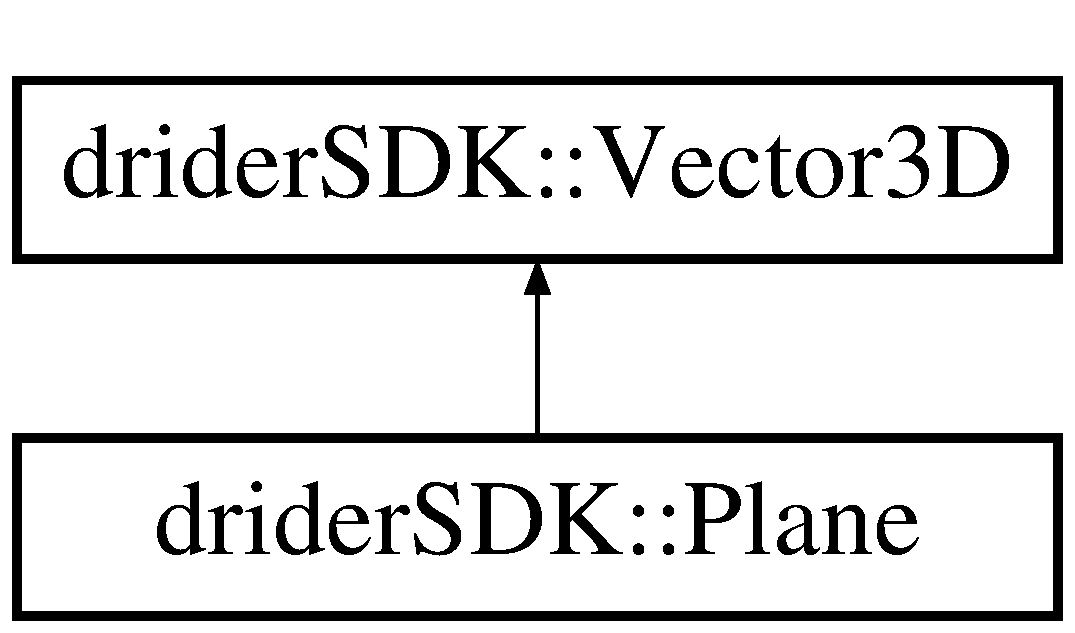
\includegraphics[height=2.000000cm]{classdrider_s_d_k_1_1_plane}
\end{center}
\end{figure}
\subsection*{Public Member Functions}
\begin{DoxyCompactItemize}
\item 
\hyperlink{classdrider_s_d_k_1_1_plane_a57f51d0d638c01f39ccf0ae6ff8fa2c0}{Plane} ()
\item 
\hyperlink{classdrider_s_d_k_1_1_plane_adef490d98a9ef2feda51c5b9e499aa50}{Plane} (const \hyperlink{classdrider_s_d_k_1_1_vector3_d}{Vector3D} \&\+\_\+normal, float \+\_\+d)
\item 
\hyperlink{classdrider_s_d_k_1_1_plane_a0560ff07d9e3b04b983a007f18470e23}{Plane} (const \hyperlink{classdrider_s_d_k_1_1_vector3_d}{Vector3D} \&\+\_\+normal, const \hyperlink{classdrider_s_d_k_1_1_vector3_d}{Vector3D} \&point)
\item 
\hyperlink{classdrider_s_d_k_1_1_plane_a4348d4b3f619cda528aa2512d6854538}{Plane} (const \hyperlink{classdrider_s_d_k_1_1_vector3_d}{Vector3D} \&point0, const \hyperlink{classdrider_s_d_k_1_1_vector3_d}{Vector3D} \&point1, const \hyperlink{classdrider_s_d_k_1_1_vector3_d}{Vector3D} \&point2)
\item 
\hyperlink{classdrider_s_d_k_1_1_plane_a8252aebcd126e8fe5b904513db658575}{Plane} (const \hyperlink{classdrider_s_d_k_1_1_plane}{Plane} \&)
\item 
\mbox{\Hypertarget{classdrider_s_d_k_1_1_plane_abf5cc0a71fae706c0d36d86d366963a0}\label{classdrider_s_d_k_1_1_plane_abf5cc0a71fae706c0d36d86d366963a0}} 
float {\bfseries distance\+To\+Point} (const \hyperlink{classdrider_s_d_k_1_1_vector3_d}{Vector3D} \&point)
\item 
float \hyperlink{classdrider_s_d_k_1_1_plane_a289ac3afd02981e3a1921846d9b14589}{signed\+Distance\+To\+Point} (const \hyperlink{classdrider_s_d_k_1_1_vector3_d}{Vector3D} \&point)
\item 
bool \hyperlink{classdrider_s_d_k_1_1_plane_a1dbd209dd564674cc1a4065fd089e3b2}{intersects} (const \hyperlink{classdrider_s_d_k_1_1_vector3_d}{Vector3D} \&point)
\item 
\mbox{\Hypertarget{classdrider_s_d_k_1_1_plane_a04f70d65529a37a11ea78e9dc18354ca}\label{classdrider_s_d_k_1_1_plane_a04f70d65529a37a11ea78e9dc18354ca}} 
bool {\bfseries intersects} (const \hyperlink{classdrider_s_d_k_1_1_plane}{Plane} \&other)
\item 
\mbox{\Hypertarget{classdrider_s_d_k_1_1_plane_aa24c91225bc02094376ade5569af7d57}\label{classdrider_s_d_k_1_1_plane_aa24c91225bc02094376ade5569af7d57}} 
bool {\bfseries intersects} (const \hyperlink{classdrider_s_d_k_1_1_sphere}{Sphere} \&sphere)
\item 
\mbox{\Hypertarget{classdrider_s_d_k_1_1_plane_a5d83ba5026cdff701430118eec2abe60}\label{classdrider_s_d_k_1_1_plane_a5d83ba5026cdff701430118eec2abe60}} 
bool {\bfseries intersects} (const \hyperlink{classdrider_s_d_k_1_1_a_a_b_b}{A\+A\+BB} \&aabb)
\item 
\mbox{\Hypertarget{classdrider_s_d_k_1_1_plane_a926d71fd601ac1407f18134327e18b61}\label{classdrider_s_d_k_1_1_plane_a926d71fd601ac1407f18134327e18b61}} 
bool {\bfseries intersects} (const \hyperlink{classdrider_s_d_k_1_1_capsule}{Capsule} \&capsule)
\item 
\mbox{\Hypertarget{classdrider_s_d_k_1_1_plane_aed121f4da95cb30477c49b59ff5e7ec4}\label{classdrider_s_d_k_1_1_plane_aed121f4da95cb30477c49b59ff5e7ec4}} 
bool {\bfseries intersects} (const \hyperlink{classdrider_s_d_k_1_1_frustrum}{Frustrum} \&frustrum)
\item 
void \hyperlink{classdrider_s_d_k_1_1_plane_ac8540b5c993e35b41baac2147fcbbc00}{normalize} ()
\item 
\mbox{\Hypertarget{classdrider_s_d_k_1_1_plane_a17bc82b2e68e62c492b6698c84a90039}\label{classdrider_s_d_k_1_1_plane_a17bc82b2e68e62c492b6698c84a90039}} 
\hyperlink{classdrider_s_d_k_1_1_plane}{Plane} \& {\bfseries operator=} (const \hyperlink{classdrider_s_d_k_1_1_plane}{Plane} \&other)
\item 
\mbox{\Hypertarget{classdrider_s_d_k_1_1_plane_afe19f5d245e70e16181cfab7172a2301}\label{classdrider_s_d_k_1_1_plane_afe19f5d245e70e16181cfab7172a2301}} 
bool {\bfseries operator==} (const \hyperlink{classdrider_s_d_k_1_1_plane}{Plane} \&rhs)
\item 
\mbox{\Hypertarget{classdrider_s_d_k_1_1_plane_a8e8e7ac10a3a8445bef69e7a97aa9bc8}\label{classdrider_s_d_k_1_1_plane_a8e8e7ac10a3a8445bef69e7a97aa9bc8}} 
bool {\bfseries operator!=} (const \hyperlink{classdrider_s_d_k_1_1_plane}{Plane} \&rhs)
\end{DoxyCompactItemize}
\subsection*{Public Attributes}
\begin{DoxyCompactItemize}
\item 
\mbox{\Hypertarget{classdrider_s_d_k_1_1_plane_a1c1e1e699f4f15d5930f09115de0de11}\label{classdrider_s_d_k_1_1_plane_a1c1e1e699f4f15d5930f09115de0de11}} 
float {\bfseries d}
\end{DoxyCompactItemize}


\subsection{Constructor \& Destructor Documentation}
\mbox{\Hypertarget{classdrider_s_d_k_1_1_plane_a57f51d0d638c01f39ccf0ae6ff8fa2c0}\label{classdrider_s_d_k_1_1_plane_a57f51d0d638c01f39ccf0ae6ff8fa2c0}} 
\index{drider\+S\+D\+K\+::\+Plane@{drider\+S\+D\+K\+::\+Plane}!Plane@{Plane}}
\index{Plane@{Plane}!drider\+S\+D\+K\+::\+Plane@{drider\+S\+D\+K\+::\+Plane}}
\subsubsection{\texorpdfstring{Plane()}{Plane()}\hspace{0.1cm}{\footnotesize\ttfamily [1/5]}}
{\footnotesize\ttfamily drider\+S\+D\+K\+::\+Plane\+::\+Plane (\begin{DoxyParamCaption}{ }\end{DoxyParamCaption})}

Default constructor. \mbox{\Hypertarget{classdrider_s_d_k_1_1_plane_adef490d98a9ef2feda51c5b9e499aa50}\label{classdrider_s_d_k_1_1_plane_adef490d98a9ef2feda51c5b9e499aa50}} 
\index{drider\+S\+D\+K\+::\+Plane@{drider\+S\+D\+K\+::\+Plane}!Plane@{Plane}}
\index{Plane@{Plane}!drider\+S\+D\+K\+::\+Plane@{drider\+S\+D\+K\+::\+Plane}}
\subsubsection{\texorpdfstring{Plane()}{Plane()}\hspace{0.1cm}{\footnotesize\ttfamily [2/5]}}
{\footnotesize\ttfamily drider\+S\+D\+K\+::\+Plane\+::\+Plane (\begin{DoxyParamCaption}\item[{const \hyperlink{classdrider_s_d_k_1_1_vector3_d}{Vector3D} \&}]{\+\_\+normal,  }\item[{float}]{\+\_\+d }\end{DoxyParamCaption})}

Constructor which takes a normal and a gap . \mbox{\Hypertarget{classdrider_s_d_k_1_1_plane_a0560ff07d9e3b04b983a007f18470e23}\label{classdrider_s_d_k_1_1_plane_a0560ff07d9e3b04b983a007f18470e23}} 
\index{drider\+S\+D\+K\+::\+Plane@{drider\+S\+D\+K\+::\+Plane}!Plane@{Plane}}
\index{Plane@{Plane}!drider\+S\+D\+K\+::\+Plane@{drider\+S\+D\+K\+::\+Plane}}
\subsubsection{\texorpdfstring{Plane()}{Plane()}\hspace{0.1cm}{\footnotesize\ttfamily [3/5]}}
{\footnotesize\ttfamily drider\+S\+D\+K\+::\+Plane\+::\+Plane (\begin{DoxyParamCaption}\item[{const \hyperlink{classdrider_s_d_k_1_1_vector3_d}{Vector3D} \&}]{\+\_\+normal,  }\item[{const \hyperlink{classdrider_s_d_k_1_1_vector3_d}{Vector3D} \&}]{point }\end{DoxyParamCaption})}

Constructor using a normal and a point to calculate the gap. \mbox{\Hypertarget{classdrider_s_d_k_1_1_plane_a4348d4b3f619cda528aa2512d6854538}\label{classdrider_s_d_k_1_1_plane_a4348d4b3f619cda528aa2512d6854538}} 
\index{drider\+S\+D\+K\+::\+Plane@{drider\+S\+D\+K\+::\+Plane}!Plane@{Plane}}
\index{Plane@{Plane}!drider\+S\+D\+K\+::\+Plane@{drider\+S\+D\+K\+::\+Plane}}
\subsubsection{\texorpdfstring{Plane()}{Plane()}\hspace{0.1cm}{\footnotesize\ttfamily [4/5]}}
{\footnotesize\ttfamily drider\+S\+D\+K\+::\+Plane\+::\+Plane (\begin{DoxyParamCaption}\item[{const \hyperlink{classdrider_s_d_k_1_1_vector3_d}{Vector3D} \&}]{point0,  }\item[{const \hyperlink{classdrider_s_d_k_1_1_vector3_d}{Vector3D} \&}]{point1,  }\item[{const \hyperlink{classdrider_s_d_k_1_1_vector3_d}{Vector3D} \&}]{point2 }\end{DoxyParamCaption})}

Constructor using 3 points in the plane which are used to calculate the normal of the plane and the gap. \mbox{\Hypertarget{classdrider_s_d_k_1_1_plane_a8252aebcd126e8fe5b904513db658575}\label{classdrider_s_d_k_1_1_plane_a8252aebcd126e8fe5b904513db658575}} 
\index{drider\+S\+D\+K\+::\+Plane@{drider\+S\+D\+K\+::\+Plane}!Plane@{Plane}}
\index{Plane@{Plane}!drider\+S\+D\+K\+::\+Plane@{drider\+S\+D\+K\+::\+Plane}}
\subsubsection{\texorpdfstring{Plane()}{Plane()}\hspace{0.1cm}{\footnotesize\ttfamily [5/5]}}
{\footnotesize\ttfamily drider\+S\+D\+K\+::\+Plane\+::\+Plane (\begin{DoxyParamCaption}\item[{const \hyperlink{classdrider_s_d_k_1_1_plane}{Plane} \&}]{other }\end{DoxyParamCaption})}

Copy constructor 

\subsection{Member Function Documentation}
\mbox{\Hypertarget{classdrider_s_d_k_1_1_plane_a1dbd209dd564674cc1a4065fd089e3b2}\label{classdrider_s_d_k_1_1_plane_a1dbd209dd564674cc1a4065fd089e3b2}} 
\index{drider\+S\+D\+K\+::\+Plane@{drider\+S\+D\+K\+::\+Plane}!intersects@{intersects}}
\index{intersects@{intersects}!drider\+S\+D\+K\+::\+Plane@{drider\+S\+D\+K\+::\+Plane}}
\subsubsection{\texorpdfstring{intersects()}{intersects()}}
{\footnotesize\ttfamily bool drider\+S\+D\+K\+::\+Plane\+::intersects (\begin{DoxyParamCaption}\item[{const \hyperlink{classdrider_s_d_k_1_1_vector3_d}{Vector3D} \&}]{point }\end{DoxyParamCaption})}

Computes the intersection with a point

\begin{DoxyReturn}{Returns}
True if the point is in the plane, false otherwise 
\end{DoxyReturn}
\mbox{\Hypertarget{classdrider_s_d_k_1_1_plane_ac8540b5c993e35b41baac2147fcbbc00}\label{classdrider_s_d_k_1_1_plane_ac8540b5c993e35b41baac2147fcbbc00}} 
\index{drider\+S\+D\+K\+::\+Plane@{drider\+S\+D\+K\+::\+Plane}!normalize@{normalize}}
\index{normalize@{normalize}!drider\+S\+D\+K\+::\+Plane@{drider\+S\+D\+K\+::\+Plane}}
\subsubsection{\texorpdfstring{normalize()}{normalize()}}
{\footnotesize\ttfamily void drider\+S\+D\+K\+::\+Plane\+::normalize (\begin{DoxyParamCaption}{ }\end{DoxyParamCaption})}

Gets the plane normalized

\begin{DoxyReturn}{Returns}
The plane normalized. 
\end{DoxyReturn}
\mbox{\Hypertarget{classdrider_s_d_k_1_1_plane_a289ac3afd02981e3a1921846d9b14589}\label{classdrider_s_d_k_1_1_plane_a289ac3afd02981e3a1921846d9b14589}} 
\index{drider\+S\+D\+K\+::\+Plane@{drider\+S\+D\+K\+::\+Plane}!signed\+Distance\+To\+Point@{signed\+Distance\+To\+Point}}
\index{signed\+Distance\+To\+Point@{signed\+Distance\+To\+Point}!drider\+S\+D\+K\+::\+Plane@{drider\+S\+D\+K\+::\+Plane}}
\subsubsection{\texorpdfstring{signed\+Distance\+To\+Point()}{signedDistanceToPoint()}}
{\footnotesize\ttfamily float drider\+S\+D\+K\+::\+Plane\+::signed\+Distance\+To\+Point (\begin{DoxyParamCaption}\item[{const \hyperlink{classdrider_s_d_k_1_1_vector3_d}{Vector3D} \&}]{point }\end{DoxyParamCaption})}

Computes the signed distance to a point.


\begin{DoxyParams}{Parameters}
{\em point} & The point used to calculate the distance.\\
\hline
\end{DoxyParams}
\begin{DoxyReturn}{Returns}
The signed distance to the point, this is useful to know if a point is behind or in front of the plane. 
\end{DoxyReturn}


The documentation for this class was generated from the following files\+:\begin{DoxyCompactItemize}
\item 
C\+:/\+Users/\+Francisco/source/repos/\+Drider-\/\+Engine/\+Math/\+Include/dr\+\_\+plane.\+h\item 
C\+:/\+Users/\+Francisco/source/repos/\+Drider-\/\+Engine/\+Math/\+Source/dr\+\_\+plane.\+cpp\end{DoxyCompactItemize}

\hypertarget{classdrider_s_d_k_1_1_pool}{}\section{drider\+S\+DK\+:\+:Pool$<$ T, pool\+Size $>$ Class Template Reference}
\label{classdrider_s_d_k_1_1_pool}\index{drider\+S\+D\+K\+::\+Pool$<$ T, pool\+Size $>$@{drider\+S\+D\+K\+::\+Pool$<$ T, pool\+Size $>$}}
\subsection*{Public Member Functions}
\begin{DoxyCompactItemize}
\item 
\mbox{\Hypertarget{classdrider_s_d_k_1_1_pool_af13ebb482203072260ddea104b4f433e}\label{classdrider_s_d_k_1_1_pool_af13ebb482203072260ddea104b4f433e}} 
T $\ast$ {\bfseries aquire} ()
\end{DoxyCompactItemize}
\subsection*{Private Attributes}
\begin{DoxyCompactItemize}
\item 
\mbox{\Hypertarget{classdrider_s_d_k_1_1_pool_a9634dac3a39c5fcd26f8a54e26b04082}\label{classdrider_s_d_k_1_1_pool_a9634dac3a39c5fcd26f8a54e26b04082}} 
std\+::vector$<$ std\+::unique\+\_\+ptr$<$ T $>$ $>$ {\bfseries m\+\_\+pool}
\item 
\mbox{\Hypertarget{classdrider_s_d_k_1_1_pool_a12c1fa9f40c34670736e4ae535afbf83}\label{classdrider_s_d_k_1_1_pool_a12c1fa9f40c34670736e4ae535afbf83}} 
U\+Int32 {\bfseries m\+\_\+next\+Object\+Index}
\end{DoxyCompactItemize}


The documentation for this class was generated from the following file\+:\begin{DoxyCompactItemize}
\item 
C\+:/\+Users/\+Francisco/source/repos/\+Drider-\/\+Engine/\+Utils/\+Include/dr\+\_\+pool.\+h\end{DoxyCompactItemize}

\hypertarget{classdrider_s_d_k_1_1_quaternion}{}\section{drider\+S\+DK\+:\+:Quaternion Class Reference}
\label{classdrider_s_d_k_1_1_quaternion}\index{drider\+S\+D\+K\+::\+Quaternion@{drider\+S\+D\+K\+::\+Quaternion}}
\subsection*{Public Member Functions}
\begin{DoxyCompactItemize}
\item 
\hyperlink{classdrider_s_d_k_1_1_quaternion_ae022b897e4f962cf3a7f5a155ad01234}{Quaternion} ()
\item 
\hyperlink{classdrider_s_d_k_1_1_quaternion_a644b649dee7047182a31d10d087062ca}{Quaternion} (\hyperlink{classdrider_s_d_k_1_1_quaternion}{Quaternion} \&\&Q)=default
\item 
\hyperlink{classdrider_s_d_k_1_1_quaternion_ad90008123c45fcdf2a92ba25028101dd}{Quaternion} (const \hyperlink{classdrider_s_d_k_1_1_quaternion}{Quaternion} \&Q)
\item 
\hyperlink{classdrider_s_d_k_1_1_quaternion_a9b9b7fe9fbfbf24c911dbd6ca7ff2df2}{Quaternion} (float x, float y, float z, float w)
\item 
\hyperlink{classdrider_s_d_k_1_1_quaternion_a5ab8ae4293dfd405fc11c4a0114209b4}{$\sim$\+Quaternion} ()
\item 
float \hyperlink{classdrider_s_d_k_1_1_quaternion_af549c85e1b2e1a67668a193cf66da927}{measure} ()
\item 
\hyperlink{classdrider_s_d_k_1_1_quaternion}{Quaternion} \hyperlink{classdrider_s_d_k_1_1_quaternion_aa2f2f19f27b36910669f84acb1e88f8f}{conjugate} ()
\item 
\hyperlink{classdrider_s_d_k_1_1_quaternion}{Quaternion} \hyperlink{classdrider_s_d_k_1_1_quaternion_afd671db56c3cd55b0d543e96b8e690ef}{normalize} ()
\item 
\hyperlink{classdrider_s_d_k_1_1_quaternion}{Quaternion} \hyperlink{classdrider_s_d_k_1_1_quaternion_a892aa4383f2070ef76b549705b8905cb}{rotation} (float theta, const \hyperlink{classdrider_s_d_k_1_1_quaternion}{Quaternion} \&A)
\item 
void \hyperlink{classdrider_s_d_k_1_1_quaternion_a2fd752f214ccf84e6bdad3c7a21f0e7f}{matrix\+From\+Quaternion} (\hyperlink{classdrider_s_d_k_1_1_matrix4x4}{Matrix4x4} \&Matrix)
\item 
\mbox{\Hypertarget{classdrider_s_d_k_1_1_quaternion_ae6ab63972d92e470e6c86948298f8e77}\label{classdrider_s_d_k_1_1_quaternion_ae6ab63972d92e470e6c86948298f8e77}} 
\hyperlink{classdrider_s_d_k_1_1_quaternion}{Quaternion} {\bfseries operator+} (const \hyperlink{classdrider_s_d_k_1_1_quaternion}{Quaternion} \&Q) const
\item 
\mbox{\Hypertarget{classdrider_s_d_k_1_1_quaternion_ac8a2a66381f88fa96c6245ef8799f862}\label{classdrider_s_d_k_1_1_quaternion_ac8a2a66381f88fa96c6245ef8799f862}} 
\hyperlink{classdrider_s_d_k_1_1_quaternion}{Quaternion} \& {\bfseries operator+=} (const \hyperlink{classdrider_s_d_k_1_1_quaternion}{Quaternion} \&Q)
\item 
\mbox{\Hypertarget{classdrider_s_d_k_1_1_quaternion_a978177401980f55d74ece0b1601c71cc}\label{classdrider_s_d_k_1_1_quaternion_a978177401980f55d74ece0b1601c71cc}} 
\hyperlink{classdrider_s_d_k_1_1_quaternion}{Quaternion} {\bfseries operator-\/} (const \hyperlink{classdrider_s_d_k_1_1_quaternion}{Quaternion} \&Q) const
\item 
\mbox{\Hypertarget{classdrider_s_d_k_1_1_quaternion_ac0e42f6f2256fc1999fc7e74a19263f0}\label{classdrider_s_d_k_1_1_quaternion_ac0e42f6f2256fc1999fc7e74a19263f0}} 
\hyperlink{classdrider_s_d_k_1_1_quaternion}{Quaternion} \& {\bfseries operator-\/=} (const \hyperlink{classdrider_s_d_k_1_1_quaternion}{Quaternion} \&Q)
\item 
\mbox{\Hypertarget{classdrider_s_d_k_1_1_quaternion_ad7ea7df44436b84bf9d7935b7bbd7e45}\label{classdrider_s_d_k_1_1_quaternion_ad7ea7df44436b84bf9d7935b7bbd7e45}} 
\hyperlink{classdrider_s_d_k_1_1_quaternion}{Quaternion} {\bfseries operator$\ast$} (const \hyperlink{classdrider_s_d_k_1_1_quaternion}{Quaternion} \&Q) const
\item 
\mbox{\Hypertarget{classdrider_s_d_k_1_1_quaternion_a16955a9b7daad26e5a04f41a4d495508}\label{classdrider_s_d_k_1_1_quaternion_a16955a9b7daad26e5a04f41a4d495508}} 
\hyperlink{classdrider_s_d_k_1_1_quaternion}{Quaternion} {\bfseries operator$\ast$} (float s) const
\item 
\mbox{\Hypertarget{classdrider_s_d_k_1_1_quaternion_ad45b068286bcbfa65130d664d67c3576}\label{classdrider_s_d_k_1_1_quaternion_ad45b068286bcbfa65130d664d67c3576}} 
\hyperlink{classdrider_s_d_k_1_1_quaternion}{Quaternion} \& {\bfseries operator$\ast$=} (const \hyperlink{classdrider_s_d_k_1_1_quaternion}{Quaternion} \&Q)
\item 
\mbox{\Hypertarget{classdrider_s_d_k_1_1_quaternion_aadb86445d5c10d9e5d60c15a537d1ed6}\label{classdrider_s_d_k_1_1_quaternion_aadb86445d5c10d9e5d60c15a537d1ed6}} 
\hyperlink{classdrider_s_d_k_1_1_quaternion}{Quaternion} \& {\bfseries operator$\ast$=} (float s)
\item 
\mbox{\Hypertarget{classdrider_s_d_k_1_1_quaternion_a2bcae404a0cb030490b618f19140adf5}\label{classdrider_s_d_k_1_1_quaternion_a2bcae404a0cb030490b618f19140adf5}} 
\hyperlink{classdrider_s_d_k_1_1_quaternion}{Quaternion} {\bfseries operator/} (const \hyperlink{classdrider_s_d_k_1_1_quaternion}{Quaternion} \&Q) const
\item 
\mbox{\Hypertarget{classdrider_s_d_k_1_1_quaternion_a67e8465383eed2f429ddce83a07a8d7d}\label{classdrider_s_d_k_1_1_quaternion_a67e8465383eed2f429ddce83a07a8d7d}} 
\hyperlink{classdrider_s_d_k_1_1_quaternion}{Quaternion} \& {\bfseries operator/=} (const \hyperlink{classdrider_s_d_k_1_1_quaternion}{Quaternion} \&Q)
\end{DoxyCompactItemize}
\subsection*{Public Attributes}
\begin{DoxyCompactItemize}
\item 
\mbox{\Hypertarget{classdrider_s_d_k_1_1_quaternion_a5ef3bca21e0b6e3e475108eb93ab1e40}\label{classdrider_s_d_k_1_1_quaternion_a5ef3bca21e0b6e3e475108eb93ab1e40}} 
\begin{tabbing}
xx\=xx\=xx\=xx\=xx\=xx\=xx\=xx\=xx\=\kill
union \{\\
\mbox{\Hypertarget{uniondrider_s_d_k_1_1_quaternion_1_1_0D8_a1e032a7dbbf531b64519917ee2968ec7}\label{uniondrider_s_d_k_1_1_quaternion_1_1_0D8_a1e032a7dbbf531b64519917ee2968ec7}} 
\>struct \{\\
\>\>float {\bfseries x}\\
\>\>float {\bfseries y}\\
\>\>float {\bfseries z}\\
\>\>float {\bfseries w}\\
\>\} \\
\>float {\bfseries data} \mbox{[}4\mbox{]}\\
\}; \\

\end{tabbing}\end{DoxyCompactItemize}


\subsection{Constructor \& Destructor Documentation}
\mbox{\Hypertarget{classdrider_s_d_k_1_1_quaternion_ae022b897e4f962cf3a7f5a155ad01234}\label{classdrider_s_d_k_1_1_quaternion_ae022b897e4f962cf3a7f5a155ad01234}} 
\index{drider\+S\+D\+K\+::\+Quaternion@{drider\+S\+D\+K\+::\+Quaternion}!Quaternion@{Quaternion}}
\index{Quaternion@{Quaternion}!drider\+S\+D\+K\+::\+Quaternion@{drider\+S\+D\+K\+::\+Quaternion}}
\subsubsection{\texorpdfstring{Quaternion()}{Quaternion()}\hspace{0.1cm}{\footnotesize\ttfamily [1/4]}}
{\footnotesize\ttfamily drider\+S\+D\+K\+::\+Quaternion\+::\+Quaternion (\begin{DoxyParamCaption}{ }\end{DoxyParamCaption})}

Default constructor. \mbox{\Hypertarget{classdrider_s_d_k_1_1_quaternion_a644b649dee7047182a31d10d087062ca}\label{classdrider_s_d_k_1_1_quaternion_a644b649dee7047182a31d10d087062ca}} 
\index{drider\+S\+D\+K\+::\+Quaternion@{drider\+S\+D\+K\+::\+Quaternion}!Quaternion@{Quaternion}}
\index{Quaternion@{Quaternion}!drider\+S\+D\+K\+::\+Quaternion@{drider\+S\+D\+K\+::\+Quaternion}}
\subsubsection{\texorpdfstring{Quaternion()}{Quaternion()}\hspace{0.1cm}{\footnotesize\ttfamily [2/4]}}
{\footnotesize\ttfamily drider\+S\+D\+K\+::\+Quaternion\+::\+Quaternion (\begin{DoxyParamCaption}\item[{\hyperlink{classdrider_s_d_k_1_1_quaternion}{Quaternion} \&\&}]{Q }\end{DoxyParamCaption})\hspace{0.3cm}{\ttfamily [default]}}

Move constructor. \mbox{\Hypertarget{classdrider_s_d_k_1_1_quaternion_ad90008123c45fcdf2a92ba25028101dd}\label{classdrider_s_d_k_1_1_quaternion_ad90008123c45fcdf2a92ba25028101dd}} 
\index{drider\+S\+D\+K\+::\+Quaternion@{drider\+S\+D\+K\+::\+Quaternion}!Quaternion@{Quaternion}}
\index{Quaternion@{Quaternion}!drider\+S\+D\+K\+::\+Quaternion@{drider\+S\+D\+K\+::\+Quaternion}}
\subsubsection{\texorpdfstring{Quaternion()}{Quaternion()}\hspace{0.1cm}{\footnotesize\ttfamily [3/4]}}
{\footnotesize\ttfamily drider\+S\+D\+K\+::\+Quaternion\+::\+Quaternion (\begin{DoxyParamCaption}\item[{const \hyperlink{classdrider_s_d_k_1_1_quaternion}{Quaternion} \&}]{Q }\end{DoxyParamCaption})}

Copy constructor. \mbox{\Hypertarget{classdrider_s_d_k_1_1_quaternion_a9b9b7fe9fbfbf24c911dbd6ca7ff2df2}\label{classdrider_s_d_k_1_1_quaternion_a9b9b7fe9fbfbf24c911dbd6ca7ff2df2}} 
\index{drider\+S\+D\+K\+::\+Quaternion@{drider\+S\+D\+K\+::\+Quaternion}!Quaternion@{Quaternion}}
\index{Quaternion@{Quaternion}!drider\+S\+D\+K\+::\+Quaternion@{drider\+S\+D\+K\+::\+Quaternion}}
\subsubsection{\texorpdfstring{Quaternion()}{Quaternion()}\hspace{0.1cm}{\footnotesize\ttfamily [4/4]}}
{\footnotesize\ttfamily drider\+S\+D\+K\+::\+Quaternion\+::\+Quaternion (\begin{DoxyParamCaption}\item[{float}]{x,  }\item[{float}]{y,  }\item[{float}]{z,  }\item[{float}]{w }\end{DoxyParamCaption})}

Initialize the constructor with the given values.


\begin{DoxyParams}{Parameters}
{\em x} & The x value of the quaternion.\\
\hline
{\em y} & The y value of the quaternion.\\
\hline
{\em z} & The z value of the quaternion.\\
\hline
{\em w} & The w value of the quaternion. \\
\hline
\end{DoxyParams}
\mbox{\Hypertarget{classdrider_s_d_k_1_1_quaternion_a5ab8ae4293dfd405fc11c4a0114209b4}\label{classdrider_s_d_k_1_1_quaternion_a5ab8ae4293dfd405fc11c4a0114209b4}} 
\index{drider\+S\+D\+K\+::\+Quaternion@{drider\+S\+D\+K\+::\+Quaternion}!````~Quaternion@{$\sim$\+Quaternion}}
\index{````~Quaternion@{$\sim$\+Quaternion}!drider\+S\+D\+K\+::\+Quaternion@{drider\+S\+D\+K\+::\+Quaternion}}
\subsubsection{\texorpdfstring{$\sim$\+Quaternion()}{~Quaternion()}}
{\footnotesize\ttfamily drider\+S\+D\+K\+::\+Quaternion\+::$\sim$\+Quaternion (\begin{DoxyParamCaption}{ }\end{DoxyParamCaption})}

Default destructor. 

\subsection{Member Function Documentation}
\mbox{\Hypertarget{classdrider_s_d_k_1_1_quaternion_aa2f2f19f27b36910669f84acb1e88f8f}\label{classdrider_s_d_k_1_1_quaternion_aa2f2f19f27b36910669f84acb1e88f8f}} 
\index{drider\+S\+D\+K\+::\+Quaternion@{drider\+S\+D\+K\+::\+Quaternion}!conjugate@{conjugate}}
\index{conjugate@{conjugate}!drider\+S\+D\+K\+::\+Quaternion@{drider\+S\+D\+K\+::\+Quaternion}}
\subsubsection{\texorpdfstring{conjugate()}{conjugate()}}
{\footnotesize\ttfamily \hyperlink{classdrider_s_d_k_1_1_quaternion}{Quaternion} drider\+S\+D\+K\+::\+Quaternion\+::conjugate (\begin{DoxyParamCaption}{ }\end{DoxyParamCaption})}

Computes the conjugate of the quaternion.

\begin{DoxyReturn}{Returns}
The conjugate quaternion. 
\end{DoxyReturn}
\mbox{\Hypertarget{classdrider_s_d_k_1_1_quaternion_a2fd752f214ccf84e6bdad3c7a21f0e7f}\label{classdrider_s_d_k_1_1_quaternion_a2fd752f214ccf84e6bdad3c7a21f0e7f}} 
\index{drider\+S\+D\+K\+::\+Quaternion@{drider\+S\+D\+K\+::\+Quaternion}!matrix\+From\+Quaternion@{matrix\+From\+Quaternion}}
\index{matrix\+From\+Quaternion@{matrix\+From\+Quaternion}!drider\+S\+D\+K\+::\+Quaternion@{drider\+S\+D\+K\+::\+Quaternion}}
\subsubsection{\texorpdfstring{matrix\+From\+Quaternion()}{matrixFromQuaternion()}}
{\footnotesize\ttfamily void drider\+S\+D\+K\+::\+Quaternion\+::matrix\+From\+Quaternion (\begin{DoxyParamCaption}\item[{\hyperlink{classdrider_s_d_k_1_1_matrix4x4}{Matrix4x4} \&}]{Matrix }\end{DoxyParamCaption})}

Creates a matrix from the quaternion.


\begin{DoxyParams}{Parameters}
{\em Matrix} & \hyperlink{classdrider_s_d_k_1_1_matrix4x4}{Matrix4x4} to be filled. \\
\hline
\end{DoxyParams}
\mbox{\Hypertarget{classdrider_s_d_k_1_1_quaternion_af549c85e1b2e1a67668a193cf66da927}\label{classdrider_s_d_k_1_1_quaternion_af549c85e1b2e1a67668a193cf66da927}} 
\index{drider\+S\+D\+K\+::\+Quaternion@{drider\+S\+D\+K\+::\+Quaternion}!measure@{measure}}
\index{measure@{measure}!drider\+S\+D\+K\+::\+Quaternion@{drider\+S\+D\+K\+::\+Quaternion}}
\subsubsection{\texorpdfstring{measure()}{measure()}}
{\footnotesize\ttfamily float drider\+S\+D\+K\+::\+Quaternion\+::measure (\begin{DoxyParamCaption}{ }\end{DoxyParamCaption})}

Computes the measure of the quaternion.

\begin{DoxyReturn}{Returns}
\hyperlink{classdrider_s_d_k_1_1_quaternion}{Quaternion}\textquotesingle{}s lenght. 
\end{DoxyReturn}
\mbox{\Hypertarget{classdrider_s_d_k_1_1_quaternion_afd671db56c3cd55b0d543e96b8e690ef}\label{classdrider_s_d_k_1_1_quaternion_afd671db56c3cd55b0d543e96b8e690ef}} 
\index{drider\+S\+D\+K\+::\+Quaternion@{drider\+S\+D\+K\+::\+Quaternion}!normalize@{normalize}}
\index{normalize@{normalize}!drider\+S\+D\+K\+::\+Quaternion@{drider\+S\+D\+K\+::\+Quaternion}}
\subsubsection{\texorpdfstring{normalize()}{normalize()}}
{\footnotesize\ttfamily \hyperlink{classdrider_s_d_k_1_1_quaternion}{Quaternion} drider\+S\+D\+K\+::\+Quaternion\+::normalize (\begin{DoxyParamCaption}{ }\end{DoxyParamCaption})}

Computes the normalized quaternion.

\begin{DoxyReturn}{Returns}
This normalized quaternion. 
\end{DoxyReturn}
\mbox{\Hypertarget{classdrider_s_d_k_1_1_quaternion_a892aa4383f2070ef76b549705b8905cb}\label{classdrider_s_d_k_1_1_quaternion_a892aa4383f2070ef76b549705b8905cb}} 
\index{drider\+S\+D\+K\+::\+Quaternion@{drider\+S\+D\+K\+::\+Quaternion}!rotation@{rotation}}
\index{rotation@{rotation}!drider\+S\+D\+K\+::\+Quaternion@{drider\+S\+D\+K\+::\+Quaternion}}
\subsubsection{\texorpdfstring{rotation()}{rotation()}}
{\footnotesize\ttfamily \hyperlink{classdrider_s_d_k_1_1_quaternion}{Quaternion} drider\+S\+D\+K\+::\+Quaternion\+::rotation (\begin{DoxyParamCaption}\item[{float}]{theta,  }\item[{const \hyperlink{classdrider_s_d_k_1_1_quaternion}{Quaternion} \&}]{A }\end{DoxyParamCaption})}

Rotates the quaternion given theta and another quaternion.


\begin{DoxyParams}{Parameters}
{\em theta} & Angle of rotation.\\
\hline
{\em A} & The other quaternion to generate an axis.\\
\hline
\end{DoxyParams}
\begin{DoxyReturn}{Returns}
A rotated quaternion. 
\end{DoxyReturn}


The documentation for this class was generated from the following files\+:\begin{DoxyCompactItemize}
\item 
C\+:/\+Users/\+Francisco/source/repos/\+Drider-\/\+Engine/\+Math/\+Include/dr\+\_\+quaternion.\+h\item 
C\+:/\+Users/\+Francisco/source/repos/\+Drider-\/\+Engine/\+Math/\+Source/dr\+\_\+quaternion.\+cpp\end{DoxyCompactItemize}

\hypertarget{classdrider_s_d_k_1_1_radian}{}\section{drider\+S\+DK\+:\+:Radian Class Reference}
\label{classdrider_s_d_k_1_1_radian}\index{drider\+S\+D\+K\+::\+Radian@{drider\+S\+D\+K\+::\+Radian}}
\subsection*{Public Member Functions}
\begin{DoxyCompactItemize}
\item 
\hyperlink{classdrider_s_d_k_1_1_radian_a3e670b9e0a28e363b8b20645e2962c66}{Radian} ()
\item 
\hyperlink{classdrider_s_d_k_1_1_radian_a3f93a33ebb6195d6732bff6262a4c91c}{Radian} (\hyperlink{classdrider_s_d_k_1_1_radian}{Radian} \&\&V)=default
\item 
\hyperlink{classdrider_s_d_k_1_1_radian_a8487633584761b8cabbe182cf26f5168}{Radian} (const \hyperlink{classdrider_s_d_k_1_1_radian}{Radian} \&V)
\item 
\hyperlink{classdrider_s_d_k_1_1_radian_a21d244cf4c918a5658b69dd1b4df2d6e}{Radian} (float value)
\item 
\hyperlink{classdrider_s_d_k_1_1_radian_a9b1711276eed04187623b4cb047c90ce}{$\sim$\+Radian} ()
\item 
float \hyperlink{classdrider_s_d_k_1_1_radian_a2b848dd9f60fbdb8e113620e9933f3d8}{to\+Degree} () const
\item 
\hyperlink{classdrider_s_d_k_1_1_radian}{Radian} \& \hyperlink{classdrider_s_d_k_1_1_radian_ac9d138249e554f129d2ffc0ddb39b881}{unwind} ()
\item 
\mbox{\Hypertarget{classdrider_s_d_k_1_1_radian_abcf6e621b7842bf900ef194a0506dcaf}\label{classdrider_s_d_k_1_1_radian_abcf6e621b7842bf900ef194a0506dcaf}} 
{\bfseries operator float} ()
\item 
\mbox{\Hypertarget{classdrider_s_d_k_1_1_radian_aca76d9162983d1a6cc372abdc0ae4c33}\label{classdrider_s_d_k_1_1_radian_aca76d9162983d1a6cc372abdc0ae4c33}} 
\hyperlink{classdrider_s_d_k_1_1_radian}{Radian} \& {\bfseries operator=} (float V)
\item 
\mbox{\Hypertarget{classdrider_s_d_k_1_1_radian_a13e910cd2706b9c5faf6498329267a2c}\label{classdrider_s_d_k_1_1_radian_a13e910cd2706b9c5faf6498329267a2c}} 
\hyperlink{classdrider_s_d_k_1_1_radian}{Radian} \& {\bfseries operator+=} (float V)
\item 
\mbox{\Hypertarget{classdrider_s_d_k_1_1_radian_a9746d00ab6b2d02d7ceee3dfe8336226}\label{classdrider_s_d_k_1_1_radian_a9746d00ab6b2d02d7ceee3dfe8336226}} 
\hyperlink{classdrider_s_d_k_1_1_radian}{Radian} \& {\bfseries operator-\/=} (float V)
\item 
\mbox{\Hypertarget{classdrider_s_d_k_1_1_radian_ac2693a74811ab733afdeaa12c492f264}\label{classdrider_s_d_k_1_1_radian_ac2693a74811ab733afdeaa12c492f264}} 
\hyperlink{classdrider_s_d_k_1_1_radian}{Radian} \& {\bfseries operator$\ast$=} (float V)
\item 
\mbox{\Hypertarget{classdrider_s_d_k_1_1_radian_a61a961f132fb81e6366291e9cd8ed7e1}\label{classdrider_s_d_k_1_1_radian_a61a961f132fb81e6366291e9cd8ed7e1}} 
\hyperlink{classdrider_s_d_k_1_1_radian}{Radian} \& {\bfseries operator/=} (float V)
\end{DoxyCompactItemize}
\subsection*{Private Attributes}
\begin{DoxyCompactItemize}
\item 
\mbox{\Hypertarget{classdrider_s_d_k_1_1_radian_a3a10447cdeefbfafd08a8e0187f42d91}\label{classdrider_s_d_k_1_1_radian_a3a10447cdeefbfafd08a8e0187f42d91}} 
float {\bfseries m\+\_\+value}
\end{DoxyCompactItemize}


\subsection{Constructor \& Destructor Documentation}
\mbox{\Hypertarget{classdrider_s_d_k_1_1_radian_a3e670b9e0a28e363b8b20645e2962c66}\label{classdrider_s_d_k_1_1_radian_a3e670b9e0a28e363b8b20645e2962c66}} 
\index{drider\+S\+D\+K\+::\+Radian@{drider\+S\+D\+K\+::\+Radian}!Radian@{Radian}}
\index{Radian@{Radian}!drider\+S\+D\+K\+::\+Radian@{drider\+S\+D\+K\+::\+Radian}}
\subsubsection{\texorpdfstring{Radian()}{Radian()}\hspace{0.1cm}{\footnotesize\ttfamily [1/4]}}
{\footnotesize\ttfamily drider\+S\+D\+K\+::\+Radian\+::\+Radian (\begin{DoxyParamCaption}{ }\end{DoxyParamCaption})}

Default constructor. \mbox{\Hypertarget{classdrider_s_d_k_1_1_radian_a3f93a33ebb6195d6732bff6262a4c91c}\label{classdrider_s_d_k_1_1_radian_a3f93a33ebb6195d6732bff6262a4c91c}} 
\index{drider\+S\+D\+K\+::\+Radian@{drider\+S\+D\+K\+::\+Radian}!Radian@{Radian}}
\index{Radian@{Radian}!drider\+S\+D\+K\+::\+Radian@{drider\+S\+D\+K\+::\+Radian}}
\subsubsection{\texorpdfstring{Radian()}{Radian()}\hspace{0.1cm}{\footnotesize\ttfamily [2/4]}}
{\footnotesize\ttfamily drider\+S\+D\+K\+::\+Radian\+::\+Radian (\begin{DoxyParamCaption}\item[{\hyperlink{classdrider_s_d_k_1_1_radian}{Radian} \&\&}]{V }\end{DoxyParamCaption})\hspace{0.3cm}{\ttfamily [default]}}

Move constructor. \mbox{\Hypertarget{classdrider_s_d_k_1_1_radian_a8487633584761b8cabbe182cf26f5168}\label{classdrider_s_d_k_1_1_radian_a8487633584761b8cabbe182cf26f5168}} 
\index{drider\+S\+D\+K\+::\+Radian@{drider\+S\+D\+K\+::\+Radian}!Radian@{Radian}}
\index{Radian@{Radian}!drider\+S\+D\+K\+::\+Radian@{drider\+S\+D\+K\+::\+Radian}}
\subsubsection{\texorpdfstring{Radian()}{Radian()}\hspace{0.1cm}{\footnotesize\ttfamily [3/4]}}
{\footnotesize\ttfamily drider\+S\+D\+K\+::\+Radian\+::\+Radian (\begin{DoxyParamCaption}\item[{const \hyperlink{classdrider_s_d_k_1_1_radian}{Radian} \&}]{V }\end{DoxyParamCaption})}

Copy constructor. \mbox{\Hypertarget{classdrider_s_d_k_1_1_radian_a21d244cf4c918a5658b69dd1b4df2d6e}\label{classdrider_s_d_k_1_1_radian_a21d244cf4c918a5658b69dd1b4df2d6e}} 
\index{drider\+S\+D\+K\+::\+Radian@{drider\+S\+D\+K\+::\+Radian}!Radian@{Radian}}
\index{Radian@{Radian}!drider\+S\+D\+K\+::\+Radian@{drider\+S\+D\+K\+::\+Radian}}
\subsubsection{\texorpdfstring{Radian()}{Radian()}\hspace{0.1cm}{\footnotesize\ttfamily [4/4]}}
{\footnotesize\ttfamily drider\+S\+D\+K\+::\+Radian\+::\+Radian (\begin{DoxyParamCaption}\item[{float}]{value }\end{DoxyParamCaption})\hspace{0.3cm}{\ttfamily [explicit]}}

Initialize class with value.


\begin{DoxyParams}{Parameters}
{\em value} & Initial value. \\
\hline
\end{DoxyParams}
\mbox{\Hypertarget{classdrider_s_d_k_1_1_radian_a9b1711276eed04187623b4cb047c90ce}\label{classdrider_s_d_k_1_1_radian_a9b1711276eed04187623b4cb047c90ce}} 
\index{drider\+S\+D\+K\+::\+Radian@{drider\+S\+D\+K\+::\+Radian}!````~Radian@{$\sim$\+Radian}}
\index{````~Radian@{$\sim$\+Radian}!drider\+S\+D\+K\+::\+Radian@{drider\+S\+D\+K\+::\+Radian}}
\subsubsection{\texorpdfstring{$\sim$\+Radian()}{~Radian()}}
{\footnotesize\ttfamily drider\+S\+D\+K\+::\+Radian\+::$\sim$\+Radian (\begin{DoxyParamCaption}{ }\end{DoxyParamCaption})}

Default destructor. 

\subsection{Member Function Documentation}
\mbox{\Hypertarget{classdrider_s_d_k_1_1_radian_a2b848dd9f60fbdb8e113620e9933f3d8}\label{classdrider_s_d_k_1_1_radian_a2b848dd9f60fbdb8e113620e9933f3d8}} 
\index{drider\+S\+D\+K\+::\+Radian@{drider\+S\+D\+K\+::\+Radian}!to\+Degree@{to\+Degree}}
\index{to\+Degree@{to\+Degree}!drider\+S\+D\+K\+::\+Radian@{drider\+S\+D\+K\+::\+Radian}}
\subsubsection{\texorpdfstring{to\+Degree()}{toDegree()}}
{\footnotesize\ttfamily float drider\+S\+D\+K\+::\+Radian\+::to\+Degree (\begin{DoxyParamCaption}{ }\end{DoxyParamCaption}) const}

Returns a \hyperlink{classdrider_s_d_k_1_1_degree}{Degree} class with a value equal to the actual radian in degrees.

\begin{DoxyReturn}{Returns}
Class degree. 
\end{DoxyReturn}
\mbox{\Hypertarget{classdrider_s_d_k_1_1_radian_ac9d138249e554f129d2ffc0ddb39b881}\label{classdrider_s_d_k_1_1_radian_ac9d138249e554f129d2ffc0ddb39b881}} 
\index{drider\+S\+D\+K\+::\+Radian@{drider\+S\+D\+K\+::\+Radian}!unwind@{unwind}}
\index{unwind@{unwind}!drider\+S\+D\+K\+::\+Radian@{drider\+S\+D\+K\+::\+Radian}}
\subsubsection{\texorpdfstring{unwind()}{unwind()}}
{\footnotesize\ttfamily \hyperlink{classdrider_s_d_k_1_1_radian}{Radian} \& drider\+S\+D\+K\+::\+Radian\+::unwind (\begin{DoxyParamCaption}{ }\end{DoxyParamCaption})}

Limit the value in \mbox{[}0, 360)

\begin{DoxyReturn}{Returns}
A reference to this class. 
\end{DoxyReturn}


The documentation for this class was generated from the following files\+:\begin{DoxyCompactItemize}
\item 
C\+:/\+Users/\+Francisco/source/repos/\+Drider-\/\+Engine/\+Math/\+Include/dr\+\_\+radian.\+h\item 
C\+:/\+Users/\+Francisco/source/repos/\+Drider-\/\+Engine/\+Math/\+Source/dr\+\_\+radian.\+cpp\end{DoxyCompactItemize}

\hypertarget{classdrider_s_d_k_1_1_ray}{}\section{drider\+S\+DK\+:\+:Ray Class Reference}
\label{classdrider_s_d_k_1_1_ray}\index{drider\+S\+D\+K\+::\+Ray@{drider\+S\+D\+K\+::\+Ray}}


{\ttfamily \#include $<$dr\+\_\+ray.\+h$>$}

\subsection*{Public Member Functions}
\begin{DoxyCompactItemize}
\item 
\hyperlink{classdrider_s_d_k_1_1_ray_abff6862c02165733a7c6d68b669b795d}{Ray} ()
\item 
\hyperlink{classdrider_s_d_k_1_1_ray_aa34f727ec759f76cb389e8162b26cb23}{Ray} (\hyperlink{classdrider_s_d_k_1_1_vector3_d}{Vector3D} \+\_\+origin, \hyperlink{classdrider_s_d_k_1_1_vector3_d}{Vector3D} \+\_\+direction)
\item 
\hyperlink{classdrider_s_d_k_1_1_ray_ac2aa7e3196cacec5d6a8b739cef4405f}{$\sim$\+Ray} ()
\item 
bool \hyperlink{classdrider_s_d_k_1_1_ray_ae82712f2cf693847b3a5f7f15254ed16}{intersects} (const \hyperlink{classdrider_s_d_k_1_1_ray}{Ray} \&b\+Ray) const
\item 
bool \hyperlink{classdrider_s_d_k_1_1_ray_af5b4d7cdb8e422fd3808b85789122d4d}{intersects} (const \hyperlink{classdrider_s_d_k_1_1_plane}{Plane} \&plane) const
\item 
bool \hyperlink{classdrider_s_d_k_1_1_ray_a712c0636a31b4fe72f2b6cc14decf117}{intersects} (const \hyperlink{classdrider_s_d_k_1_1_plane}{Plane} \&plane, float $\ast$t) const
\item 
bool \hyperlink{classdrider_s_d_k_1_1_ray_a05055967612158c946b36e965b0d817a}{intersects} (const \hyperlink{classdrider_s_d_k_1_1_sphere}{Sphere} \&sphere) const
\item 
bool \hyperlink{classdrider_s_d_k_1_1_ray_a3575c298825f7130c067490f65bcd60e}{intersects} (const \hyperlink{classdrider_s_d_k_1_1_capsule}{Capsule} \&capsule) const
\item 
bool \hyperlink{classdrider_s_d_k_1_1_ray_a9c83c1a5befaa12d3f65fe0c7cc45a7b}{intersects} (const \hyperlink{classdrider_s_d_k_1_1_frustrum}{Frustrum} \&frustrum) const
\end{DoxyCompactItemize}
\subsection*{Public Attributes}
\begin{DoxyCompactItemize}
\item 
\mbox{\Hypertarget{classdrider_s_d_k_1_1_ray_a19e9f70cb5ea9b4f3e7ba4e90b94da8a}\label{classdrider_s_d_k_1_1_ray_a19e9f70cb5ea9b4f3e7ba4e90b94da8a}} 
\hyperlink{classdrider_s_d_k_1_1_vector3_d}{Vector3D} {\bfseries origin}
\item 
\mbox{\Hypertarget{classdrider_s_d_k_1_1_ray_ae4e57aeec93651bda9f40ec59270511e}\label{classdrider_s_d_k_1_1_ray_ae4e57aeec93651bda9f40ec59270511e}} 
\hyperlink{classdrider_s_d_k_1_1_vector3_d}{Vector3D} {\bfseries direction}
\end{DoxyCompactItemize}


\subsection{Detailed Description}
\hyperlink{classdrider_s_d_k_1_1_ray}{Ray} class with origin and direction

Sample usage\+: \hyperlink{classdrider_s_d_k_1_1_ray}{Ray}(Vector3\+D(0,0,0), \hyperlink{classdrider_s_d_k_1_1_vector3_d}{Vector3D}(1,0.\+5,0.\+9)); 

\subsection{Constructor \& Destructor Documentation}
\mbox{\Hypertarget{classdrider_s_d_k_1_1_ray_abff6862c02165733a7c6d68b669b795d}\label{classdrider_s_d_k_1_1_ray_abff6862c02165733a7c6d68b669b795d}} 
\index{drider\+S\+D\+K\+::\+Ray@{drider\+S\+D\+K\+::\+Ray}!Ray@{Ray}}
\index{Ray@{Ray}!drider\+S\+D\+K\+::\+Ray@{drider\+S\+D\+K\+::\+Ray}}
\subsubsection{\texorpdfstring{Ray()}{Ray()}\hspace{0.1cm}{\footnotesize\ttfamily [1/2]}}
{\footnotesize\ttfamily drider\+S\+D\+K\+::\+Ray\+::\+Ray (\begin{DoxyParamCaption}{ }\end{DoxyParamCaption})\hspace{0.3cm}{\ttfamily [inline]}}

Default constructor. \mbox{\Hypertarget{classdrider_s_d_k_1_1_ray_aa34f727ec759f76cb389e8162b26cb23}\label{classdrider_s_d_k_1_1_ray_aa34f727ec759f76cb389e8162b26cb23}} 
\index{drider\+S\+D\+K\+::\+Ray@{drider\+S\+D\+K\+::\+Ray}!Ray@{Ray}}
\index{Ray@{Ray}!drider\+S\+D\+K\+::\+Ray@{drider\+S\+D\+K\+::\+Ray}}
\subsubsection{\texorpdfstring{Ray()}{Ray()}\hspace{0.1cm}{\footnotesize\ttfamily [2/2]}}
{\footnotesize\ttfamily drider\+S\+D\+K\+::\+Ray\+::\+Ray (\begin{DoxyParamCaption}\item[{\hyperlink{classdrider_s_d_k_1_1_vector3_d}{Vector3D}}]{\+\_\+origin,  }\item[{\hyperlink{classdrider_s_d_k_1_1_vector3_d}{Vector3D}}]{\+\_\+direction }\end{DoxyParamCaption})\hspace{0.3cm}{\ttfamily [inline]}}

Constructor using origin and direction


\begin{DoxyParams}{Parameters}
{\em \+\_\+origin} & The origin of the ray.\\
\hline
{\em \+\_\+direction} & The direction of the ray \\
\hline
\end{DoxyParams}
\mbox{\Hypertarget{classdrider_s_d_k_1_1_ray_ac2aa7e3196cacec5d6a8b739cef4405f}\label{classdrider_s_d_k_1_1_ray_ac2aa7e3196cacec5d6a8b739cef4405f}} 
\index{drider\+S\+D\+K\+::\+Ray@{drider\+S\+D\+K\+::\+Ray}!````~Ray@{$\sim$\+Ray}}
\index{````~Ray@{$\sim$\+Ray}!drider\+S\+D\+K\+::\+Ray@{drider\+S\+D\+K\+::\+Ray}}
\subsubsection{\texorpdfstring{$\sim$\+Ray()}{~Ray()}}
{\footnotesize\ttfamily drider\+S\+D\+K\+::\+Ray\+::$\sim$\+Ray (\begin{DoxyParamCaption}{ }\end{DoxyParamCaption})\hspace{0.3cm}{\ttfamily [inline]}}

Destructor 

\subsection{Member Function Documentation}
\mbox{\Hypertarget{classdrider_s_d_k_1_1_ray_ae82712f2cf693847b3a5f7f15254ed16}\label{classdrider_s_d_k_1_1_ray_ae82712f2cf693847b3a5f7f15254ed16}} 
\index{drider\+S\+D\+K\+::\+Ray@{drider\+S\+D\+K\+::\+Ray}!intersects@{intersects}}
\index{intersects@{intersects}!drider\+S\+D\+K\+::\+Ray@{drider\+S\+D\+K\+::\+Ray}}
\subsubsection{\texorpdfstring{intersects()}{intersects()}\hspace{0.1cm}{\footnotesize\ttfamily [1/6]}}
{\footnotesize\ttfamily bool drider\+S\+D\+K\+::\+Ray\+::intersects (\begin{DoxyParamCaption}\item[{const \hyperlink{classdrider_s_d_k_1_1_ray}{Ray} \&}]{b\+Ray }\end{DoxyParamCaption}) const}

Check if the ray intersects other ray


\begin{DoxyParams}{Parameters}
{\em b\+Ray} & The other ray to check the intersecton.\\
\hline
\end{DoxyParams}
\begin{DoxyReturn}{Returns}
True if the ray intersects with the other ray 
\end{DoxyReturn}
\mbox{\Hypertarget{classdrider_s_d_k_1_1_ray_af5b4d7cdb8e422fd3808b85789122d4d}\label{classdrider_s_d_k_1_1_ray_af5b4d7cdb8e422fd3808b85789122d4d}} 
\index{drider\+S\+D\+K\+::\+Ray@{drider\+S\+D\+K\+::\+Ray}!intersects@{intersects}}
\index{intersects@{intersects}!drider\+S\+D\+K\+::\+Ray@{drider\+S\+D\+K\+::\+Ray}}
\subsubsection{\texorpdfstring{intersects()}{intersects()}\hspace{0.1cm}{\footnotesize\ttfamily [2/6]}}
{\footnotesize\ttfamily bool drider\+S\+D\+K\+::\+Ray\+::intersects (\begin{DoxyParamCaption}\item[{const \hyperlink{classdrider_s_d_k_1_1_plane}{Plane} \&}]{plane }\end{DoxyParamCaption}) const}

Check if the ray intersects with a plane


\begin{DoxyParams}{Parameters}
{\em plane} & The plane to check the intersecton.\\
\hline
\end{DoxyParams}
\begin{DoxyReturn}{Returns}
True if the ray intersects with the plane 
\end{DoxyReturn}
\mbox{\Hypertarget{classdrider_s_d_k_1_1_ray_a712c0636a31b4fe72f2b6cc14decf117}\label{classdrider_s_d_k_1_1_ray_a712c0636a31b4fe72f2b6cc14decf117}} 
\index{drider\+S\+D\+K\+::\+Ray@{drider\+S\+D\+K\+::\+Ray}!intersects@{intersects}}
\index{intersects@{intersects}!drider\+S\+D\+K\+::\+Ray@{drider\+S\+D\+K\+::\+Ray}}
\subsubsection{\texorpdfstring{intersects()}{intersects()}\hspace{0.1cm}{\footnotesize\ttfamily [3/6]}}
{\footnotesize\ttfamily bool drider\+S\+D\+K\+::\+Ray\+::intersects (\begin{DoxyParamCaption}\item[{const \hyperlink{classdrider_s_d_k_1_1_plane}{Plane} \&}]{plane,  }\item[{float $\ast$}]{t }\end{DoxyParamCaption}) const}

Check if the ray intersects with a plane


\begin{DoxyParams}{Parameters}
{\em plane} & The plane to check the intersecton.\\
\hline
\end{DoxyParams}
param t The parameter of the point intersection.

\begin{DoxyReturn}{Returns}
True if the ray intersects with the plane 
\end{DoxyReturn}
\mbox{\Hypertarget{classdrider_s_d_k_1_1_ray_a05055967612158c946b36e965b0d817a}\label{classdrider_s_d_k_1_1_ray_a05055967612158c946b36e965b0d817a}} 
\index{drider\+S\+D\+K\+::\+Ray@{drider\+S\+D\+K\+::\+Ray}!intersects@{intersects}}
\index{intersects@{intersects}!drider\+S\+D\+K\+::\+Ray@{drider\+S\+D\+K\+::\+Ray}}
\subsubsection{\texorpdfstring{intersects()}{intersects()}\hspace{0.1cm}{\footnotesize\ttfamily [4/6]}}
{\footnotesize\ttfamily bool drider\+S\+D\+K\+::\+Ray\+::intersects (\begin{DoxyParamCaption}\item[{const \hyperlink{classdrider_s_d_k_1_1_sphere}{Sphere} \&}]{sphere }\end{DoxyParamCaption}) const}

Check if the ray intersects with a sphere


\begin{DoxyParams}{Parameters}
{\em sphere} & The sphere to check the intersecton.\\
\hline
\end{DoxyParams}
\begin{DoxyReturn}{Returns}
True if the ray intersects with the sphere 
\end{DoxyReturn}
\mbox{\Hypertarget{classdrider_s_d_k_1_1_ray_a3575c298825f7130c067490f65bcd60e}\label{classdrider_s_d_k_1_1_ray_a3575c298825f7130c067490f65bcd60e}} 
\index{drider\+S\+D\+K\+::\+Ray@{drider\+S\+D\+K\+::\+Ray}!intersects@{intersects}}
\index{intersects@{intersects}!drider\+S\+D\+K\+::\+Ray@{drider\+S\+D\+K\+::\+Ray}}
\subsubsection{\texorpdfstring{intersects()}{intersects()}\hspace{0.1cm}{\footnotesize\ttfamily [5/6]}}
{\footnotesize\ttfamily bool drider\+S\+D\+K\+::\+Ray\+::intersects (\begin{DoxyParamCaption}\item[{const \hyperlink{classdrider_s_d_k_1_1_capsule}{Capsule} \&}]{capsule }\end{DoxyParamCaption}) const}

Check if the ray intersects with a capsule


\begin{DoxyParams}{Parameters}
{\em capsule} & The capsule to check the intersecton.\\
\hline
\end{DoxyParams}
\begin{DoxyReturn}{Returns}
True if the ray intersects with the capsule 
\end{DoxyReturn}
\mbox{\Hypertarget{classdrider_s_d_k_1_1_ray_a9c83c1a5befaa12d3f65fe0c7cc45a7b}\label{classdrider_s_d_k_1_1_ray_a9c83c1a5befaa12d3f65fe0c7cc45a7b}} 
\index{drider\+S\+D\+K\+::\+Ray@{drider\+S\+D\+K\+::\+Ray}!intersects@{intersects}}
\index{intersects@{intersects}!drider\+S\+D\+K\+::\+Ray@{drider\+S\+D\+K\+::\+Ray}}
\subsubsection{\texorpdfstring{intersects()}{intersects()}\hspace{0.1cm}{\footnotesize\ttfamily [6/6]}}
{\footnotesize\ttfamily bool drider\+S\+D\+K\+::\+Ray\+::intersects (\begin{DoxyParamCaption}\item[{const \hyperlink{classdrider_s_d_k_1_1_frustrum}{Frustrum} \&}]{frustrum }\end{DoxyParamCaption}) const}

Check if the ray intersects with a frustrum


\begin{DoxyParams}{Parameters}
{\em frustrum} & The frustrum to check the intersecton.\\
\hline
\end{DoxyParams}
\begin{DoxyReturn}{Returns}
True if the ray intersects with the frustrum 
\end{DoxyReturn}


The documentation for this class was generated from the following files\+:\begin{DoxyCompactItemize}
\item 
C\+:/\+Users/\+Francisco/source/repos/\+Drider-\/\+Engine/\+Math/\+Include/dr\+\_\+ray.\+h\item 
C\+:/\+Users/\+Francisco/source/repos/\+Drider-\/\+Engine/\+Math/\+Source/dr\+\_\+ray.\+cpp\end{DoxyCompactItemize}

\hypertarget{classdrider_s_d_k_1_1_sphere}{}\section{drider\+S\+DK\+:\+:Sphere Class Reference}
\label{classdrider_s_d_k_1_1_sphere}\index{drider\+S\+D\+K\+::\+Sphere@{drider\+S\+D\+K\+::\+Sphere}}
\subsection*{Public Attributes}
\begin{DoxyCompactItemize}
\item 
\mbox{\Hypertarget{classdrider_s_d_k_1_1_sphere_a6d5df7206f5fe0be846093b25b6544ff}\label{classdrider_s_d_k_1_1_sphere_a6d5df7206f5fe0be846093b25b6544ff}} 
float {\bfseries radio}
\item 
\mbox{\Hypertarget{classdrider_s_d_k_1_1_sphere_a89329d7317c107c9d5ecfd29914414bc}\label{classdrider_s_d_k_1_1_sphere_a89329d7317c107c9d5ecfd29914414bc}} 
\hyperlink{classdrider_s_d_k_1_1_vector3_d}{Vector3D} {\bfseries center}
\end{DoxyCompactItemize}


The documentation for this class was generated from the following file\+:\begin{DoxyCompactItemize}
\item 
C\+:/\+Users/\+Francisco/source/repos/\+Drider-\/\+Engine/\+Math/\+Include/dr\+\_\+sphere.\+h\end{DoxyCompactItemize}

\hypertarget{classdrider_s_d_k_1_1_vector2_d}{}\section{drider\+S\+DK\+:\+:Vector2D Class Reference}
\label{classdrider_s_d_k_1_1_vector2_d}\index{drider\+S\+D\+K\+::\+Vector2D@{drider\+S\+D\+K\+::\+Vector2D}}
\subsection*{Public Member Functions}
\begin{DoxyCompactItemize}
\item 
\hyperlink{classdrider_s_d_k_1_1_vector2_d_aba8cc384436dbc1f1b35ee12e9289c96}{Vector2D} ()
\item 
\hyperlink{classdrider_s_d_k_1_1_vector2_d_adf3c51c5f539f2dab7bfb5c6f0de3b1f}{Vector2D} (Math\+::\+F\+O\+R\+C\+E\+\_\+\+I\+N\+IT k)
\item 
\hyperlink{classdrider_s_d_k_1_1_vector2_d_a5e6fbbc64288d81ba99627f705f03db0}{Vector2D} (\hyperlink{classdrider_s_d_k_1_1_vector2_d}{Vector2D} \&\&V)=default
\item 
\hyperlink{classdrider_s_d_k_1_1_vector2_d_a7207453b631548a7b8ae1c627d5d877c}{Vector2D} (const \hyperlink{classdrider_s_d_k_1_1_vector2_d}{Vector2D} \&V)
\item 
\hyperlink{classdrider_s_d_k_1_1_vector2_d_a75227850e15a7f7b166ef61d78b981da}{Vector2D} (float x, float y)
\item 
\hyperlink{classdrider_s_d_k_1_1_vector2_d_a3736a27775fe55038923bb80c3936dad}{$\sim$\+Vector2D} ()
\item 
float \hyperlink{classdrider_s_d_k_1_1_vector2_d_af12eaa67f2debd35b66eda9964017d93}{dot} (const \hyperlink{classdrider_s_d_k_1_1_vector2_d}{Vector2D} \&B) const
\item 
float \hyperlink{classdrider_s_d_k_1_1_vector2_d_a42e8c173c88490fca4f2a4e33c170c5f}{length} () const
\item 
float \hyperlink{classdrider_s_d_k_1_1_vector2_d_a3d1db22bc33394ce4a20892ed70ca497}{length\+Sqr} () const
\item 
void \hyperlink{classdrider_s_d_k_1_1_vector2_d_a67697bc0a38ec9f9d7cf072ba2c82a77}{normalize} ()
\item 
float \hyperlink{classdrider_s_d_k_1_1_vector2_d_a3da231806cb624d3887943ce23cd44f8}{distance} (const \hyperlink{classdrider_s_d_k_1_1_vector2_d}{Vector2D} \&other\+Vector) const
\item 
float \hyperlink{classdrider_s_d_k_1_1_vector2_d_aed36b461864f39075e5b21547a0c2c9a}{distance\+Sqr} (const \hyperlink{classdrider_s_d_k_1_1_vector2_d}{Vector2D} \&other\+Vector) const
\item 
float \& \hyperlink{classdrider_s_d_k_1_1_vector2_d_a9aece4842a4d26f5cd069c8c02460db4}{operator\mbox{[}$\,$\mbox{]}} (SizeT index)
\item 
const float \& \hyperlink{classdrider_s_d_k_1_1_vector2_d_a4ac344eb74d7e2ae9a9538cf837272af}{operator\mbox{[}$\,$\mbox{]}} (SizeT index) const
\item 
float \hyperlink{classdrider_s_d_k_1_1_vector2_d_adcbc696a9be264565d40c43c34003e0c}{operator$\vert$} (const \hyperlink{classdrider_s_d_k_1_1_vector2_d}{Vector2D} \&B) const
\item 
\mbox{\Hypertarget{classdrider_s_d_k_1_1_vector2_d_abc274607e1dd8c481c1059540236a480}\label{classdrider_s_d_k_1_1_vector2_d_abc274607e1dd8c481c1059540236a480}} 
\hyperlink{classdrider_s_d_k_1_1_vector2_d}{Vector2D} \& {\bfseries operator=} (const \hyperlink{classdrider_s_d_k_1_1_vector2_d}{Vector2D} \&A)
\item 
\mbox{\Hypertarget{classdrider_s_d_k_1_1_vector2_d_af9a03cda40b969d9f34d04aaafb7654e}\label{classdrider_s_d_k_1_1_vector2_d_af9a03cda40b969d9f34d04aaafb7654e}} 
\hyperlink{classdrider_s_d_k_1_1_vector2_d}{Vector2D} {\bfseries operator+} (const \hyperlink{classdrider_s_d_k_1_1_vector2_d}{Vector2D} \&A) const
\item 
\mbox{\Hypertarget{classdrider_s_d_k_1_1_vector2_d_a3fd4dd0a888eaa89782d3e34837afa41}\label{classdrider_s_d_k_1_1_vector2_d_a3fd4dd0a888eaa89782d3e34837afa41}} 
\hyperlink{classdrider_s_d_k_1_1_vector2_d}{Vector2D} \& {\bfseries operator+=} (const \hyperlink{classdrider_s_d_k_1_1_vector2_d}{Vector2D} \&A)
\item 
\mbox{\Hypertarget{classdrider_s_d_k_1_1_vector2_d_a744ef3bf8ca1b1cbf1b3c44c37cdd4c3}\label{classdrider_s_d_k_1_1_vector2_d_a744ef3bf8ca1b1cbf1b3c44c37cdd4c3}} 
\hyperlink{classdrider_s_d_k_1_1_vector2_d}{Vector2D} {\bfseries operator-\/} (const \hyperlink{classdrider_s_d_k_1_1_vector2_d}{Vector2D} \&A) const
\item 
\mbox{\Hypertarget{classdrider_s_d_k_1_1_vector2_d_a91ccf186ac2b79da4f146dcd21903263}\label{classdrider_s_d_k_1_1_vector2_d_a91ccf186ac2b79da4f146dcd21903263}} 
\hyperlink{classdrider_s_d_k_1_1_vector2_d}{Vector2D} \& {\bfseries operator-\/=} (const \hyperlink{classdrider_s_d_k_1_1_vector2_d}{Vector2D} \&A)
\item 
\mbox{\Hypertarget{classdrider_s_d_k_1_1_vector2_d_afe338951b29249c5f16e8bbb894e839d}\label{classdrider_s_d_k_1_1_vector2_d_afe338951b29249c5f16e8bbb894e839d}} 
\hyperlink{classdrider_s_d_k_1_1_vector2_d}{Vector2D} {\bfseries operator$\ast$} (const \hyperlink{classdrider_s_d_k_1_1_vector2_d}{Vector2D} \&A) const
\item 
\mbox{\Hypertarget{classdrider_s_d_k_1_1_vector2_d_a860a281267719c64b63096c011193073}\label{classdrider_s_d_k_1_1_vector2_d_a860a281267719c64b63096c011193073}} 
\hyperlink{classdrider_s_d_k_1_1_vector2_d}{Vector2D} \& {\bfseries operator$\ast$=} (const \hyperlink{classdrider_s_d_k_1_1_vector2_d}{Vector2D} \&A)
\item 
\mbox{\Hypertarget{classdrider_s_d_k_1_1_vector2_d_a3fcf8d876b21e5cbc080751adfc2a2a1}\label{classdrider_s_d_k_1_1_vector2_d_a3fcf8d876b21e5cbc080751adfc2a2a1}} 
\hyperlink{classdrider_s_d_k_1_1_vector2_d}{Vector2D} {\bfseries operator$\ast$} (const float scalar) const
\item 
\mbox{\Hypertarget{classdrider_s_d_k_1_1_vector2_d_a9ca113af52e79891bfa9e9b43a95d612}\label{classdrider_s_d_k_1_1_vector2_d_a9ca113af52e79891bfa9e9b43a95d612}} 
\hyperlink{classdrider_s_d_k_1_1_vector2_d}{Vector2D} \& {\bfseries operator$\ast$=} (const float scalar)
\item 
\mbox{\Hypertarget{classdrider_s_d_k_1_1_vector2_d_a9a9af36dbf6bccb91fb0ac412012bb1c}\label{classdrider_s_d_k_1_1_vector2_d_a9a9af36dbf6bccb91fb0ac412012bb1c}} 
\hyperlink{classdrider_s_d_k_1_1_vector2_d}{Vector2D} {\bfseries operator/} (const float scalar) const
\item 
\mbox{\Hypertarget{classdrider_s_d_k_1_1_vector2_d_a81e043a574ea0e5ceb9726e579449147}\label{classdrider_s_d_k_1_1_vector2_d_a81e043a574ea0e5ceb9726e579449147}} 
\hyperlink{classdrider_s_d_k_1_1_vector2_d}{Vector2D} \& {\bfseries operator/=} (const float scalar)
\item 
\mbox{\Hypertarget{classdrider_s_d_k_1_1_vector2_d_ad9fa11860ae9a0368362fa6daf6d70e7}\label{classdrider_s_d_k_1_1_vector2_d_ad9fa11860ae9a0368362fa6daf6d70e7}} 
bool {\bfseries operator==} (const \hyperlink{classdrider_s_d_k_1_1_vector2_d}{Vector2D} \&other\+Vector)
\item 
\mbox{\Hypertarget{classdrider_s_d_k_1_1_vector2_d_a36f16bb1ff56c8a314998fb9175ce6b1}\label{classdrider_s_d_k_1_1_vector2_d_a36f16bb1ff56c8a314998fb9175ce6b1}} 
bool {\bfseries operator!=} (const \hyperlink{classdrider_s_d_k_1_1_vector2_d}{Vector2D} \&other\+Vector)
\item 
\mbox{\Hypertarget{classdrider_s_d_k_1_1_vector2_d_acc39c5c6ba76bd592108192a9e76a004}\label{classdrider_s_d_k_1_1_vector2_d_acc39c5c6ba76bd592108192a9e76a004}} 
\hyperlink{classdrider_s_d_k_1_1_vector2_d}{Vector2D} {\bfseries operator-\/} () const
\end{DoxyCompactItemize}
\subsection*{Public Attributes}
\begin{DoxyCompactItemize}
\item 
\mbox{\Hypertarget{classdrider_s_d_k_1_1_vector2_d_ab0c08edfe68a30a224eeea9a2279aef6}\label{classdrider_s_d_k_1_1_vector2_d_ab0c08edfe68a30a224eeea9a2279aef6}} 
\begin{tabbing}
xx\=xx\=xx\=xx\=xx\=xx\=xx\=xx\=xx\=\kill
union \{\\
\mbox{\Hypertarget{uniondrider_s_d_k_1_1_vector2_d_1_1_0D12_a193ac01cb09cbf0192c8d49eafc6094b}\label{uniondrider_s_d_k_1_1_vector2_d_1_1_0D12_a193ac01cb09cbf0192c8d49eafc6094b}} 
\>struct \{\\
\>\>float {\bfseries x}\\
\>\>float {\bfseries y}\\
\>\} \\
\>float {\bfseries data} \mbox{[}2\mbox{]}\\
\}; \\

\end{tabbing}\end{DoxyCompactItemize}


\subsection{Constructor \& Destructor Documentation}
\mbox{\Hypertarget{classdrider_s_d_k_1_1_vector2_d_aba8cc384436dbc1f1b35ee12e9289c96}\label{classdrider_s_d_k_1_1_vector2_d_aba8cc384436dbc1f1b35ee12e9289c96}} 
\index{drider\+S\+D\+K\+::\+Vector2D@{drider\+S\+D\+K\+::\+Vector2D}!Vector2D@{Vector2D}}
\index{Vector2D@{Vector2D}!drider\+S\+D\+K\+::\+Vector2D@{drider\+S\+D\+K\+::\+Vector2D}}
\subsubsection{\texorpdfstring{Vector2\+D()}{Vector2D()}\hspace{0.1cm}{\footnotesize\ttfamily [1/5]}}
{\footnotesize\ttfamily drider\+S\+D\+K\+::\+Vector2\+D\+::\+Vector2D (\begin{DoxyParamCaption}{ }\end{DoxyParamCaption})}

Default constructor \mbox{\Hypertarget{classdrider_s_d_k_1_1_vector2_d_adf3c51c5f539f2dab7bfb5c6f0de3b1f}\label{classdrider_s_d_k_1_1_vector2_d_adf3c51c5f539f2dab7bfb5c6f0de3b1f}} 
\index{drider\+S\+D\+K\+::\+Vector2D@{drider\+S\+D\+K\+::\+Vector2D}!Vector2D@{Vector2D}}
\index{Vector2D@{Vector2D}!drider\+S\+D\+K\+::\+Vector2D@{drider\+S\+D\+K\+::\+Vector2D}}
\subsubsection{\texorpdfstring{Vector2\+D()}{Vector2D()}\hspace{0.1cm}{\footnotesize\ttfamily [2/5]}}
{\footnotesize\ttfamily drider\+S\+D\+K\+::\+Vector2\+D\+::\+Vector2D (\begin{DoxyParamCaption}\item[{Math\+::\+F\+O\+R\+C\+E\+\_\+\+I\+N\+IT}]{k }\end{DoxyParamCaption})\hspace{0.3cm}{\ttfamily [explicit]}}

Default constructor


\begin{DoxyParams}{Parameters}
{\em k} & Values are initialized with 0. \\
\hline
\end{DoxyParams}
\mbox{\Hypertarget{classdrider_s_d_k_1_1_vector2_d_a5e6fbbc64288d81ba99627f705f03db0}\label{classdrider_s_d_k_1_1_vector2_d_a5e6fbbc64288d81ba99627f705f03db0}} 
\index{drider\+S\+D\+K\+::\+Vector2D@{drider\+S\+D\+K\+::\+Vector2D}!Vector2D@{Vector2D}}
\index{Vector2D@{Vector2D}!drider\+S\+D\+K\+::\+Vector2D@{drider\+S\+D\+K\+::\+Vector2D}}
\subsubsection{\texorpdfstring{Vector2\+D()}{Vector2D()}\hspace{0.1cm}{\footnotesize\ttfamily [3/5]}}
{\footnotesize\ttfamily drider\+S\+D\+K\+::\+Vector2\+D\+::\+Vector2D (\begin{DoxyParamCaption}\item[{\hyperlink{classdrider_s_d_k_1_1_vector2_d}{Vector2D} \&\&}]{V }\end{DoxyParamCaption})\hspace{0.3cm}{\ttfamily [default]}}

Move constructor \mbox{\Hypertarget{classdrider_s_d_k_1_1_vector2_d_a7207453b631548a7b8ae1c627d5d877c}\label{classdrider_s_d_k_1_1_vector2_d_a7207453b631548a7b8ae1c627d5d877c}} 
\index{drider\+S\+D\+K\+::\+Vector2D@{drider\+S\+D\+K\+::\+Vector2D}!Vector2D@{Vector2D}}
\index{Vector2D@{Vector2D}!drider\+S\+D\+K\+::\+Vector2D@{drider\+S\+D\+K\+::\+Vector2D}}
\subsubsection{\texorpdfstring{Vector2\+D()}{Vector2D()}\hspace{0.1cm}{\footnotesize\ttfamily [4/5]}}
{\footnotesize\ttfamily drider\+S\+D\+K\+::\+Vector2\+D\+::\+Vector2D (\begin{DoxyParamCaption}\item[{const \hyperlink{classdrider_s_d_k_1_1_vector2_d}{Vector2D} \&}]{V }\end{DoxyParamCaption})}

Copy constructor \mbox{\Hypertarget{classdrider_s_d_k_1_1_vector2_d_a75227850e15a7f7b166ef61d78b981da}\label{classdrider_s_d_k_1_1_vector2_d_a75227850e15a7f7b166ef61d78b981da}} 
\index{drider\+S\+D\+K\+::\+Vector2D@{drider\+S\+D\+K\+::\+Vector2D}!Vector2D@{Vector2D}}
\index{Vector2D@{Vector2D}!drider\+S\+D\+K\+::\+Vector2D@{drider\+S\+D\+K\+::\+Vector2D}}
\subsubsection{\texorpdfstring{Vector2\+D()}{Vector2D()}\hspace{0.1cm}{\footnotesize\ttfamily [5/5]}}
{\footnotesize\ttfamily drider\+S\+D\+K\+::\+Vector2\+D\+::\+Vector2D (\begin{DoxyParamCaption}\item[{float}]{x,  }\item[{float}]{y }\end{DoxyParamCaption})}

Initialize constructor with values.


\begin{DoxyParams}{Parameters}
{\em x} & The x value of the vector\\
\hline
{\em y} & The y value of the vector \\
\hline
\end{DoxyParams}
\mbox{\Hypertarget{classdrider_s_d_k_1_1_vector2_d_a3736a27775fe55038923bb80c3936dad}\label{classdrider_s_d_k_1_1_vector2_d_a3736a27775fe55038923bb80c3936dad}} 
\index{drider\+S\+D\+K\+::\+Vector2D@{drider\+S\+D\+K\+::\+Vector2D}!````~Vector2D@{$\sim$\+Vector2D}}
\index{````~Vector2D@{$\sim$\+Vector2D}!drider\+S\+D\+K\+::\+Vector2D@{drider\+S\+D\+K\+::\+Vector2D}}
\subsubsection{\texorpdfstring{$\sim$\+Vector2\+D()}{~Vector2D()}}
{\footnotesize\ttfamily drider\+S\+D\+K\+::\+Vector2\+D\+::$\sim$\+Vector2D (\begin{DoxyParamCaption}{ }\end{DoxyParamCaption})}

Default destructor 

\subsection{Member Function Documentation}
\mbox{\Hypertarget{classdrider_s_d_k_1_1_vector2_d_a3da231806cb624d3887943ce23cd44f8}\label{classdrider_s_d_k_1_1_vector2_d_a3da231806cb624d3887943ce23cd44f8}} 
\index{drider\+S\+D\+K\+::\+Vector2D@{drider\+S\+D\+K\+::\+Vector2D}!distance@{distance}}
\index{distance@{distance}!drider\+S\+D\+K\+::\+Vector2D@{drider\+S\+D\+K\+::\+Vector2D}}
\subsubsection{\texorpdfstring{distance()}{distance()}}
{\footnotesize\ttfamily float drider\+S\+D\+K\+::\+Vector2\+D\+::distance (\begin{DoxyParamCaption}\item[{const \hyperlink{classdrider_s_d_k_1_1_vector2_d}{Vector2D} \&}]{other\+Vector }\end{DoxyParamCaption}) const}

Computes the distance between two vectors.


\begin{DoxyParams}{Parameters}
{\em scalar} & Vector to calculate the distance\\
\hline
\end{DoxyParams}
\begin{DoxyReturn}{Returns}
Distance 
\end{DoxyReturn}
\mbox{\Hypertarget{classdrider_s_d_k_1_1_vector2_d_aed36b461864f39075e5b21547a0c2c9a}\label{classdrider_s_d_k_1_1_vector2_d_aed36b461864f39075e5b21547a0c2c9a}} 
\index{drider\+S\+D\+K\+::\+Vector2D@{drider\+S\+D\+K\+::\+Vector2D}!distance\+Sqr@{distance\+Sqr}}
\index{distance\+Sqr@{distance\+Sqr}!drider\+S\+D\+K\+::\+Vector2D@{drider\+S\+D\+K\+::\+Vector2D}}
\subsubsection{\texorpdfstring{distance\+Sqr()}{distanceSqr()}}
{\footnotesize\ttfamily float drider\+S\+D\+K\+::\+Vector2\+D\+::distance\+Sqr (\begin{DoxyParamCaption}\item[{const \hyperlink{classdrider_s_d_k_1_1_vector2_d}{Vector2D} \&}]{other\+Vector }\end{DoxyParamCaption}) const}

Computes the squared distance between two vectors.


\begin{DoxyParams}{Parameters}
{\em scalar} & Vector to calculate the distance\\
\hline
\end{DoxyParams}
\begin{DoxyReturn}{Returns}
Distance 
\end{DoxyReturn}
\mbox{\Hypertarget{classdrider_s_d_k_1_1_vector2_d_af12eaa67f2debd35b66eda9964017d93}\label{classdrider_s_d_k_1_1_vector2_d_af12eaa67f2debd35b66eda9964017d93}} 
\index{drider\+S\+D\+K\+::\+Vector2D@{drider\+S\+D\+K\+::\+Vector2D}!dot@{dot}}
\index{dot@{dot}!drider\+S\+D\+K\+::\+Vector2D@{drider\+S\+D\+K\+::\+Vector2D}}
\subsubsection{\texorpdfstring{dot()}{dot()}}
{\footnotesize\ttfamily float drider\+S\+D\+K\+::\+Vector2\+D\+::dot (\begin{DoxyParamCaption}\item[{const \hyperlink{classdrider_s_d_k_1_1_vector2_d}{Vector2D} \&}]{B }\end{DoxyParamCaption}) const}

Computes the dot product between this vector and the vector parameter. This operatios is commutative.


\begin{DoxyParams}{Parameters}
{\em B} & The vector against which the dot product is calculated.\\
\hline
\end{DoxyParams}
\begin{DoxyReturn}{Returns}
The sum of the products of the corresponding entries of the vectors. 
\end{DoxyReturn}
\mbox{\Hypertarget{classdrider_s_d_k_1_1_vector2_d_a42e8c173c88490fca4f2a4e33c170c5f}\label{classdrider_s_d_k_1_1_vector2_d_a42e8c173c88490fca4f2a4e33c170c5f}} 
\index{drider\+S\+D\+K\+::\+Vector2D@{drider\+S\+D\+K\+::\+Vector2D}!length@{length}}
\index{length@{length}!drider\+S\+D\+K\+::\+Vector2D@{drider\+S\+D\+K\+::\+Vector2D}}
\subsubsection{\texorpdfstring{length()}{length()}}
{\footnotesize\ttfamily float drider\+S\+D\+K\+::\+Vector2\+D\+::length (\begin{DoxyParamCaption}{ }\end{DoxyParamCaption}) const}

Computes the length of this vector.

\begin{DoxyReturn}{Returns}
The length (or \char`\"{}size\char`\"{}) of the vector. 
\end{DoxyReturn}
\mbox{\Hypertarget{classdrider_s_d_k_1_1_vector2_d_a3d1db22bc33394ce4a20892ed70ca497}\label{classdrider_s_d_k_1_1_vector2_d_a3d1db22bc33394ce4a20892ed70ca497}} 
\index{drider\+S\+D\+K\+::\+Vector2D@{drider\+S\+D\+K\+::\+Vector2D}!length\+Sqr@{length\+Sqr}}
\index{length\+Sqr@{length\+Sqr}!drider\+S\+D\+K\+::\+Vector2D@{drider\+S\+D\+K\+::\+Vector2D}}
\subsubsection{\texorpdfstring{length\+Sqr()}{lengthSqr()}}
{\footnotesize\ttfamily float drider\+S\+D\+K\+::\+Vector2\+D\+::length\+Sqr (\begin{DoxyParamCaption}{ }\end{DoxyParamCaption}) const}

Computes the squared length of this vector.

\begin{DoxyReturn}{Returns}
The length (or \char`\"{}size\char`\"{}) of the vector squared. 
\end{DoxyReturn}
\mbox{\Hypertarget{classdrider_s_d_k_1_1_vector2_d_a67697bc0a38ec9f9d7cf072ba2c82a77}\label{classdrider_s_d_k_1_1_vector2_d_a67697bc0a38ec9f9d7cf072ba2c82a77}} 
\index{drider\+S\+D\+K\+::\+Vector2D@{drider\+S\+D\+K\+::\+Vector2D}!normalize@{normalize}}
\index{normalize@{normalize}!drider\+S\+D\+K\+::\+Vector2D@{drider\+S\+D\+K\+::\+Vector2D}}
\subsubsection{\texorpdfstring{normalize()}{normalize()}}
{\footnotesize\ttfamily void drider\+S\+D\+K\+::\+Vector2\+D\+::normalize (\begin{DoxyParamCaption}{ }\end{DoxyParamCaption})}

Normalize the vector. \mbox{\Hypertarget{classdrider_s_d_k_1_1_vector2_d_a9aece4842a4d26f5cd069c8c02460db4}\label{classdrider_s_d_k_1_1_vector2_d_a9aece4842a4d26f5cd069c8c02460db4}} 
\index{drider\+S\+D\+K\+::\+Vector2D@{drider\+S\+D\+K\+::\+Vector2D}!operator\mbox{[}\mbox{]}@{operator[]}}
\index{operator\mbox{[}\mbox{]}@{operator[]}!drider\+S\+D\+K\+::\+Vector2D@{drider\+S\+D\+K\+::\+Vector2D}}
\subsubsection{\texorpdfstring{operator[]()}{operator[]()}\hspace{0.1cm}{\footnotesize\ttfamily [1/2]}}
{\footnotesize\ttfamily float \& drider\+S\+D\+K\+::\+Vector2\+D\+::operator\mbox{[}$\,$\mbox{]} (\begin{DoxyParamCaption}\item[{SizeT}]{index }\end{DoxyParamCaption})}

Gets a reference to the specified element from the vector.


\begin{DoxyParams}{Parameters}
{\em index} & The index of the element.\\
\hline
\end{DoxyParams}
\begin{DoxyReturn}{Returns}
A const reference to the element at the \mbox{[}index\mbox{]} position.
\end{DoxyReturn}

\begin{DoxyExceptions}{Exceptions}
{\em out\+\_\+of\+\_\+range} & If the index is greater than number of elements in the vector. \\
\hline
\end{DoxyExceptions}
\mbox{\Hypertarget{classdrider_s_d_k_1_1_vector2_d_a4ac344eb74d7e2ae9a9538cf837272af}\label{classdrider_s_d_k_1_1_vector2_d_a4ac344eb74d7e2ae9a9538cf837272af}} 
\index{drider\+S\+D\+K\+::\+Vector2D@{drider\+S\+D\+K\+::\+Vector2D}!operator\mbox{[}\mbox{]}@{operator[]}}
\index{operator\mbox{[}\mbox{]}@{operator[]}!drider\+S\+D\+K\+::\+Vector2D@{drider\+S\+D\+K\+::\+Vector2D}}
\subsubsection{\texorpdfstring{operator[]()}{operator[]()}\hspace{0.1cm}{\footnotesize\ttfamily [2/2]}}
{\footnotesize\ttfamily const float \& drider\+S\+D\+K\+::\+Vector2\+D\+::operator\mbox{[}$\,$\mbox{]} (\begin{DoxyParamCaption}\item[{SizeT}]{index }\end{DoxyParamCaption}) const}

Gets a reference to the specified element from the vector.


\begin{DoxyParams}{Parameters}
{\em index} & The index of the element.\\
\hline
\end{DoxyParams}
\begin{DoxyReturn}{Returns}
A const reference to the element at the \mbox{[}index\mbox{]} position.
\end{DoxyReturn}

\begin{DoxyExceptions}{Exceptions}
{\em out\+\_\+of\+\_\+range} & If the index is greater than number of elements in the vector. \\
\hline
\end{DoxyExceptions}
\mbox{\Hypertarget{classdrider_s_d_k_1_1_vector2_d_adcbc696a9be264565d40c43c34003e0c}\label{classdrider_s_d_k_1_1_vector2_d_adcbc696a9be264565d40c43c34003e0c}} 
\index{drider\+S\+D\+K\+::\+Vector2D@{drider\+S\+D\+K\+::\+Vector2D}!operator\texttt{"|}@{operator\texttt{"|}}}
\index{operator\texttt{"|}@{operator\texttt{"|}}!drider\+S\+D\+K\+::\+Vector2D@{drider\+S\+D\+K\+::\+Vector2D}}
\subsubsection{\texorpdfstring{operator\texttt{"|}()}{operator|()}}
{\footnotesize\ttfamily float drider\+S\+D\+K\+::\+Vector2\+D\+::operator$\vert$ (\begin{DoxyParamCaption}\item[{const \hyperlink{classdrider_s_d_k_1_1_vector2_d}{Vector2D} \&}]{B }\end{DoxyParamCaption}) const}

Computes the dot product between this vector and the vector parameter. This operatios is commutative.


\begin{DoxyParams}{Parameters}
{\em B} & The vector against which the dot product is calculated.\\
\hline
\end{DoxyParams}
\begin{DoxyReturn}{Returns}
The sum of the products of the corresponding entries of the vectors. 
\end{DoxyReturn}


The documentation for this class was generated from the following files\+:\begin{DoxyCompactItemize}
\item 
C\+:/\+Users/\+Francisco/source/repos/\+Drider-\/\+Engine/\+Math/\+Include/dr\+\_\+vector2d.\+h\item 
C\+:/\+Users/\+Francisco/source/repos/\+Drider-\/\+Engine/\+Math/\+Source/dr\+\_\+vector2d.\+cpp\end{DoxyCompactItemize}

\hypertarget{classdrider_s_d_k_1_1_vector2_d_i}{}\section{drider\+S\+DK\+:\+:Vector2\+DI Class Reference}
\label{classdrider_s_d_k_1_1_vector2_d_i}\index{drider\+S\+D\+K\+::\+Vector2\+DI@{drider\+S\+D\+K\+::\+Vector2\+DI}}
\subsection*{Public Member Functions}
\begin{DoxyCompactItemize}
\item 
\hyperlink{classdrider_s_d_k_1_1_vector2_d_i_a3de2b2d2a61849d145388ac375c92ca3}{Vector2\+DI} ()
\item 
\hyperlink{classdrider_s_d_k_1_1_vector2_d_i_aef25ce48b39d0680ca9395691a994aeb}{Vector2\+DI} (Math\+::\+F\+O\+R\+C\+E\+\_\+\+I\+N\+IT k)
\item 
\hyperlink{classdrider_s_d_k_1_1_vector2_d_i_a9a02f9655d1e50582b3074ef63f20350}{Vector2\+DI} (\hyperlink{classdrider_s_d_k_1_1_vector2_d_i}{Vector2\+DI} \&\&V)=default
\item 
\hyperlink{classdrider_s_d_k_1_1_vector2_d_i_aebf0d12a33a5a8f410368053ad1ed9c7}{Vector2\+DI} (const \hyperlink{classdrider_s_d_k_1_1_vector2_d_i}{Vector2\+DI} \&V)
\item 
\hyperlink{classdrider_s_d_k_1_1_vector2_d_i_ab6cf88ed6361029f8f076ebfab30e54e}{Vector2\+DI} (Int32 x, Int32 y)
\item 
\hyperlink{classdrider_s_d_k_1_1_vector2_d_i_a88d3fd76cbf3dfb77c14f6982b850201}{$\sim$\+Vector2\+DI} ()
\item 
float \hyperlink{classdrider_s_d_k_1_1_vector2_d_i_a84ebc56e4ad5fb4f6452b658af317e16}{dot} (const \hyperlink{classdrider_s_d_k_1_1_vector2_d_i}{Vector2\+DI} \&B) const
\item 
float \hyperlink{classdrider_s_d_k_1_1_vector2_d_i_a234f2acaa2aae56f6cf5d9769e9443cc}{length} () const
\item 
float \hyperlink{classdrider_s_d_k_1_1_vector2_d_i_ae17e234b21a7f350add9550712239be8}{length\+Sqr} () const
\item 
void \hyperlink{classdrider_s_d_k_1_1_vector2_d_i_aa38e987f76d6043f734dbd777c3cdda9}{normalize} ()
\item 
float \hyperlink{classdrider_s_d_k_1_1_vector2_d_i_a4e232a3f79c9fb763acebd11f8594c0d}{distance} (const \hyperlink{classdrider_s_d_k_1_1_vector2_d_i}{Vector2\+DI} \&other\+Vector) const
\item 
float \hyperlink{classdrider_s_d_k_1_1_vector2_d_i_adaee7a32b75dfde110e6a825c4fbc656}{distance\+Sqr} (const \hyperlink{classdrider_s_d_k_1_1_vector2_d_i}{Vector2\+DI} \&other\+Vector) const
\item 
Int32 \& \hyperlink{classdrider_s_d_k_1_1_vector2_d_i_a0a9232594d7e6bb774ce85adad91129b}{operator\mbox{[}$\,$\mbox{]}} (SizeT index)
\item 
const Int32 \& \hyperlink{classdrider_s_d_k_1_1_vector2_d_i_ad842c5082bbdfbc017fcfac8240197bb}{operator\mbox{[}$\,$\mbox{]}} (SizeT index) const
\item 
\mbox{\Hypertarget{classdrider_s_d_k_1_1_vector2_d_i_aeca5f2fe0ee64fadce1fbeceec369dbf}\label{classdrider_s_d_k_1_1_vector2_d_i_aeca5f2fe0ee64fadce1fbeceec369dbf}} 
\hyperlink{classdrider_s_d_k_1_1_vector2_d_i}{Vector2\+DI} \& {\bfseries operator=} (const \hyperlink{classdrider_s_d_k_1_1_vector2_d_i}{Vector2\+DI} \&A)
\item 
\mbox{\Hypertarget{classdrider_s_d_k_1_1_vector2_d_i_ab90cb26711a517ec47ba54980c3ee526}\label{classdrider_s_d_k_1_1_vector2_d_i_ab90cb26711a517ec47ba54980c3ee526}} 
\hyperlink{classdrider_s_d_k_1_1_vector2_d_i}{Vector2\+DI} {\bfseries operator+} (const \hyperlink{classdrider_s_d_k_1_1_vector2_d_i}{Vector2\+DI} \&A) const
\item 
\mbox{\Hypertarget{classdrider_s_d_k_1_1_vector2_d_i_af2c63b463e4a5e347aee4af55f8d894d}\label{classdrider_s_d_k_1_1_vector2_d_i_af2c63b463e4a5e347aee4af55f8d894d}} 
\hyperlink{classdrider_s_d_k_1_1_vector2_d_i}{Vector2\+DI} \& {\bfseries operator+=} (const \hyperlink{classdrider_s_d_k_1_1_vector2_d_i}{Vector2\+DI} \&A)
\item 
\mbox{\Hypertarget{classdrider_s_d_k_1_1_vector2_d_i_a5b131ff8b63123a93339bbef39f33b88}\label{classdrider_s_d_k_1_1_vector2_d_i_a5b131ff8b63123a93339bbef39f33b88}} 
\hyperlink{classdrider_s_d_k_1_1_vector2_d_i}{Vector2\+DI} {\bfseries operator-\/} (const \hyperlink{classdrider_s_d_k_1_1_vector2_d_i}{Vector2\+DI} \&A) const
\item 
\mbox{\Hypertarget{classdrider_s_d_k_1_1_vector2_d_i_ad05897b324c078987e521b5c2f3edee8}\label{classdrider_s_d_k_1_1_vector2_d_i_ad05897b324c078987e521b5c2f3edee8}} 
\hyperlink{classdrider_s_d_k_1_1_vector2_d_i}{Vector2\+DI} \& {\bfseries operator-\/=} (const \hyperlink{classdrider_s_d_k_1_1_vector2_d_i}{Vector2\+DI} \&A)
\item 
\mbox{\Hypertarget{classdrider_s_d_k_1_1_vector2_d_i_aaf7f593093466f1b1d90fcb7364c0d67}\label{classdrider_s_d_k_1_1_vector2_d_i_aaf7f593093466f1b1d90fcb7364c0d67}} 
\hyperlink{classdrider_s_d_k_1_1_vector2_d_i}{Vector2\+DI} {\bfseries operator$\ast$} (const \hyperlink{classdrider_s_d_k_1_1_vector2_d_i}{Vector2\+DI} \&A) const
\item 
\mbox{\Hypertarget{classdrider_s_d_k_1_1_vector2_d_i_a5b617c7f365ca80fa6ae88e477095ad3}\label{classdrider_s_d_k_1_1_vector2_d_i_a5b617c7f365ca80fa6ae88e477095ad3}} 
\hyperlink{classdrider_s_d_k_1_1_vector2_d_i}{Vector2\+DI} \& {\bfseries operator$\ast$=} (const \hyperlink{classdrider_s_d_k_1_1_vector2_d_i}{Vector2\+DI} \&A)
\item 
\mbox{\Hypertarget{classdrider_s_d_k_1_1_vector2_d_i_abf641c4c77ca2d33b074561a53ac8110}\label{classdrider_s_d_k_1_1_vector2_d_i_abf641c4c77ca2d33b074561a53ac8110}} 
\hyperlink{classdrider_s_d_k_1_1_vector2_d_i}{Vector2\+DI} {\bfseries operator$\ast$} (const float scalar) const
\item 
\mbox{\Hypertarget{classdrider_s_d_k_1_1_vector2_d_i_a30fbe39bd63b9babc32fd9d8635332bb}\label{classdrider_s_d_k_1_1_vector2_d_i_a30fbe39bd63b9babc32fd9d8635332bb}} 
\hyperlink{classdrider_s_d_k_1_1_vector2_d_i}{Vector2\+DI} \& {\bfseries operator$\ast$=} (const float scalar)
\item 
\mbox{\Hypertarget{classdrider_s_d_k_1_1_vector2_d_i_ad825627c666e12651532123c58987be3}\label{classdrider_s_d_k_1_1_vector2_d_i_ad825627c666e12651532123c58987be3}} 
\hyperlink{classdrider_s_d_k_1_1_vector2_d_i}{Vector2\+DI} {\bfseries operator/} (const float scalar) const
\item 
\mbox{\Hypertarget{classdrider_s_d_k_1_1_vector2_d_i_a138f58b1a8785c7ff239635d8a4d9d16}\label{classdrider_s_d_k_1_1_vector2_d_i_a138f58b1a8785c7ff239635d8a4d9d16}} 
\hyperlink{classdrider_s_d_k_1_1_vector2_d_i}{Vector2\+DI} \& {\bfseries operator/=} (const float scalar)
\item 
\mbox{\Hypertarget{classdrider_s_d_k_1_1_vector2_d_i_af39cc02d75229674130819b0463e30a8}\label{classdrider_s_d_k_1_1_vector2_d_i_af39cc02d75229674130819b0463e30a8}} 
bool {\bfseries operator==} (const \hyperlink{classdrider_s_d_k_1_1_vector2_d_i}{Vector2\+DI} \&other\+Vector)
\item 
\mbox{\Hypertarget{classdrider_s_d_k_1_1_vector2_d_i_a4051fbfa49c68244923ab95561429b2d}\label{classdrider_s_d_k_1_1_vector2_d_i_a4051fbfa49c68244923ab95561429b2d}} 
bool {\bfseries operator!=} (const \hyperlink{classdrider_s_d_k_1_1_vector2_d_i}{Vector2\+DI} \&other\+Vector)
\item 
\mbox{\Hypertarget{classdrider_s_d_k_1_1_vector2_d_i_afd37b2e3b55fcc0f3abf41afbb36d45b}\label{classdrider_s_d_k_1_1_vector2_d_i_afd37b2e3b55fcc0f3abf41afbb36d45b}} 
\hyperlink{classdrider_s_d_k_1_1_vector2_d_i}{Vector2\+DI} {\bfseries operator-\/} () const
\end{DoxyCompactItemize}
\subsection*{Public Attributes}
\begin{DoxyCompactItemize}
\item 
\mbox{\Hypertarget{classdrider_s_d_k_1_1_vector2_d_i_a029cf3c27003df04d1a506f055b5b0d9}\label{classdrider_s_d_k_1_1_vector2_d_i_a029cf3c27003df04d1a506f055b5b0d9}} 
\begin{tabbing}
xx\=xx\=xx\=xx\=xx\=xx\=xx\=xx\=xx\=\kill
union \{\\
\mbox{\Hypertarget{uniondrider_s_d_k_1_1_vector2_d_i_1_1_0D16_a15407fa1a580d97b366b34ae3fafdb59}\label{uniondrider_s_d_k_1_1_vector2_d_i_1_1_0D16_a15407fa1a580d97b366b34ae3fafdb59}} 
\>struct \{\\
\>\>Int32 {\bfseries x}\\
\>\>Int32 {\bfseries y}\\
\>\} \\
\>Int32 {\bfseries data} \mbox{[}2\mbox{]}\\
\}; \\

\end{tabbing}\end{DoxyCompactItemize}


\subsection{Constructor \& Destructor Documentation}
\mbox{\Hypertarget{classdrider_s_d_k_1_1_vector2_d_i_a3de2b2d2a61849d145388ac375c92ca3}\label{classdrider_s_d_k_1_1_vector2_d_i_a3de2b2d2a61849d145388ac375c92ca3}} 
\index{drider\+S\+D\+K\+::\+Vector2\+DI@{drider\+S\+D\+K\+::\+Vector2\+DI}!Vector2\+DI@{Vector2\+DI}}
\index{Vector2\+DI@{Vector2\+DI}!drider\+S\+D\+K\+::\+Vector2\+DI@{drider\+S\+D\+K\+::\+Vector2\+DI}}
\subsubsection{\texorpdfstring{Vector2\+D\+I()}{Vector2DI()}\hspace{0.1cm}{\footnotesize\ttfamily [1/5]}}
{\footnotesize\ttfamily drider\+S\+D\+K\+::\+Vector2\+D\+I\+::\+Vector2\+DI (\begin{DoxyParamCaption}{ }\end{DoxyParamCaption})}

Default constructor \mbox{\Hypertarget{classdrider_s_d_k_1_1_vector2_d_i_aef25ce48b39d0680ca9395691a994aeb}\label{classdrider_s_d_k_1_1_vector2_d_i_aef25ce48b39d0680ca9395691a994aeb}} 
\index{drider\+S\+D\+K\+::\+Vector2\+DI@{drider\+S\+D\+K\+::\+Vector2\+DI}!Vector2\+DI@{Vector2\+DI}}
\index{Vector2\+DI@{Vector2\+DI}!drider\+S\+D\+K\+::\+Vector2\+DI@{drider\+S\+D\+K\+::\+Vector2\+DI}}
\subsubsection{\texorpdfstring{Vector2\+D\+I()}{Vector2DI()}\hspace{0.1cm}{\footnotesize\ttfamily [2/5]}}
{\footnotesize\ttfamily drider\+S\+D\+K\+::\+Vector2\+D\+I\+::\+Vector2\+DI (\begin{DoxyParamCaption}\item[{Math\+::\+F\+O\+R\+C\+E\+\_\+\+I\+N\+IT}]{k }\end{DoxyParamCaption})\hspace{0.3cm}{\ttfamily [explicit]}}

Default constructor


\begin{DoxyParams}{Parameters}
{\em k} & Values are initialized with 0. \\
\hline
\end{DoxyParams}
\mbox{\Hypertarget{classdrider_s_d_k_1_1_vector2_d_i_a9a02f9655d1e50582b3074ef63f20350}\label{classdrider_s_d_k_1_1_vector2_d_i_a9a02f9655d1e50582b3074ef63f20350}} 
\index{drider\+S\+D\+K\+::\+Vector2\+DI@{drider\+S\+D\+K\+::\+Vector2\+DI}!Vector2\+DI@{Vector2\+DI}}
\index{Vector2\+DI@{Vector2\+DI}!drider\+S\+D\+K\+::\+Vector2\+DI@{drider\+S\+D\+K\+::\+Vector2\+DI}}
\subsubsection{\texorpdfstring{Vector2\+D\+I()}{Vector2DI()}\hspace{0.1cm}{\footnotesize\ttfamily [3/5]}}
{\footnotesize\ttfamily drider\+S\+D\+K\+::\+Vector2\+D\+I\+::\+Vector2\+DI (\begin{DoxyParamCaption}\item[{\hyperlink{classdrider_s_d_k_1_1_vector2_d_i}{Vector2\+DI} \&\&}]{V }\end{DoxyParamCaption})\hspace{0.3cm}{\ttfamily [default]}}

Move constructor \mbox{\Hypertarget{classdrider_s_d_k_1_1_vector2_d_i_aebf0d12a33a5a8f410368053ad1ed9c7}\label{classdrider_s_d_k_1_1_vector2_d_i_aebf0d12a33a5a8f410368053ad1ed9c7}} 
\index{drider\+S\+D\+K\+::\+Vector2\+DI@{drider\+S\+D\+K\+::\+Vector2\+DI}!Vector2\+DI@{Vector2\+DI}}
\index{Vector2\+DI@{Vector2\+DI}!drider\+S\+D\+K\+::\+Vector2\+DI@{drider\+S\+D\+K\+::\+Vector2\+DI}}
\subsubsection{\texorpdfstring{Vector2\+D\+I()}{Vector2DI()}\hspace{0.1cm}{\footnotesize\ttfamily [4/5]}}
{\footnotesize\ttfamily drider\+S\+D\+K\+::\+Vector2\+D\+I\+::\+Vector2\+DI (\begin{DoxyParamCaption}\item[{const \hyperlink{classdrider_s_d_k_1_1_vector2_d_i}{Vector2\+DI} \&}]{V }\end{DoxyParamCaption})}

Copy constructor \mbox{\Hypertarget{classdrider_s_d_k_1_1_vector2_d_i_ab6cf88ed6361029f8f076ebfab30e54e}\label{classdrider_s_d_k_1_1_vector2_d_i_ab6cf88ed6361029f8f076ebfab30e54e}} 
\index{drider\+S\+D\+K\+::\+Vector2\+DI@{drider\+S\+D\+K\+::\+Vector2\+DI}!Vector2\+DI@{Vector2\+DI}}
\index{Vector2\+DI@{Vector2\+DI}!drider\+S\+D\+K\+::\+Vector2\+DI@{drider\+S\+D\+K\+::\+Vector2\+DI}}
\subsubsection{\texorpdfstring{Vector2\+D\+I()}{Vector2DI()}\hspace{0.1cm}{\footnotesize\ttfamily [5/5]}}
{\footnotesize\ttfamily drider\+S\+D\+K\+::\+Vector2\+D\+I\+::\+Vector2\+DI (\begin{DoxyParamCaption}\item[{Int32}]{x,  }\item[{Int32}]{y }\end{DoxyParamCaption})}

Initialize constructor with values.


\begin{DoxyParams}{Parameters}
{\em x} & The x value of the vector\\
\hline
{\em y} & The y value of the vector \\
\hline
\end{DoxyParams}
\mbox{\Hypertarget{classdrider_s_d_k_1_1_vector2_d_i_a88d3fd76cbf3dfb77c14f6982b850201}\label{classdrider_s_d_k_1_1_vector2_d_i_a88d3fd76cbf3dfb77c14f6982b850201}} 
\index{drider\+S\+D\+K\+::\+Vector2\+DI@{drider\+S\+D\+K\+::\+Vector2\+DI}!````~Vector2\+DI@{$\sim$\+Vector2\+DI}}
\index{````~Vector2\+DI@{$\sim$\+Vector2\+DI}!drider\+S\+D\+K\+::\+Vector2\+DI@{drider\+S\+D\+K\+::\+Vector2\+DI}}
\subsubsection{\texorpdfstring{$\sim$\+Vector2\+D\+I()}{~Vector2DI()}}
{\footnotesize\ttfamily drider\+S\+D\+K\+::\+Vector2\+D\+I\+::$\sim$\+Vector2\+DI (\begin{DoxyParamCaption}{ }\end{DoxyParamCaption})}

Default destructor 

\subsection{Member Function Documentation}
\mbox{\Hypertarget{classdrider_s_d_k_1_1_vector2_d_i_a4e232a3f79c9fb763acebd11f8594c0d}\label{classdrider_s_d_k_1_1_vector2_d_i_a4e232a3f79c9fb763acebd11f8594c0d}} 
\index{drider\+S\+D\+K\+::\+Vector2\+DI@{drider\+S\+D\+K\+::\+Vector2\+DI}!distance@{distance}}
\index{distance@{distance}!drider\+S\+D\+K\+::\+Vector2\+DI@{drider\+S\+D\+K\+::\+Vector2\+DI}}
\subsubsection{\texorpdfstring{distance()}{distance()}}
{\footnotesize\ttfamily float drider\+S\+D\+K\+::\+Vector2\+D\+I\+::distance (\begin{DoxyParamCaption}\item[{const \hyperlink{classdrider_s_d_k_1_1_vector2_d_i}{Vector2\+DI} \&}]{other\+Vector }\end{DoxyParamCaption}) const}

Computes the distance between two vectors.


\begin{DoxyParams}{Parameters}
{\em scalar} & Vector to calculate the distance\\
\hline
\end{DoxyParams}
\begin{DoxyReturn}{Returns}
Distance 
\end{DoxyReturn}
\mbox{\Hypertarget{classdrider_s_d_k_1_1_vector2_d_i_adaee7a32b75dfde110e6a825c4fbc656}\label{classdrider_s_d_k_1_1_vector2_d_i_adaee7a32b75dfde110e6a825c4fbc656}} 
\index{drider\+S\+D\+K\+::\+Vector2\+DI@{drider\+S\+D\+K\+::\+Vector2\+DI}!distance\+Sqr@{distance\+Sqr}}
\index{distance\+Sqr@{distance\+Sqr}!drider\+S\+D\+K\+::\+Vector2\+DI@{drider\+S\+D\+K\+::\+Vector2\+DI}}
\subsubsection{\texorpdfstring{distance\+Sqr()}{distanceSqr()}}
{\footnotesize\ttfamily float drider\+S\+D\+K\+::\+Vector2\+D\+I\+::distance\+Sqr (\begin{DoxyParamCaption}\item[{const \hyperlink{classdrider_s_d_k_1_1_vector2_d_i}{Vector2\+DI} \&}]{other\+Vector }\end{DoxyParamCaption}) const}

Computes the squared distance between two vectors.


\begin{DoxyParams}{Parameters}
{\em scalar} & Vector to calculate the distance\\
\hline
\end{DoxyParams}
\begin{DoxyReturn}{Returns}
Distance 
\end{DoxyReturn}
\mbox{\Hypertarget{classdrider_s_d_k_1_1_vector2_d_i_a84ebc56e4ad5fb4f6452b658af317e16}\label{classdrider_s_d_k_1_1_vector2_d_i_a84ebc56e4ad5fb4f6452b658af317e16}} 
\index{drider\+S\+D\+K\+::\+Vector2\+DI@{drider\+S\+D\+K\+::\+Vector2\+DI}!dot@{dot}}
\index{dot@{dot}!drider\+S\+D\+K\+::\+Vector2\+DI@{drider\+S\+D\+K\+::\+Vector2\+DI}}
\subsubsection{\texorpdfstring{dot()}{dot()}}
{\footnotesize\ttfamily float drider\+S\+D\+K\+::\+Vector2\+D\+I\+::dot (\begin{DoxyParamCaption}\item[{const \hyperlink{classdrider_s_d_k_1_1_vector2_d_i}{Vector2\+DI} \&}]{B }\end{DoxyParamCaption}) const}

Computes the dot product between this vector and the vector parameter. This operatios is commutative.


\begin{DoxyParams}{Parameters}
{\em B} & The vector against which the dot product is calculated.\\
\hline
\end{DoxyParams}
\begin{DoxyReturn}{Returns}
The sum of the products of the corresponding entries of the vectors. 
\end{DoxyReturn}
\mbox{\Hypertarget{classdrider_s_d_k_1_1_vector2_d_i_a234f2acaa2aae56f6cf5d9769e9443cc}\label{classdrider_s_d_k_1_1_vector2_d_i_a234f2acaa2aae56f6cf5d9769e9443cc}} 
\index{drider\+S\+D\+K\+::\+Vector2\+DI@{drider\+S\+D\+K\+::\+Vector2\+DI}!length@{length}}
\index{length@{length}!drider\+S\+D\+K\+::\+Vector2\+DI@{drider\+S\+D\+K\+::\+Vector2\+DI}}
\subsubsection{\texorpdfstring{length()}{length()}}
{\footnotesize\ttfamily float drider\+S\+D\+K\+::\+Vector2\+D\+I\+::length (\begin{DoxyParamCaption}{ }\end{DoxyParamCaption}) const}

Computes the length of this vector.

\begin{DoxyReturn}{Returns}
The length (or \char`\"{}size\char`\"{}) of the vector. 
\end{DoxyReturn}
\mbox{\Hypertarget{classdrider_s_d_k_1_1_vector2_d_i_ae17e234b21a7f350add9550712239be8}\label{classdrider_s_d_k_1_1_vector2_d_i_ae17e234b21a7f350add9550712239be8}} 
\index{drider\+S\+D\+K\+::\+Vector2\+DI@{drider\+S\+D\+K\+::\+Vector2\+DI}!length\+Sqr@{length\+Sqr}}
\index{length\+Sqr@{length\+Sqr}!drider\+S\+D\+K\+::\+Vector2\+DI@{drider\+S\+D\+K\+::\+Vector2\+DI}}
\subsubsection{\texorpdfstring{length\+Sqr()}{lengthSqr()}}
{\footnotesize\ttfamily float drider\+S\+D\+K\+::\+Vector2\+D\+I\+::length\+Sqr (\begin{DoxyParamCaption}{ }\end{DoxyParamCaption}) const}

Computes the squared length of this vector.

\begin{DoxyReturn}{Returns}
The length (or \char`\"{}size\char`\"{}) of the vector squared. 
\end{DoxyReturn}
\mbox{\Hypertarget{classdrider_s_d_k_1_1_vector2_d_i_aa38e987f76d6043f734dbd777c3cdda9}\label{classdrider_s_d_k_1_1_vector2_d_i_aa38e987f76d6043f734dbd777c3cdda9}} 
\index{drider\+S\+D\+K\+::\+Vector2\+DI@{drider\+S\+D\+K\+::\+Vector2\+DI}!normalize@{normalize}}
\index{normalize@{normalize}!drider\+S\+D\+K\+::\+Vector2\+DI@{drider\+S\+D\+K\+::\+Vector2\+DI}}
\subsubsection{\texorpdfstring{normalize()}{normalize()}}
{\footnotesize\ttfamily void drider\+S\+D\+K\+::\+Vector2\+D\+I\+::normalize (\begin{DoxyParamCaption}{ }\end{DoxyParamCaption})}

Normalize the vector. \mbox{\Hypertarget{classdrider_s_d_k_1_1_vector2_d_i_a0a9232594d7e6bb774ce85adad91129b}\label{classdrider_s_d_k_1_1_vector2_d_i_a0a9232594d7e6bb774ce85adad91129b}} 
\index{drider\+S\+D\+K\+::\+Vector2\+DI@{drider\+S\+D\+K\+::\+Vector2\+DI}!operator\mbox{[}\mbox{]}@{operator[]}}
\index{operator\mbox{[}\mbox{]}@{operator[]}!drider\+S\+D\+K\+::\+Vector2\+DI@{drider\+S\+D\+K\+::\+Vector2\+DI}}
\subsubsection{\texorpdfstring{operator[]()}{operator[]()}\hspace{0.1cm}{\footnotesize\ttfamily [1/2]}}
{\footnotesize\ttfamily Int32 \& drider\+S\+D\+K\+::\+Vector2\+D\+I\+::operator\mbox{[}$\,$\mbox{]} (\begin{DoxyParamCaption}\item[{SizeT}]{index }\end{DoxyParamCaption})}

Gets a const reference to the specified element from the vector.


\begin{DoxyParams}{Parameters}
{\em index} & The index of the element.\\
\hline
\end{DoxyParams}
\begin{DoxyReturn}{Returns}
A const reference to the element at the \mbox{[}index\mbox{]} position.
\end{DoxyReturn}

\begin{DoxyExceptions}{Exceptions}
{\em out\+\_\+of\+\_\+range} & If the index is greater than number of elements in the vector. \\
\hline
\end{DoxyExceptions}
\mbox{\Hypertarget{classdrider_s_d_k_1_1_vector2_d_i_ad842c5082bbdfbc017fcfac8240197bb}\label{classdrider_s_d_k_1_1_vector2_d_i_ad842c5082bbdfbc017fcfac8240197bb}} 
\index{drider\+S\+D\+K\+::\+Vector2\+DI@{drider\+S\+D\+K\+::\+Vector2\+DI}!operator\mbox{[}\mbox{]}@{operator[]}}
\index{operator\mbox{[}\mbox{]}@{operator[]}!drider\+S\+D\+K\+::\+Vector2\+DI@{drider\+S\+D\+K\+::\+Vector2\+DI}}
\subsubsection{\texorpdfstring{operator[]()}{operator[]()}\hspace{0.1cm}{\footnotesize\ttfamily [2/2]}}
{\footnotesize\ttfamily const Int32 \& drider\+S\+D\+K\+::\+Vector2\+D\+I\+::operator\mbox{[}$\,$\mbox{]} (\begin{DoxyParamCaption}\item[{SizeT}]{index }\end{DoxyParamCaption}) const}

Gets a const reference to the specified element from the vector.


\begin{DoxyParams}{Parameters}
{\em index} & The index of the element.\\
\hline
\end{DoxyParams}
\begin{DoxyReturn}{Returns}
A const reference to the element at the \mbox{[}index\mbox{]} position.
\end{DoxyReturn}

\begin{DoxyExceptions}{Exceptions}
{\em out\+\_\+of\+\_\+range} & If the index is greater than number of elements in the vector. \\
\hline
\end{DoxyExceptions}


The documentation for this class was generated from the following files\+:\begin{DoxyCompactItemize}
\item 
C\+:/\+Users/\+Francisco/source/repos/\+Drider-\/\+Engine/\+Math/\+Include/dr\+\_\+vector2di.\+h\item 
C\+:/\+Users/\+Francisco/source/repos/\+Drider-\/\+Engine/\+Math/\+Source/dr\+\_\+vector2di.\+cpp\end{DoxyCompactItemize}

\hypertarget{classdrider_s_d_k_1_1_vector3_d}{}\section{drider\+S\+DK\+:\+:Vector3D Class Reference}
\label{classdrider_s_d_k_1_1_vector3_d}\index{drider\+S\+D\+K\+::\+Vector3D@{drider\+S\+D\+K\+::\+Vector3D}}
Inheritance diagram for drider\+S\+DK\+:\+:Vector3D\+:\begin{figure}[H]
\begin{center}
\leavevmode
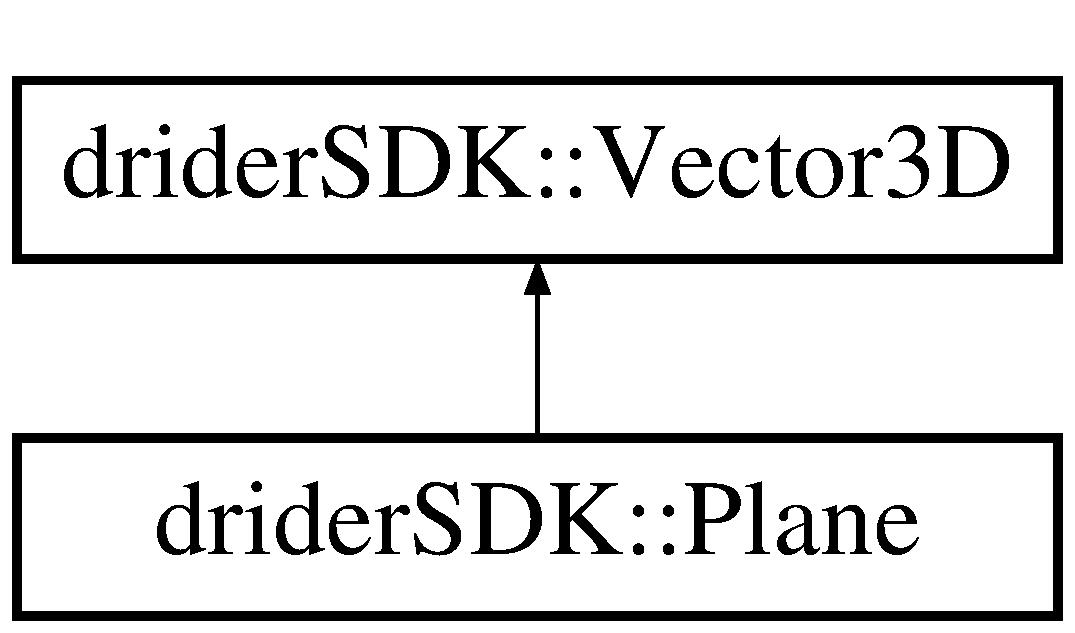
\includegraphics[height=2.000000cm]{classdrider_s_d_k_1_1_vector3_d}
\end{center}
\end{figure}
\subsection*{Public Member Functions}
\begin{DoxyCompactItemize}
\item 
\hyperlink{classdrider_s_d_k_1_1_vector3_d_a13d08e7ca2aea2687fc886140fd3e7cb}{Vector3D} ()
\item 
\hyperlink{classdrider_s_d_k_1_1_vector3_d_a69599690e85407589a6ac4f6dbe7454e}{Vector3D} (Math\+::\+F\+O\+R\+C\+E\+\_\+\+I\+N\+IT k)
\item 
\hyperlink{classdrider_s_d_k_1_1_vector3_d_a13783843ebb3807bbe1731e57bef3c1f}{Vector3D} (\hyperlink{classdrider_s_d_k_1_1_vector3_d}{Vector3D} \&\&V)=default
\item 
\hyperlink{classdrider_s_d_k_1_1_vector3_d_a6706fd9097922c155576146de3f51a67}{Vector3D} (const \hyperlink{classdrider_s_d_k_1_1_vector3_d}{Vector3D} \&V)
\item 
\hyperlink{classdrider_s_d_k_1_1_vector3_d_a7811eca35e237f48972788b59ea9b07e}{Vector3D} (float x, float y, float z)
\item 
\hyperlink{classdrider_s_d_k_1_1_vector3_d_af34c4e39b0fea97468aa1012bc842a8d}{$\sim$\+Vector3D} ()
\item 
float \hyperlink{classdrider_s_d_k_1_1_vector3_d_ac49c5b28ee95fbe6d7fae02f00008b6d}{dot} (const \hyperlink{classdrider_s_d_k_1_1_vector3_d}{Vector3D} \&B) const
\item 
\hyperlink{classdrider_s_d_k_1_1_vector3_d}{Vector3D} \hyperlink{classdrider_s_d_k_1_1_vector3_d_ae2338b1fbca5b81112571c81418eac5e}{cross} (const \hyperlink{classdrider_s_d_k_1_1_vector3_d}{Vector3D} \&B) const
\item 
float \hyperlink{classdrider_s_d_k_1_1_vector3_d_aa922725a227a655e4245a67b40840bb6}{length} () const
\item 
float \hyperlink{classdrider_s_d_k_1_1_vector3_d_a95efa15ddb5b55ab4278dc45e1da88e1}{length\+Sqr} () const
\item 
void \hyperlink{classdrider_s_d_k_1_1_vector3_d_afcec7f0ed8e1b080c1cdaf3d0cedac5c}{normalize} ()
\item 
float \hyperlink{classdrider_s_d_k_1_1_vector3_d_a77420a5cccfd611d38365dc9b19a7364}{distance} (const \hyperlink{classdrider_s_d_k_1_1_vector3_d}{Vector3D} \&other\+Vector) const
\item 
float \hyperlink{classdrider_s_d_k_1_1_vector3_d_a861d1e31856dabdc229c26b6fbab60a8}{distance\+Sqr} (const \hyperlink{classdrider_s_d_k_1_1_vector3_d}{Vector3D} \&other\+Vector) const
\item 
float \hyperlink{classdrider_s_d_k_1_1_vector3_d_a17428bbe32652edcba681b55e27853b2}{sqr\+Dist\+Segment} (const \hyperlink{classdrider_s_d_k_1_1_vector3_d}{Vector3D} \&pointA, const \hyperlink{classdrider_s_d_k_1_1_vector3_d}{Vector3D} \&pointB) const
\item 
float \& \hyperlink{classdrider_s_d_k_1_1_vector3_d_ac7f67c8043cc9f9d801a7e7a2f2580a7}{operator\mbox{[}$\,$\mbox{]}} (SizeT index)
\item 
const float \& \hyperlink{classdrider_s_d_k_1_1_vector3_d_a54c01f85259ba8f84eb37dcf1001e59e}{operator\mbox{[}$\,$\mbox{]}} (SizeT index) const
\item 
float \hyperlink{classdrider_s_d_k_1_1_vector3_d_a4681c3fae6e11a1bc33100f638a8bb25}{operator$\vert$} (const \hyperlink{classdrider_s_d_k_1_1_vector3_d}{Vector3D} \&B) const
\item 
\hyperlink{classdrider_s_d_k_1_1_vector3_d}{Vector3D} \hyperlink{classdrider_s_d_k_1_1_vector3_d_a174bcd0e5030b457337a74c90ab061fe}{operator$^\wedge$} (const \hyperlink{classdrider_s_d_k_1_1_vector3_d}{Vector3D} \&B) const
\item 
\mbox{\Hypertarget{classdrider_s_d_k_1_1_vector3_d_a6f290466b4c2583b0687861372bd6bd2}\label{classdrider_s_d_k_1_1_vector3_d_a6f290466b4c2583b0687861372bd6bd2}} 
\hyperlink{classdrider_s_d_k_1_1_vector3_d}{Vector3D} \& {\bfseries operator=} (const \hyperlink{classdrider_s_d_k_1_1_vector3_d}{Vector3D} \&A)
\item 
\mbox{\Hypertarget{classdrider_s_d_k_1_1_vector3_d_a070a52602fede494fe8001dbbcdb7b82}\label{classdrider_s_d_k_1_1_vector3_d_a070a52602fede494fe8001dbbcdb7b82}} 
\hyperlink{classdrider_s_d_k_1_1_vector3_d}{Vector3D} {\bfseries operator+} (const \hyperlink{classdrider_s_d_k_1_1_vector3_d}{Vector3D} \&A) const
\item 
\mbox{\Hypertarget{classdrider_s_d_k_1_1_vector3_d_ae5d5813d5376850d0a9a8c3f7af02c44}\label{classdrider_s_d_k_1_1_vector3_d_ae5d5813d5376850d0a9a8c3f7af02c44}} 
\hyperlink{classdrider_s_d_k_1_1_vector3_d}{Vector3D} \& {\bfseries operator+=} (const \hyperlink{classdrider_s_d_k_1_1_vector3_d}{Vector3D} \&A)
\item 
\mbox{\Hypertarget{classdrider_s_d_k_1_1_vector3_d_a04bdf7e8cb2ccc0b88dc521a6d5f0293}\label{classdrider_s_d_k_1_1_vector3_d_a04bdf7e8cb2ccc0b88dc521a6d5f0293}} 
\hyperlink{classdrider_s_d_k_1_1_vector3_d}{Vector3D} {\bfseries operator-\/} (const \hyperlink{classdrider_s_d_k_1_1_vector3_d}{Vector3D} \&A) const
\item 
\mbox{\Hypertarget{classdrider_s_d_k_1_1_vector3_d_aec4620baccb156f4e3fa55714fb6f447}\label{classdrider_s_d_k_1_1_vector3_d_aec4620baccb156f4e3fa55714fb6f447}} 
\hyperlink{classdrider_s_d_k_1_1_vector3_d}{Vector3D} \& {\bfseries operator-\/=} (const \hyperlink{classdrider_s_d_k_1_1_vector3_d}{Vector3D} \&A)
\item 
\mbox{\Hypertarget{classdrider_s_d_k_1_1_vector3_d_a01533415912b63ad5b9d63990b08414c}\label{classdrider_s_d_k_1_1_vector3_d_a01533415912b63ad5b9d63990b08414c}} 
\hyperlink{classdrider_s_d_k_1_1_vector3_d}{Vector3D} {\bfseries operator$\ast$} (const \hyperlink{classdrider_s_d_k_1_1_vector3_d}{Vector3D} \&A) const
\item 
\mbox{\Hypertarget{classdrider_s_d_k_1_1_vector3_d_a5fc6f6d5abad70a7ed4ec1a9f9b6bfe1}\label{classdrider_s_d_k_1_1_vector3_d_a5fc6f6d5abad70a7ed4ec1a9f9b6bfe1}} 
\hyperlink{classdrider_s_d_k_1_1_vector3_d}{Vector3D} \& {\bfseries operator$\ast$=} (const \hyperlink{classdrider_s_d_k_1_1_vector3_d}{Vector3D} \&A)
\item 
\mbox{\Hypertarget{classdrider_s_d_k_1_1_vector3_d_a63100babbbe1a36fe6dd0cacec94e3df}\label{classdrider_s_d_k_1_1_vector3_d_a63100babbbe1a36fe6dd0cacec94e3df}} 
\hyperlink{classdrider_s_d_k_1_1_vector3_d}{Vector3D} {\bfseries operator$\ast$} (const float scalar) const
\item 
\mbox{\Hypertarget{classdrider_s_d_k_1_1_vector3_d_ad621093d1d09f1ef187626624736a73e}\label{classdrider_s_d_k_1_1_vector3_d_ad621093d1d09f1ef187626624736a73e}} 
\hyperlink{classdrider_s_d_k_1_1_vector3_d}{Vector3D} \& {\bfseries operator$\ast$=} (const float scalar)
\item 
\mbox{\Hypertarget{classdrider_s_d_k_1_1_vector3_d_a65e02ff3b85e82e23818a77166befd46}\label{classdrider_s_d_k_1_1_vector3_d_a65e02ff3b85e82e23818a77166befd46}} 
\hyperlink{classdrider_s_d_k_1_1_vector3_d}{Vector3D} {\bfseries operator/} (const float scalar) const
\item 
\mbox{\Hypertarget{classdrider_s_d_k_1_1_vector3_d_adcd462b0ae22c8750c2bfc064d3cde5b}\label{classdrider_s_d_k_1_1_vector3_d_adcd462b0ae22c8750c2bfc064d3cde5b}} 
\hyperlink{classdrider_s_d_k_1_1_vector3_d}{Vector3D} \& {\bfseries operator/=} (const float scalar)
\item 
\mbox{\Hypertarget{classdrider_s_d_k_1_1_vector3_d_a0c6a7de13b40a5b976828a54d972884b}\label{classdrider_s_d_k_1_1_vector3_d_a0c6a7de13b40a5b976828a54d972884b}} 
bool {\bfseries operator==} (const \hyperlink{classdrider_s_d_k_1_1_vector3_d}{Vector3D} \&other\+Vector)
\item 
\mbox{\Hypertarget{classdrider_s_d_k_1_1_vector3_d_a388c35d03367a256738f5d99e99260b2}\label{classdrider_s_d_k_1_1_vector3_d_a388c35d03367a256738f5d99e99260b2}} 
bool {\bfseries operator!=} (const \hyperlink{classdrider_s_d_k_1_1_vector3_d}{Vector3D} \&other\+Vector)
\item 
\mbox{\Hypertarget{classdrider_s_d_k_1_1_vector3_d_a4b3922847be7defb6eef9a74746b0e31}\label{classdrider_s_d_k_1_1_vector3_d_a4b3922847be7defb6eef9a74746b0e31}} 
\hyperlink{classdrider_s_d_k_1_1_vector3_d}{Vector3D} {\bfseries operator-\/} () const
\end{DoxyCompactItemize}
\subsection*{Public Attributes}
\begin{DoxyCompactItemize}
\item 
\mbox{\Hypertarget{classdrider_s_d_k_1_1_vector3_d_a065a234f94a65617b2a62943f1b7ca1d}\label{classdrider_s_d_k_1_1_vector3_d_a065a234f94a65617b2a62943f1b7ca1d}} 
\begin{tabbing}
xx\=xx\=xx\=xx\=xx\=xx\=xx\=xx\=xx\=\kill
union \{\\
\mbox{\Hypertarget{uniondrider_s_d_k_1_1_vector3_d_1_1_0D20_ac6552a061d1b9b976df18a94973c54b1}\label{uniondrider_s_d_k_1_1_vector3_d_1_1_0D20_ac6552a061d1b9b976df18a94973c54b1}} 
\>struct \{\\
\>\>float {\bfseries x}\\
\>\>float {\bfseries y}\\
\>\>float {\bfseries z}\\
\>\} \\
\>float {\bfseries data} \mbox{[}3\mbox{]}\\
\}; \\

\end{tabbing}\end{DoxyCompactItemize}


\subsection{Constructor \& Destructor Documentation}
\mbox{\Hypertarget{classdrider_s_d_k_1_1_vector3_d_a13d08e7ca2aea2687fc886140fd3e7cb}\label{classdrider_s_d_k_1_1_vector3_d_a13d08e7ca2aea2687fc886140fd3e7cb}} 
\index{drider\+S\+D\+K\+::\+Vector3D@{drider\+S\+D\+K\+::\+Vector3D}!Vector3D@{Vector3D}}
\index{Vector3D@{Vector3D}!drider\+S\+D\+K\+::\+Vector3D@{drider\+S\+D\+K\+::\+Vector3D}}
\subsubsection{\texorpdfstring{Vector3\+D()}{Vector3D()}\hspace{0.1cm}{\footnotesize\ttfamily [1/5]}}
{\footnotesize\ttfamily drider\+S\+D\+K\+::\+Vector3\+D\+::\+Vector3D (\begin{DoxyParamCaption}{ }\end{DoxyParamCaption})}

Default constructor \mbox{\Hypertarget{classdrider_s_d_k_1_1_vector3_d_a69599690e85407589a6ac4f6dbe7454e}\label{classdrider_s_d_k_1_1_vector3_d_a69599690e85407589a6ac4f6dbe7454e}} 
\index{drider\+S\+D\+K\+::\+Vector3D@{drider\+S\+D\+K\+::\+Vector3D}!Vector3D@{Vector3D}}
\index{Vector3D@{Vector3D}!drider\+S\+D\+K\+::\+Vector3D@{drider\+S\+D\+K\+::\+Vector3D}}
\subsubsection{\texorpdfstring{Vector3\+D()}{Vector3D()}\hspace{0.1cm}{\footnotesize\ttfamily [2/5]}}
{\footnotesize\ttfamily drider\+S\+D\+K\+::\+Vector3\+D\+::\+Vector3D (\begin{DoxyParamCaption}\item[{Math\+::\+F\+O\+R\+C\+E\+\_\+\+I\+N\+IT}]{k }\end{DoxyParamCaption})\hspace{0.3cm}{\ttfamily [explicit]}}

Default constructor


\begin{DoxyParams}{Parameters}
{\em k} & Values are initialized with 0. \\
\hline
\end{DoxyParams}
\mbox{\Hypertarget{classdrider_s_d_k_1_1_vector3_d_a13783843ebb3807bbe1731e57bef3c1f}\label{classdrider_s_d_k_1_1_vector3_d_a13783843ebb3807bbe1731e57bef3c1f}} 
\index{drider\+S\+D\+K\+::\+Vector3D@{drider\+S\+D\+K\+::\+Vector3D}!Vector3D@{Vector3D}}
\index{Vector3D@{Vector3D}!drider\+S\+D\+K\+::\+Vector3D@{drider\+S\+D\+K\+::\+Vector3D}}
\subsubsection{\texorpdfstring{Vector3\+D()}{Vector3D()}\hspace{0.1cm}{\footnotesize\ttfamily [3/5]}}
{\footnotesize\ttfamily drider\+S\+D\+K\+::\+Vector3\+D\+::\+Vector3D (\begin{DoxyParamCaption}\item[{\hyperlink{classdrider_s_d_k_1_1_vector3_d}{Vector3D} \&\&}]{V }\end{DoxyParamCaption})\hspace{0.3cm}{\ttfamily [default]}}

Move constructor \mbox{\Hypertarget{classdrider_s_d_k_1_1_vector3_d_a6706fd9097922c155576146de3f51a67}\label{classdrider_s_d_k_1_1_vector3_d_a6706fd9097922c155576146de3f51a67}} 
\index{drider\+S\+D\+K\+::\+Vector3D@{drider\+S\+D\+K\+::\+Vector3D}!Vector3D@{Vector3D}}
\index{Vector3D@{Vector3D}!drider\+S\+D\+K\+::\+Vector3D@{drider\+S\+D\+K\+::\+Vector3D}}
\subsubsection{\texorpdfstring{Vector3\+D()}{Vector3D()}\hspace{0.1cm}{\footnotesize\ttfamily [4/5]}}
{\footnotesize\ttfamily drider\+S\+D\+K\+::\+Vector3\+D\+::\+Vector3D (\begin{DoxyParamCaption}\item[{const \hyperlink{classdrider_s_d_k_1_1_vector3_d}{Vector3D} \&}]{V }\end{DoxyParamCaption})}

Copy constructor \mbox{\Hypertarget{classdrider_s_d_k_1_1_vector3_d_a7811eca35e237f48972788b59ea9b07e}\label{classdrider_s_d_k_1_1_vector3_d_a7811eca35e237f48972788b59ea9b07e}} 
\index{drider\+S\+D\+K\+::\+Vector3D@{drider\+S\+D\+K\+::\+Vector3D}!Vector3D@{Vector3D}}
\index{Vector3D@{Vector3D}!drider\+S\+D\+K\+::\+Vector3D@{drider\+S\+D\+K\+::\+Vector3D}}
\subsubsection{\texorpdfstring{Vector3\+D()}{Vector3D()}\hspace{0.1cm}{\footnotesize\ttfamily [5/5]}}
{\footnotesize\ttfamily drider\+S\+D\+K\+::\+Vector3\+D\+::\+Vector3D (\begin{DoxyParamCaption}\item[{float}]{x,  }\item[{float}]{y,  }\item[{float}]{z }\end{DoxyParamCaption})}

Initialize constructor with values.


\begin{DoxyParams}{Parameters}
{\em x} & The x value of the vector\\
\hline
{\em y} & The y value of the vector\\
\hline
{\em z} & The z value of the vector \\
\hline
\end{DoxyParams}
\mbox{\Hypertarget{classdrider_s_d_k_1_1_vector3_d_af34c4e39b0fea97468aa1012bc842a8d}\label{classdrider_s_d_k_1_1_vector3_d_af34c4e39b0fea97468aa1012bc842a8d}} 
\index{drider\+S\+D\+K\+::\+Vector3D@{drider\+S\+D\+K\+::\+Vector3D}!````~Vector3D@{$\sim$\+Vector3D}}
\index{````~Vector3D@{$\sim$\+Vector3D}!drider\+S\+D\+K\+::\+Vector3D@{drider\+S\+D\+K\+::\+Vector3D}}
\subsubsection{\texorpdfstring{$\sim$\+Vector3\+D()}{~Vector3D()}}
{\footnotesize\ttfamily drider\+S\+D\+K\+::\+Vector3\+D\+::$\sim$\+Vector3D (\begin{DoxyParamCaption}{ }\end{DoxyParamCaption})}

Default destructor 

\subsection{Member Function Documentation}
\mbox{\Hypertarget{classdrider_s_d_k_1_1_vector3_d_ae2338b1fbca5b81112571c81418eac5e}\label{classdrider_s_d_k_1_1_vector3_d_ae2338b1fbca5b81112571c81418eac5e}} 
\index{drider\+S\+D\+K\+::\+Vector3D@{drider\+S\+D\+K\+::\+Vector3D}!cross@{cross}}
\index{cross@{cross}!drider\+S\+D\+K\+::\+Vector3D@{drider\+S\+D\+K\+::\+Vector3D}}
\subsubsection{\texorpdfstring{cross()}{cross()}}
{\footnotesize\ttfamily \hyperlink{classdrider_s_d_k_1_1_vector3_d}{Vector3D} drider\+S\+D\+K\+::\+Vector3\+D\+::cross (\begin{DoxyParamCaption}\item[{const \hyperlink{classdrider_s_d_k_1_1_vector3_d}{Vector3D} \&}]{B }\end{DoxyParamCaption}) const}

Computes the cross product between this vector and the vector parameter. This operatios is N\+OT commutative.


\begin{DoxyParams}{Parameters}
{\em B} & The vector against which the cross product is calculated. B (vector parameter) is the rigth value of operation AxB\\
\hline
\end{DoxyParams}
\begin{DoxyReturn}{Returns}
Result vector of the cross product 
\end{DoxyReturn}
\mbox{\Hypertarget{classdrider_s_d_k_1_1_vector3_d_a77420a5cccfd611d38365dc9b19a7364}\label{classdrider_s_d_k_1_1_vector3_d_a77420a5cccfd611d38365dc9b19a7364}} 
\index{drider\+S\+D\+K\+::\+Vector3D@{drider\+S\+D\+K\+::\+Vector3D}!distance@{distance}}
\index{distance@{distance}!drider\+S\+D\+K\+::\+Vector3D@{drider\+S\+D\+K\+::\+Vector3D}}
\subsubsection{\texorpdfstring{distance()}{distance()}}
{\footnotesize\ttfamily float drider\+S\+D\+K\+::\+Vector3\+D\+::distance (\begin{DoxyParamCaption}\item[{const \hyperlink{classdrider_s_d_k_1_1_vector3_d}{Vector3D} \&}]{other\+Vector }\end{DoxyParamCaption}) const}

Computes the distance between two vectors.


\begin{DoxyParams}{Parameters}
{\em scalar} & Vector to calculate the distance\\
\hline
\end{DoxyParams}
\begin{DoxyReturn}{Returns}
Distance 
\end{DoxyReturn}
\mbox{\Hypertarget{classdrider_s_d_k_1_1_vector3_d_a861d1e31856dabdc229c26b6fbab60a8}\label{classdrider_s_d_k_1_1_vector3_d_a861d1e31856dabdc229c26b6fbab60a8}} 
\index{drider\+S\+D\+K\+::\+Vector3D@{drider\+S\+D\+K\+::\+Vector3D}!distance\+Sqr@{distance\+Sqr}}
\index{distance\+Sqr@{distance\+Sqr}!drider\+S\+D\+K\+::\+Vector3D@{drider\+S\+D\+K\+::\+Vector3D}}
\subsubsection{\texorpdfstring{distance\+Sqr()}{distanceSqr()}}
{\footnotesize\ttfamily float drider\+S\+D\+K\+::\+Vector3\+D\+::distance\+Sqr (\begin{DoxyParamCaption}\item[{const \hyperlink{classdrider_s_d_k_1_1_vector3_d}{Vector3D} \&}]{other\+Vector }\end{DoxyParamCaption}) const}

Computes the squared distance between two vectors.


\begin{DoxyParams}{Parameters}
{\em scalar} & Vector to calculate the distance\\
\hline
\end{DoxyParams}
\begin{DoxyReturn}{Returns}
Distance 
\end{DoxyReturn}
\mbox{\Hypertarget{classdrider_s_d_k_1_1_vector3_d_ac49c5b28ee95fbe6d7fae02f00008b6d}\label{classdrider_s_d_k_1_1_vector3_d_ac49c5b28ee95fbe6d7fae02f00008b6d}} 
\index{drider\+S\+D\+K\+::\+Vector3D@{drider\+S\+D\+K\+::\+Vector3D}!dot@{dot}}
\index{dot@{dot}!drider\+S\+D\+K\+::\+Vector3D@{drider\+S\+D\+K\+::\+Vector3D}}
\subsubsection{\texorpdfstring{dot()}{dot()}}
{\footnotesize\ttfamily float drider\+S\+D\+K\+::\+Vector3\+D\+::dot (\begin{DoxyParamCaption}\item[{const \hyperlink{classdrider_s_d_k_1_1_vector3_d}{Vector3D} \&}]{B }\end{DoxyParamCaption}) const}

Computes the dot product between this vector and the vector parameter. This operatios is commutative.


\begin{DoxyParams}{Parameters}
{\em B} & The vector against which the dot product is calculated.\\
\hline
\end{DoxyParams}
\begin{DoxyReturn}{Returns}
The sum of the products of the corresponding entries of the vectors. 
\end{DoxyReturn}
\mbox{\Hypertarget{classdrider_s_d_k_1_1_vector3_d_aa922725a227a655e4245a67b40840bb6}\label{classdrider_s_d_k_1_1_vector3_d_aa922725a227a655e4245a67b40840bb6}} 
\index{drider\+S\+D\+K\+::\+Vector3D@{drider\+S\+D\+K\+::\+Vector3D}!length@{length}}
\index{length@{length}!drider\+S\+D\+K\+::\+Vector3D@{drider\+S\+D\+K\+::\+Vector3D}}
\subsubsection{\texorpdfstring{length()}{length()}}
{\footnotesize\ttfamily float drider\+S\+D\+K\+::\+Vector3\+D\+::length (\begin{DoxyParamCaption}{ }\end{DoxyParamCaption}) const}

Computes the length of this vector.

\begin{DoxyReturn}{Returns}
The length (or \char`\"{}size\char`\"{}) of the vector. 
\end{DoxyReturn}
\mbox{\Hypertarget{classdrider_s_d_k_1_1_vector3_d_a95efa15ddb5b55ab4278dc45e1da88e1}\label{classdrider_s_d_k_1_1_vector3_d_a95efa15ddb5b55ab4278dc45e1da88e1}} 
\index{drider\+S\+D\+K\+::\+Vector3D@{drider\+S\+D\+K\+::\+Vector3D}!length\+Sqr@{length\+Sqr}}
\index{length\+Sqr@{length\+Sqr}!drider\+S\+D\+K\+::\+Vector3D@{drider\+S\+D\+K\+::\+Vector3D}}
\subsubsection{\texorpdfstring{length\+Sqr()}{lengthSqr()}}
{\footnotesize\ttfamily float drider\+S\+D\+K\+::\+Vector3\+D\+::length\+Sqr (\begin{DoxyParamCaption}{ }\end{DoxyParamCaption}) const}

Computes the squared length of this vector.

\begin{DoxyReturn}{Returns}
The length (or \char`\"{}size\char`\"{}) of the vector squared. 
\end{DoxyReturn}
\mbox{\Hypertarget{classdrider_s_d_k_1_1_vector3_d_afcec7f0ed8e1b080c1cdaf3d0cedac5c}\label{classdrider_s_d_k_1_1_vector3_d_afcec7f0ed8e1b080c1cdaf3d0cedac5c}} 
\index{drider\+S\+D\+K\+::\+Vector3D@{drider\+S\+D\+K\+::\+Vector3D}!normalize@{normalize}}
\index{normalize@{normalize}!drider\+S\+D\+K\+::\+Vector3D@{drider\+S\+D\+K\+::\+Vector3D}}
\subsubsection{\texorpdfstring{normalize()}{normalize()}}
{\footnotesize\ttfamily void drider\+S\+D\+K\+::\+Vector3\+D\+::normalize (\begin{DoxyParamCaption}{ }\end{DoxyParamCaption})}

Normalize the vector. \mbox{\Hypertarget{classdrider_s_d_k_1_1_vector3_d_ac7f67c8043cc9f9d801a7e7a2f2580a7}\label{classdrider_s_d_k_1_1_vector3_d_ac7f67c8043cc9f9d801a7e7a2f2580a7}} 
\index{drider\+S\+D\+K\+::\+Vector3D@{drider\+S\+D\+K\+::\+Vector3D}!operator\mbox{[}\mbox{]}@{operator[]}}
\index{operator\mbox{[}\mbox{]}@{operator[]}!drider\+S\+D\+K\+::\+Vector3D@{drider\+S\+D\+K\+::\+Vector3D}}
\subsubsection{\texorpdfstring{operator[]()}{operator[]()}\hspace{0.1cm}{\footnotesize\ttfamily [1/2]}}
{\footnotesize\ttfamily float \& drider\+S\+D\+K\+::\+Vector3\+D\+::operator\mbox{[}$\,$\mbox{]} (\begin{DoxyParamCaption}\item[{SizeT}]{index }\end{DoxyParamCaption})}

Gets a reference to the specified element from the vector.


\begin{DoxyParams}{Parameters}
{\em index} & The index of the element.\\
\hline
\end{DoxyParams}
\begin{DoxyReturn}{Returns}
A const reference to the element at the \mbox{[}index\mbox{]} position.
\end{DoxyReturn}

\begin{DoxyExceptions}{Exceptions}
{\em out\+\_\+of\+\_\+range} & If the index is greater than number of elements in the vector. \\
\hline
\end{DoxyExceptions}
\mbox{\Hypertarget{classdrider_s_d_k_1_1_vector3_d_a54c01f85259ba8f84eb37dcf1001e59e}\label{classdrider_s_d_k_1_1_vector3_d_a54c01f85259ba8f84eb37dcf1001e59e}} 
\index{drider\+S\+D\+K\+::\+Vector3D@{drider\+S\+D\+K\+::\+Vector3D}!operator\mbox{[}\mbox{]}@{operator[]}}
\index{operator\mbox{[}\mbox{]}@{operator[]}!drider\+S\+D\+K\+::\+Vector3D@{drider\+S\+D\+K\+::\+Vector3D}}
\subsubsection{\texorpdfstring{operator[]()}{operator[]()}\hspace{0.1cm}{\footnotesize\ttfamily [2/2]}}
{\footnotesize\ttfamily const float \& drider\+S\+D\+K\+::\+Vector3\+D\+::operator\mbox{[}$\,$\mbox{]} (\begin{DoxyParamCaption}\item[{SizeT}]{index }\end{DoxyParamCaption}) const}

Gets a reference to the specified element from the vector.


\begin{DoxyParams}{Parameters}
{\em index} & The index of the element.\\
\hline
\end{DoxyParams}
\begin{DoxyReturn}{Returns}
A const reference to the element at the \mbox{[}index\mbox{]} position.
\end{DoxyReturn}

\begin{DoxyExceptions}{Exceptions}
{\em out\+\_\+of\+\_\+range} & If the index is greater than number of elements in the vector. \\
\hline
\end{DoxyExceptions}
\mbox{\Hypertarget{classdrider_s_d_k_1_1_vector3_d_a174bcd0e5030b457337a74c90ab061fe}\label{classdrider_s_d_k_1_1_vector3_d_a174bcd0e5030b457337a74c90ab061fe}} 
\index{drider\+S\+D\+K\+::\+Vector3D@{drider\+S\+D\+K\+::\+Vector3D}!operator$^\wedge$@{operator$^\wedge$}}
\index{operator$^\wedge$@{operator$^\wedge$}!drider\+S\+D\+K\+::\+Vector3D@{drider\+S\+D\+K\+::\+Vector3D}}
\subsubsection{\texorpdfstring{operator$^\wedge$()}{operator^()}}
{\footnotesize\ttfamily \hyperlink{classdrider_s_d_k_1_1_vector3_d}{Vector3D} drider\+S\+D\+K\+::\+Vector3\+D\+::operator$^\wedge$ (\begin{DoxyParamCaption}\item[{const \hyperlink{classdrider_s_d_k_1_1_vector3_d}{Vector3D} \&}]{B }\end{DoxyParamCaption}) const}

Computes the cross product between this vector and the vector parameter. This operatios is N\+OT commutative.


\begin{DoxyParams}{Parameters}
{\em B} & The vector against which the cross product is calculated. B (vector parameter) is the rigth value of operation AxB\\
\hline
\end{DoxyParams}
\begin{DoxyReturn}{Returns}
Result vector of the cross product 
\end{DoxyReturn}
\mbox{\Hypertarget{classdrider_s_d_k_1_1_vector3_d_a4681c3fae6e11a1bc33100f638a8bb25}\label{classdrider_s_d_k_1_1_vector3_d_a4681c3fae6e11a1bc33100f638a8bb25}} 
\index{drider\+S\+D\+K\+::\+Vector3D@{drider\+S\+D\+K\+::\+Vector3D}!operator\texttt{"|}@{operator\texttt{"|}}}
\index{operator\texttt{"|}@{operator\texttt{"|}}!drider\+S\+D\+K\+::\+Vector3D@{drider\+S\+D\+K\+::\+Vector3D}}
\subsubsection{\texorpdfstring{operator\texttt{"|}()}{operator|()}}
{\footnotesize\ttfamily float drider\+S\+D\+K\+::\+Vector3\+D\+::operator$\vert$ (\begin{DoxyParamCaption}\item[{const \hyperlink{classdrider_s_d_k_1_1_vector3_d}{Vector3D} \&}]{B }\end{DoxyParamCaption}) const}

Computes the dot product between this vector and the vector parameter. This operatios is commutative.


\begin{DoxyParams}{Parameters}
{\em B} & The vector against which the dot product is calculated.\\
\hline
\end{DoxyParams}
\begin{DoxyReturn}{Returns}
The sum of the products of the corresponding entries of the vectors. 
\end{DoxyReturn}
\mbox{\Hypertarget{classdrider_s_d_k_1_1_vector3_d_a17428bbe32652edcba681b55e27853b2}\label{classdrider_s_d_k_1_1_vector3_d_a17428bbe32652edcba681b55e27853b2}} 
\index{drider\+S\+D\+K\+::\+Vector3D@{drider\+S\+D\+K\+::\+Vector3D}!sqr\+Dist\+Segment@{sqr\+Dist\+Segment}}
\index{sqr\+Dist\+Segment@{sqr\+Dist\+Segment}!drider\+S\+D\+K\+::\+Vector3D@{drider\+S\+D\+K\+::\+Vector3D}}
\subsubsection{\texorpdfstring{sqr\+Dist\+Segment()}{sqrDistSegment()}}
{\footnotesize\ttfamily float drider\+S\+D\+K\+::\+Vector3\+D\+::sqr\+Dist\+Segment (\begin{DoxyParamCaption}\item[{const \hyperlink{classdrider_s_d_k_1_1_vector3_d}{Vector3D} \&}]{pointA,  }\item[{const \hyperlink{classdrider_s_d_k_1_1_vector3_d}{Vector3D} \&}]{pointB }\end{DoxyParamCaption}) const}

Computes the squared distance between a point and a segment.


\begin{DoxyParams}{Parameters}
{\em pointA} & Point a of the segment.\\
\hline
{\em pointB} & Point b of the segment.\\
\hline
\end{DoxyParams}
\begin{DoxyReturn}{Returns}
Distance 
\end{DoxyReturn}


The documentation for this class was generated from the following files\+:\begin{DoxyCompactItemize}
\item 
C\+:/\+Users/\+Francisco/source/repos/\+Drider-\/\+Engine/\+Math/\+Include/dr\+\_\+vector3d.\+h\item 
C\+:/\+Users/\+Francisco/source/repos/\+Drider-\/\+Engine/\+Math/\+Source/dr\+\_\+vector3d.\+cpp\end{DoxyCompactItemize}

\hypertarget{classdrider_s_d_k_1_1_vector4_d}{}\section{drider\+S\+DK\+:\+:Vector4D Class Reference}
\label{classdrider_s_d_k_1_1_vector4_d}\index{drider\+S\+D\+K\+::\+Vector4D@{drider\+S\+D\+K\+::\+Vector4D}}
\subsection*{Public Member Functions}
\begin{DoxyCompactItemize}
\item 
\hyperlink{classdrider_s_d_k_1_1_vector4_d_af010e3865425352f4ab21df1144cffcf}{Vector4D} ()
\item 
\hyperlink{classdrider_s_d_k_1_1_vector4_d_aeff81eebdc91a9adfb959a66767a6281}{Vector4D} (Math\+::\+F\+O\+R\+C\+E\+\_\+\+I\+N\+IT k)
\item 
\hyperlink{classdrider_s_d_k_1_1_vector4_d_a2cd19b93232ceec414455d18472fc438}{Vector4D} (\hyperlink{classdrider_s_d_k_1_1_vector4_d}{Vector4D} \&\&V)=default
\item 
\hyperlink{classdrider_s_d_k_1_1_vector4_d_a985e70f8324e74ea261429d9ed0d8175}{Vector4D} (const \hyperlink{classdrider_s_d_k_1_1_vector4_d}{Vector4D} \&V)
\item 
\hyperlink{classdrider_s_d_k_1_1_vector4_d_a942402976cfe8940344b2e8d0367338e}{Vector4D} (float x, float y, float z, float w)
\item 
\hyperlink{classdrider_s_d_k_1_1_vector4_d_ae01427a60f8ea96ac706e8d313503d87}{$\sim$\+Vector4D} ()
\item 
float \hyperlink{classdrider_s_d_k_1_1_vector4_d_aa8d1f7fff12b2ac119cadc3938652fed}{dot} (const \hyperlink{classdrider_s_d_k_1_1_vector4_d}{Vector4D} \&B) const
\item 
\hyperlink{classdrider_s_d_k_1_1_vector4_d}{Vector4D} \hyperlink{classdrider_s_d_k_1_1_vector4_d_a81812e2af1876abb13a489f5264d9515}{cross} (const \hyperlink{classdrider_s_d_k_1_1_vector4_d}{Vector4D} \&B) const
\item 
float \hyperlink{classdrider_s_d_k_1_1_vector4_d_acef00dfefbd4491c7467468e7cb4c8c3}{length} () const
\item 
float \hyperlink{classdrider_s_d_k_1_1_vector4_d_a1ddcf3265baa39efedaa78e650ecabc0}{length\+Sqr} () const
\item 
void \hyperlink{classdrider_s_d_k_1_1_vector4_d_af833f447b91791df7d2a153bf77e127b}{normalize} ()
\item 
float \hyperlink{classdrider_s_d_k_1_1_vector4_d_a3aa1ea1f8fd24f6a1bc5475158c4ded7}{distance} (const \hyperlink{classdrider_s_d_k_1_1_vector4_d}{Vector4D} \&other\+Vector) const
\item 
float \hyperlink{classdrider_s_d_k_1_1_vector4_d_ae470e090d587784df55ed6dce94f57fc}{distance\+Sqr} (const \hyperlink{classdrider_s_d_k_1_1_vector4_d}{Vector4D} \&other\+Vector) const
\item 
float \& \hyperlink{classdrider_s_d_k_1_1_vector4_d_a22777557bf66b8adeb50f24f2943fc66}{operator\mbox{[}$\,$\mbox{]}} (SizeT index)
\item 
const float \& \hyperlink{classdrider_s_d_k_1_1_vector4_d_a6da3ce7013d8b4fef78986433af25971}{operator\mbox{[}$\,$\mbox{]}} (SizeT index) const
\item 
float \hyperlink{classdrider_s_d_k_1_1_vector4_d_a40c293b7041c65fd20f8741b4c3c312d}{operator$\vert$} (const \hyperlink{classdrider_s_d_k_1_1_vector4_d}{Vector4D} \&B) const
\item 
\hyperlink{classdrider_s_d_k_1_1_vector4_d}{Vector4D} \hyperlink{classdrider_s_d_k_1_1_vector4_d_ae6ce7f847b9c2aaa07ba0e992d189587}{operator$^\wedge$} (const \hyperlink{classdrider_s_d_k_1_1_vector4_d}{Vector4D} \&B) const
\item 
\mbox{\Hypertarget{classdrider_s_d_k_1_1_vector4_d_a98eb14acc45ecbb0214fdaa25923aa9e}\label{classdrider_s_d_k_1_1_vector4_d_a98eb14acc45ecbb0214fdaa25923aa9e}} 
\hyperlink{classdrider_s_d_k_1_1_vector4_d}{Vector4D} \& {\bfseries operator=} (const \hyperlink{classdrider_s_d_k_1_1_vector4_d}{Vector4D} \&A)
\item 
\mbox{\Hypertarget{classdrider_s_d_k_1_1_vector4_d_a2c7fbcc833cfa0fb776a9231434293d0}\label{classdrider_s_d_k_1_1_vector4_d_a2c7fbcc833cfa0fb776a9231434293d0}} 
\hyperlink{classdrider_s_d_k_1_1_vector4_d}{Vector4D} {\bfseries operator+} (const \hyperlink{classdrider_s_d_k_1_1_vector4_d}{Vector4D} \&A) const
\item 
\mbox{\Hypertarget{classdrider_s_d_k_1_1_vector4_d_afb27b2c43a38df5767f1e0a9d2b77fc7}\label{classdrider_s_d_k_1_1_vector4_d_afb27b2c43a38df5767f1e0a9d2b77fc7}} 
\hyperlink{classdrider_s_d_k_1_1_vector4_d}{Vector4D} \& {\bfseries operator+=} (const \hyperlink{classdrider_s_d_k_1_1_vector4_d}{Vector4D} \&A)
\item 
\mbox{\Hypertarget{classdrider_s_d_k_1_1_vector4_d_a1f3b703db359083ab5061689b4721b9f}\label{classdrider_s_d_k_1_1_vector4_d_a1f3b703db359083ab5061689b4721b9f}} 
\hyperlink{classdrider_s_d_k_1_1_vector4_d}{Vector4D} {\bfseries operator-\/} (const \hyperlink{classdrider_s_d_k_1_1_vector4_d}{Vector4D} \&A) const
\item 
\mbox{\Hypertarget{classdrider_s_d_k_1_1_vector4_d_ac2b73c4fb5009b248229b08bbf8a7162}\label{classdrider_s_d_k_1_1_vector4_d_ac2b73c4fb5009b248229b08bbf8a7162}} 
\hyperlink{classdrider_s_d_k_1_1_vector4_d}{Vector4D} \& {\bfseries operator-\/=} (const \hyperlink{classdrider_s_d_k_1_1_vector4_d}{Vector4D} \&A)
\item 
\mbox{\Hypertarget{classdrider_s_d_k_1_1_vector4_d_a50b937f5430ad9086947dc109f226ef7}\label{classdrider_s_d_k_1_1_vector4_d_a50b937f5430ad9086947dc109f226ef7}} 
\hyperlink{classdrider_s_d_k_1_1_vector4_d}{Vector4D} {\bfseries operator$\ast$} (const \hyperlink{classdrider_s_d_k_1_1_vector4_d}{Vector4D} \&A) const
\item 
\mbox{\Hypertarget{classdrider_s_d_k_1_1_vector4_d_acc68d94661de25b6fc1f98ef8b303f93}\label{classdrider_s_d_k_1_1_vector4_d_acc68d94661de25b6fc1f98ef8b303f93}} 
\hyperlink{classdrider_s_d_k_1_1_vector4_d}{Vector4D} \& {\bfseries operator$\ast$=} (const \hyperlink{classdrider_s_d_k_1_1_vector4_d}{Vector4D} \&A)
\item 
\mbox{\Hypertarget{classdrider_s_d_k_1_1_vector4_d_a4122358589fc92de558c0b779be5859e}\label{classdrider_s_d_k_1_1_vector4_d_a4122358589fc92de558c0b779be5859e}} 
\hyperlink{classdrider_s_d_k_1_1_vector4_d}{Vector4D} {\bfseries operator$\ast$} (const float scalar) const
\item 
\mbox{\Hypertarget{classdrider_s_d_k_1_1_vector4_d_a3b821c9a44e6f57528f9351405bcf09d}\label{classdrider_s_d_k_1_1_vector4_d_a3b821c9a44e6f57528f9351405bcf09d}} 
\hyperlink{classdrider_s_d_k_1_1_vector4_d}{Vector4D} \& {\bfseries operator$\ast$=} (const float scalar)
\item 
\mbox{\Hypertarget{classdrider_s_d_k_1_1_vector4_d_a3ffbdf72847c8bdc042330d33c354a4c}\label{classdrider_s_d_k_1_1_vector4_d_a3ffbdf72847c8bdc042330d33c354a4c}} 
\hyperlink{classdrider_s_d_k_1_1_vector4_d}{Vector4D} {\bfseries operator/} (const float scalar) const
\item 
\mbox{\Hypertarget{classdrider_s_d_k_1_1_vector4_d_a83cdf9b4edc3de5feb89d7be90addd9a}\label{classdrider_s_d_k_1_1_vector4_d_a83cdf9b4edc3de5feb89d7be90addd9a}} 
\hyperlink{classdrider_s_d_k_1_1_vector4_d}{Vector4D} \& {\bfseries operator/=} (const float scalar)
\item 
\mbox{\Hypertarget{classdrider_s_d_k_1_1_vector4_d_a6c11c3389e6fa6cb3bbbc293b14806d8}\label{classdrider_s_d_k_1_1_vector4_d_a6c11c3389e6fa6cb3bbbc293b14806d8}} 
bool {\bfseries operator==} (const \hyperlink{classdrider_s_d_k_1_1_vector4_d}{Vector4D} \&other\+Vector)
\item 
\mbox{\Hypertarget{classdrider_s_d_k_1_1_vector4_d_a9a64a39e5a47327493b4c3cb9ca25434}\label{classdrider_s_d_k_1_1_vector4_d_a9a64a39e5a47327493b4c3cb9ca25434}} 
bool {\bfseries operator!=} (const \hyperlink{classdrider_s_d_k_1_1_vector4_d}{Vector4D} \&other\+Vector)
\item 
\mbox{\Hypertarget{classdrider_s_d_k_1_1_vector4_d_a2e055397526cc3a8980533c80729a899}\label{classdrider_s_d_k_1_1_vector4_d_a2e055397526cc3a8980533c80729a899}} 
\hyperlink{classdrider_s_d_k_1_1_vector4_d}{Vector4D} {\bfseries operator-\/} () const
\end{DoxyCompactItemize}
\subsection*{Public Attributes}
\begin{DoxyCompactItemize}
\item 
\mbox{\Hypertarget{classdrider_s_d_k_1_1_vector4_d_a3c6a9cbc294493a04d0cef1aa6d0eb2e}\label{classdrider_s_d_k_1_1_vector4_d_a3c6a9cbc294493a04d0cef1aa6d0eb2e}} 
\begin{tabbing}
xx\=xx\=xx\=xx\=xx\=xx\=xx\=xx\=xx\=\kill
union \{\\
\mbox{\Hypertarget{uniondrider_s_d_k_1_1_vector4_d_1_1_0D24_a60fc399dd2e2b657c951b09a4104884d}\label{uniondrider_s_d_k_1_1_vector4_d_1_1_0D24_a60fc399dd2e2b657c951b09a4104884d}} 
\>struct \{\\
\>\>float {\bfseries x}\\
\>\>float {\bfseries y}\\
\>\>float {\bfseries z}\\
\>\>float {\bfseries w}\\
\>\} \\
\>float {\bfseries data} \mbox{[}4\mbox{]}\\
\}; \\

\end{tabbing}\end{DoxyCompactItemize}


\subsection{Constructor \& Destructor Documentation}
\mbox{\Hypertarget{classdrider_s_d_k_1_1_vector4_d_af010e3865425352f4ab21df1144cffcf}\label{classdrider_s_d_k_1_1_vector4_d_af010e3865425352f4ab21df1144cffcf}} 
\index{drider\+S\+D\+K\+::\+Vector4D@{drider\+S\+D\+K\+::\+Vector4D}!Vector4D@{Vector4D}}
\index{Vector4D@{Vector4D}!drider\+S\+D\+K\+::\+Vector4D@{drider\+S\+D\+K\+::\+Vector4D}}
\subsubsection{\texorpdfstring{Vector4\+D()}{Vector4D()}\hspace{0.1cm}{\footnotesize\ttfamily [1/5]}}
{\footnotesize\ttfamily drider\+S\+D\+K\+::\+Vector4\+D\+::\+Vector4D (\begin{DoxyParamCaption}{ }\end{DoxyParamCaption})}

Default constructor \mbox{\Hypertarget{classdrider_s_d_k_1_1_vector4_d_aeff81eebdc91a9adfb959a66767a6281}\label{classdrider_s_d_k_1_1_vector4_d_aeff81eebdc91a9adfb959a66767a6281}} 
\index{drider\+S\+D\+K\+::\+Vector4D@{drider\+S\+D\+K\+::\+Vector4D}!Vector4D@{Vector4D}}
\index{Vector4D@{Vector4D}!drider\+S\+D\+K\+::\+Vector4D@{drider\+S\+D\+K\+::\+Vector4D}}
\subsubsection{\texorpdfstring{Vector4\+D()}{Vector4D()}\hspace{0.1cm}{\footnotesize\ttfamily [2/5]}}
{\footnotesize\ttfamily drider\+S\+D\+K\+::\+Vector4\+D\+::\+Vector4D (\begin{DoxyParamCaption}\item[{Math\+::\+F\+O\+R\+C\+E\+\_\+\+I\+N\+IT}]{k }\end{DoxyParamCaption})\hspace{0.3cm}{\ttfamily [explicit]}}

Default constructor


\begin{DoxyParams}{Parameters}
{\em k} & Values are initialized with 0. \\
\hline
\end{DoxyParams}
\mbox{\Hypertarget{classdrider_s_d_k_1_1_vector4_d_a2cd19b93232ceec414455d18472fc438}\label{classdrider_s_d_k_1_1_vector4_d_a2cd19b93232ceec414455d18472fc438}} 
\index{drider\+S\+D\+K\+::\+Vector4D@{drider\+S\+D\+K\+::\+Vector4D}!Vector4D@{Vector4D}}
\index{Vector4D@{Vector4D}!drider\+S\+D\+K\+::\+Vector4D@{drider\+S\+D\+K\+::\+Vector4D}}
\subsubsection{\texorpdfstring{Vector4\+D()}{Vector4D()}\hspace{0.1cm}{\footnotesize\ttfamily [3/5]}}
{\footnotesize\ttfamily drider\+S\+D\+K\+::\+Vector4\+D\+::\+Vector4D (\begin{DoxyParamCaption}\item[{\hyperlink{classdrider_s_d_k_1_1_vector4_d}{Vector4D} \&\&}]{V }\end{DoxyParamCaption})\hspace{0.3cm}{\ttfamily [default]}}

Move constructor \mbox{\Hypertarget{classdrider_s_d_k_1_1_vector4_d_a985e70f8324e74ea261429d9ed0d8175}\label{classdrider_s_d_k_1_1_vector4_d_a985e70f8324e74ea261429d9ed0d8175}} 
\index{drider\+S\+D\+K\+::\+Vector4D@{drider\+S\+D\+K\+::\+Vector4D}!Vector4D@{Vector4D}}
\index{Vector4D@{Vector4D}!drider\+S\+D\+K\+::\+Vector4D@{drider\+S\+D\+K\+::\+Vector4D}}
\subsubsection{\texorpdfstring{Vector4\+D()}{Vector4D()}\hspace{0.1cm}{\footnotesize\ttfamily [4/5]}}
{\footnotesize\ttfamily drider\+S\+D\+K\+::\+Vector4\+D\+::\+Vector4D (\begin{DoxyParamCaption}\item[{const \hyperlink{classdrider_s_d_k_1_1_vector4_d}{Vector4D} \&}]{V }\end{DoxyParamCaption})}

Copy constructor \mbox{\Hypertarget{classdrider_s_d_k_1_1_vector4_d_a942402976cfe8940344b2e8d0367338e}\label{classdrider_s_d_k_1_1_vector4_d_a942402976cfe8940344b2e8d0367338e}} 
\index{drider\+S\+D\+K\+::\+Vector4D@{drider\+S\+D\+K\+::\+Vector4D}!Vector4D@{Vector4D}}
\index{Vector4D@{Vector4D}!drider\+S\+D\+K\+::\+Vector4D@{drider\+S\+D\+K\+::\+Vector4D}}
\subsubsection{\texorpdfstring{Vector4\+D()}{Vector4D()}\hspace{0.1cm}{\footnotesize\ttfamily [5/5]}}
{\footnotesize\ttfamily drider\+S\+D\+K\+::\+Vector4\+D\+::\+Vector4D (\begin{DoxyParamCaption}\item[{float}]{x,  }\item[{float}]{y,  }\item[{float}]{z,  }\item[{float}]{w }\end{DoxyParamCaption})}

Initialize constructor with values.


\begin{DoxyParams}{Parameters}
{\em x} & The x value of the vector\\
\hline
{\em y} & The y value of the vector\\
\hline
{\em z} & The z value of the vector\\
\hline
{\em w} & The w value of the vector \\
\hline
\end{DoxyParams}
\mbox{\Hypertarget{classdrider_s_d_k_1_1_vector4_d_ae01427a60f8ea96ac706e8d313503d87}\label{classdrider_s_d_k_1_1_vector4_d_ae01427a60f8ea96ac706e8d313503d87}} 
\index{drider\+S\+D\+K\+::\+Vector4D@{drider\+S\+D\+K\+::\+Vector4D}!````~Vector4D@{$\sim$\+Vector4D}}
\index{````~Vector4D@{$\sim$\+Vector4D}!drider\+S\+D\+K\+::\+Vector4D@{drider\+S\+D\+K\+::\+Vector4D}}
\subsubsection{\texorpdfstring{$\sim$\+Vector4\+D()}{~Vector4D()}}
{\footnotesize\ttfamily drider\+S\+D\+K\+::\+Vector4\+D\+::$\sim$\+Vector4D (\begin{DoxyParamCaption}{ }\end{DoxyParamCaption})}

Default destructor 

\subsection{Member Function Documentation}
\mbox{\Hypertarget{classdrider_s_d_k_1_1_vector4_d_a81812e2af1876abb13a489f5264d9515}\label{classdrider_s_d_k_1_1_vector4_d_a81812e2af1876abb13a489f5264d9515}} 
\index{drider\+S\+D\+K\+::\+Vector4D@{drider\+S\+D\+K\+::\+Vector4D}!cross@{cross}}
\index{cross@{cross}!drider\+S\+D\+K\+::\+Vector4D@{drider\+S\+D\+K\+::\+Vector4D}}
\subsubsection{\texorpdfstring{cross()}{cross()}}
{\footnotesize\ttfamily \hyperlink{classdrider_s_d_k_1_1_vector4_d}{Vector4D} drider\+S\+D\+K\+::\+Vector4\+D\+::cross (\begin{DoxyParamCaption}\item[{const \hyperlink{classdrider_s_d_k_1_1_vector4_d}{Vector4D} \&}]{B }\end{DoxyParamCaption}) const}

Computes the cross product between this vector and the vector parameter. W value is not used, and it\textquotesingle{}s final value will be 0. This operatios is N\+OT commutative.


\begin{DoxyParams}{Parameters}
{\em B} & The vector against which the cross product is calculated. B (vector parameter) is the rigth value of operation AxB\\
\hline
\end{DoxyParams}
\begin{DoxyReturn}{Returns}
Result vector of the cross product 
\end{DoxyReturn}
\mbox{\Hypertarget{classdrider_s_d_k_1_1_vector4_d_a3aa1ea1f8fd24f6a1bc5475158c4ded7}\label{classdrider_s_d_k_1_1_vector4_d_a3aa1ea1f8fd24f6a1bc5475158c4ded7}} 
\index{drider\+S\+D\+K\+::\+Vector4D@{drider\+S\+D\+K\+::\+Vector4D}!distance@{distance}}
\index{distance@{distance}!drider\+S\+D\+K\+::\+Vector4D@{drider\+S\+D\+K\+::\+Vector4D}}
\subsubsection{\texorpdfstring{distance()}{distance()}}
{\footnotesize\ttfamily float drider\+S\+D\+K\+::\+Vector4\+D\+::distance (\begin{DoxyParamCaption}\item[{const \hyperlink{classdrider_s_d_k_1_1_vector4_d}{Vector4D} \&}]{other\+Vector }\end{DoxyParamCaption}) const}

Computes the distance between two vectors.


\begin{DoxyParams}{Parameters}
{\em scalar} & Vector to calculate the distance\\
\hline
\end{DoxyParams}
\begin{DoxyReturn}{Returns}
Distance 
\end{DoxyReturn}
\mbox{\Hypertarget{classdrider_s_d_k_1_1_vector4_d_ae470e090d587784df55ed6dce94f57fc}\label{classdrider_s_d_k_1_1_vector4_d_ae470e090d587784df55ed6dce94f57fc}} 
\index{drider\+S\+D\+K\+::\+Vector4D@{drider\+S\+D\+K\+::\+Vector4D}!distance\+Sqr@{distance\+Sqr}}
\index{distance\+Sqr@{distance\+Sqr}!drider\+S\+D\+K\+::\+Vector4D@{drider\+S\+D\+K\+::\+Vector4D}}
\subsubsection{\texorpdfstring{distance\+Sqr()}{distanceSqr()}}
{\footnotesize\ttfamily float drider\+S\+D\+K\+::\+Vector4\+D\+::distance\+Sqr (\begin{DoxyParamCaption}\item[{const \hyperlink{classdrider_s_d_k_1_1_vector4_d}{Vector4D} \&}]{other\+Vector }\end{DoxyParamCaption}) const}

Computes the squared distance between two vectors.


\begin{DoxyParams}{Parameters}
{\em scalar} & Vector to calculate the distance\\
\hline
\end{DoxyParams}
\begin{DoxyReturn}{Returns}
Distance 
\end{DoxyReturn}
\mbox{\Hypertarget{classdrider_s_d_k_1_1_vector4_d_aa8d1f7fff12b2ac119cadc3938652fed}\label{classdrider_s_d_k_1_1_vector4_d_aa8d1f7fff12b2ac119cadc3938652fed}} 
\index{drider\+S\+D\+K\+::\+Vector4D@{drider\+S\+D\+K\+::\+Vector4D}!dot@{dot}}
\index{dot@{dot}!drider\+S\+D\+K\+::\+Vector4D@{drider\+S\+D\+K\+::\+Vector4D}}
\subsubsection{\texorpdfstring{dot()}{dot()}}
{\footnotesize\ttfamily float drider\+S\+D\+K\+::\+Vector4\+D\+::dot (\begin{DoxyParamCaption}\item[{const \hyperlink{classdrider_s_d_k_1_1_vector4_d}{Vector4D} \&}]{B }\end{DoxyParamCaption}) const}

Computes the dot product between this vector and the vector parameter. This operatios is commutative.


\begin{DoxyParams}{Parameters}
{\em B} & The vector against which the dot product is calculated.\\
\hline
\end{DoxyParams}
\begin{DoxyReturn}{Returns}
The sum of the products of the corresponding entries of the vectors. 
\end{DoxyReturn}
\mbox{\Hypertarget{classdrider_s_d_k_1_1_vector4_d_acef00dfefbd4491c7467468e7cb4c8c3}\label{classdrider_s_d_k_1_1_vector4_d_acef00dfefbd4491c7467468e7cb4c8c3}} 
\index{drider\+S\+D\+K\+::\+Vector4D@{drider\+S\+D\+K\+::\+Vector4D}!length@{length}}
\index{length@{length}!drider\+S\+D\+K\+::\+Vector4D@{drider\+S\+D\+K\+::\+Vector4D}}
\subsubsection{\texorpdfstring{length()}{length()}}
{\footnotesize\ttfamily float drider\+S\+D\+K\+::\+Vector4\+D\+::length (\begin{DoxyParamCaption}{ }\end{DoxyParamCaption}) const}

Computes the length of this vector.

\begin{DoxyReturn}{Returns}
The length (or \char`\"{}size\char`\"{}) of the vector. 
\end{DoxyReturn}
\mbox{\Hypertarget{classdrider_s_d_k_1_1_vector4_d_a1ddcf3265baa39efedaa78e650ecabc0}\label{classdrider_s_d_k_1_1_vector4_d_a1ddcf3265baa39efedaa78e650ecabc0}} 
\index{drider\+S\+D\+K\+::\+Vector4D@{drider\+S\+D\+K\+::\+Vector4D}!length\+Sqr@{length\+Sqr}}
\index{length\+Sqr@{length\+Sqr}!drider\+S\+D\+K\+::\+Vector4D@{drider\+S\+D\+K\+::\+Vector4D}}
\subsubsection{\texorpdfstring{length\+Sqr()}{lengthSqr()}}
{\footnotesize\ttfamily float drider\+S\+D\+K\+::\+Vector4\+D\+::length\+Sqr (\begin{DoxyParamCaption}{ }\end{DoxyParamCaption}) const}

Computes the squared length of this vector.

\begin{DoxyReturn}{Returns}
The length (or \char`\"{}size\char`\"{}) of the vector squared. 
\end{DoxyReturn}
\mbox{\Hypertarget{classdrider_s_d_k_1_1_vector4_d_af833f447b91791df7d2a153bf77e127b}\label{classdrider_s_d_k_1_1_vector4_d_af833f447b91791df7d2a153bf77e127b}} 
\index{drider\+S\+D\+K\+::\+Vector4D@{drider\+S\+D\+K\+::\+Vector4D}!normalize@{normalize}}
\index{normalize@{normalize}!drider\+S\+D\+K\+::\+Vector4D@{drider\+S\+D\+K\+::\+Vector4D}}
\subsubsection{\texorpdfstring{normalize()}{normalize()}}
{\footnotesize\ttfamily void drider\+S\+D\+K\+::\+Vector4\+D\+::normalize (\begin{DoxyParamCaption}{ }\end{DoxyParamCaption})}

Normalize the vector. \mbox{\Hypertarget{classdrider_s_d_k_1_1_vector4_d_a22777557bf66b8adeb50f24f2943fc66}\label{classdrider_s_d_k_1_1_vector4_d_a22777557bf66b8adeb50f24f2943fc66}} 
\index{drider\+S\+D\+K\+::\+Vector4D@{drider\+S\+D\+K\+::\+Vector4D}!operator\mbox{[}\mbox{]}@{operator[]}}
\index{operator\mbox{[}\mbox{]}@{operator[]}!drider\+S\+D\+K\+::\+Vector4D@{drider\+S\+D\+K\+::\+Vector4D}}
\subsubsection{\texorpdfstring{operator[]()}{operator[]()}\hspace{0.1cm}{\footnotesize\ttfamily [1/2]}}
{\footnotesize\ttfamily float \& drider\+S\+D\+K\+::\+Vector4\+D\+::operator\mbox{[}$\,$\mbox{]} (\begin{DoxyParamCaption}\item[{SizeT}]{index }\end{DoxyParamCaption})}

Gets a reference to the specified element from the vector.


\begin{DoxyParams}{Parameters}
{\em index} & The index of the element.\\
\hline
\end{DoxyParams}
\begin{DoxyReturn}{Returns}
A const reference to the element at the \mbox{[}index\mbox{]} position.
\end{DoxyReturn}

\begin{DoxyExceptions}{Exceptions}
{\em out\+\_\+of\+\_\+range} & If the index is greater than number of elements in the vector. \\
\hline
\end{DoxyExceptions}
\mbox{\Hypertarget{classdrider_s_d_k_1_1_vector4_d_a6da3ce7013d8b4fef78986433af25971}\label{classdrider_s_d_k_1_1_vector4_d_a6da3ce7013d8b4fef78986433af25971}} 
\index{drider\+S\+D\+K\+::\+Vector4D@{drider\+S\+D\+K\+::\+Vector4D}!operator\mbox{[}\mbox{]}@{operator[]}}
\index{operator\mbox{[}\mbox{]}@{operator[]}!drider\+S\+D\+K\+::\+Vector4D@{drider\+S\+D\+K\+::\+Vector4D}}
\subsubsection{\texorpdfstring{operator[]()}{operator[]()}\hspace{0.1cm}{\footnotesize\ttfamily [2/2]}}
{\footnotesize\ttfamily const float \& drider\+S\+D\+K\+::\+Vector4\+D\+::operator\mbox{[}$\,$\mbox{]} (\begin{DoxyParamCaption}\item[{SizeT}]{index }\end{DoxyParamCaption}) const}

Gets a const reference to the specified element from the vector.


\begin{DoxyParams}{Parameters}
{\em index} & The index of the element.\\
\hline
\end{DoxyParams}
\begin{DoxyReturn}{Returns}
A const reference to the element at the \mbox{[}index\mbox{]} position.
\end{DoxyReturn}

\begin{DoxyExceptions}{Exceptions}
{\em out\+\_\+of\+\_\+range} & If the index is greater than number of elements in the vector. \\
\hline
\end{DoxyExceptions}
\mbox{\Hypertarget{classdrider_s_d_k_1_1_vector4_d_ae6ce7f847b9c2aaa07ba0e992d189587}\label{classdrider_s_d_k_1_1_vector4_d_ae6ce7f847b9c2aaa07ba0e992d189587}} 
\index{drider\+S\+D\+K\+::\+Vector4D@{drider\+S\+D\+K\+::\+Vector4D}!operator$^\wedge$@{operator$^\wedge$}}
\index{operator$^\wedge$@{operator$^\wedge$}!drider\+S\+D\+K\+::\+Vector4D@{drider\+S\+D\+K\+::\+Vector4D}}
\subsubsection{\texorpdfstring{operator$^\wedge$()}{operator^()}}
{\footnotesize\ttfamily \hyperlink{classdrider_s_d_k_1_1_vector4_d}{Vector4D} drider\+S\+D\+K\+::\+Vector4\+D\+::operator$^\wedge$ (\begin{DoxyParamCaption}\item[{const \hyperlink{classdrider_s_d_k_1_1_vector4_d}{Vector4D} \&}]{B }\end{DoxyParamCaption}) const}

Computes the cross product between this vector and the vector parameter. This operatios is N\+OT commutative.


\begin{DoxyParams}{Parameters}
{\em B} & The vector against which the cross product is calculated. B (vector parameter) is the rigth value of operation AxB\\
\hline
\end{DoxyParams}
\begin{DoxyReturn}{Returns}
Result vector of the cross product 
\end{DoxyReturn}
\mbox{\Hypertarget{classdrider_s_d_k_1_1_vector4_d_a40c293b7041c65fd20f8741b4c3c312d}\label{classdrider_s_d_k_1_1_vector4_d_a40c293b7041c65fd20f8741b4c3c312d}} 
\index{drider\+S\+D\+K\+::\+Vector4D@{drider\+S\+D\+K\+::\+Vector4D}!operator\texttt{"|}@{operator\texttt{"|}}}
\index{operator\texttt{"|}@{operator\texttt{"|}}!drider\+S\+D\+K\+::\+Vector4D@{drider\+S\+D\+K\+::\+Vector4D}}
\subsubsection{\texorpdfstring{operator\texttt{"|}()}{operator|()}}
{\footnotesize\ttfamily float drider\+S\+D\+K\+::\+Vector4\+D\+::operator$\vert$ (\begin{DoxyParamCaption}\item[{const \hyperlink{classdrider_s_d_k_1_1_vector4_d}{Vector4D} \&}]{B }\end{DoxyParamCaption}) const}

Computes the dot product between this vector and the vector parameter. This operatios is commutative.


\begin{DoxyParams}{Parameters}
{\em B} & The vector against which the dot product is calculated.\\
\hline
\end{DoxyParams}
\begin{DoxyReturn}{Returns}
The sum of the products of the corresponding entries of the vectors. 
\end{DoxyReturn}


The documentation for this class was generated from the following files\+:\begin{DoxyCompactItemize}
\item 
C\+:/\+Users/\+Francisco/source/repos/\+Drider-\/\+Engine/\+Math/\+Include/dr\+\_\+vector4d.\+h\item 
C\+:/\+Users/\+Francisco/source/repos/\+Drider-\/\+Engine/\+Math/\+Source/dr\+\_\+vector4d.\+cpp\end{DoxyCompactItemize}

\hypertarget{classdrider_s_d_k_1_1_vector_n}{}\section{drider\+S\+DK\+:\+:VectorN$<$ \+\_\+elements $>$ Class Template Reference}
\label{classdrider_s_d_k_1_1_vector_n}\index{drider\+S\+D\+K\+::\+Vector\+N$<$ \+\_\+elements $>$@{drider\+S\+D\+K\+::\+Vector\+N$<$ \+\_\+elements $>$}}


{\ttfamily \#include $<$dr\+\_\+vectorn.\+h$>$}

\subsection*{Public Member Functions}
\begin{DoxyCompactItemize}
\item 
\hyperlink{classdrider_s_d_k_1_1_vector_n_a791435c4907a5ed662d12737f446dc3e}{VectorN} ()
\item 
\hyperlink{classdrider_s_d_k_1_1_vector_n_ada33981d7f60f3b1d8a1cfdee2276d77}{VectorN} (float \+\_\+scalar)
\item 
F\+O\+R\+C\+E\+I\+N\+L\+I\+NE SizeT \hyperlink{classdrider_s_d_k_1_1_vector_n_a2aa5dfff2cdcc4ae187905b2fbddfa57}{elements} () const
\item 
F\+O\+R\+C\+E\+I\+N\+L\+I\+NE float \& \hyperlink{classdrider_s_d_k_1_1_vector_n_a8f090f0b90344080de98745f8f2bc6fb}{operator\mbox{[}$\,$\mbox{]}} (SizeT index)
\item 
F\+O\+R\+C\+E\+I\+N\+L\+I\+NE const float \& \hyperlink{classdrider_s_d_k_1_1_vector_n_a39f258b71bfa7e6d5d87f855206e4e28}{operator\mbox{[}$\,$\mbox{]}} (SizeT index) const
\item 
F\+O\+R\+C\+E\+I\+N\+L\+I\+NE float \hyperlink{classdrider_s_d_k_1_1_vector_n_ad48030d3daf764a398547631a348055a}{dot} (const \hyperlink{classdrider_s_d_k_1_1_vector_n}{VectorN} \&other) const
\item 
F\+O\+R\+C\+E\+I\+N\+L\+I\+NE float \hyperlink{classdrider_s_d_k_1_1_vector_n_af753c889a14e3c1a9c65b6069ca74125}{length} () const
\item 
F\+O\+R\+C\+E\+I\+N\+L\+I\+NE float \hyperlink{classdrider_s_d_k_1_1_vector_n_a2bb749769feebfc048289194481a553b}{length\+Sqr} () const
\item 
F\+O\+R\+C\+E\+I\+N\+L\+I\+NE void \hyperlink{classdrider_s_d_k_1_1_vector_n_aaab9e71b71c9f03ffd44e802f3872d0f}{normalize} ()
\item 
F\+O\+R\+C\+E\+I\+N\+L\+I\+NE const float $\ast$ \hyperlink{classdrider_s_d_k_1_1_vector_n_a54fc08312e0789aa3bd7dcb5c2076f4d}{ptr} () const
\item 
F\+O\+R\+C\+E\+I\+N\+L\+I\+NE \hyperlink{classdrider_s_d_k_1_1_vector_n}{VectorN} \& \hyperlink{classdrider_s_d_k_1_1_vector_n_a9a4739551cb0d3809b77432213dc174e}{operator$\ast$=} (float scalar)
\item 
F\+O\+R\+C\+E\+I\+N\+L\+I\+NE \hyperlink{classdrider_s_d_k_1_1_vector_n}{VectorN} \& \hyperlink{classdrider_s_d_k_1_1_vector_n_accaaea8ae68ab302ab373087d453535e}{operator/=} (float scalar)
\item 
F\+O\+R\+C\+E\+I\+N\+L\+I\+NE \hyperlink{classdrider_s_d_k_1_1_vector_n}{VectorN} \& \hyperlink{classdrider_s_d_k_1_1_vector_n_aeced03636e133a2622be3440ae01af63}{operator+=} (const \hyperlink{classdrider_s_d_k_1_1_vector_n}{VectorN} \&rhs)
\item 
F\+O\+R\+C\+E\+I\+N\+L\+I\+NE \hyperlink{classdrider_s_d_k_1_1_vector_n}{VectorN} \& \hyperlink{classdrider_s_d_k_1_1_vector_n_afa5153ab687f62e42974889f9f3b4b16}{operator-\/=} (const \hyperlink{classdrider_s_d_k_1_1_vector_n}{VectorN} \&rhs)
\item 
F\+O\+R\+C\+E\+I\+N\+L\+I\+NE bool \hyperlink{classdrider_s_d_k_1_1_vector_n_a29db976f9adbfcbee7f88ed80dc039cc}{operator==} (const \hyperlink{classdrider_s_d_k_1_1_vector_n}{VectorN} \&rhs)
\item 
F\+O\+R\+C\+E\+I\+N\+L\+I\+NE bool \hyperlink{classdrider_s_d_k_1_1_vector_n_a3cddf30e8751d5d6f926252e169979d2}{operator!=} (const \hyperlink{classdrider_s_d_k_1_1_vector_n}{VectorN} \&rhs)
\end{DoxyCompactItemize}
\subsection*{Private Attributes}
\begin{DoxyCompactItemize}
\item 
\mbox{\Hypertarget{classdrider_s_d_k_1_1_vector_n_a127175ab6bcccd0c12590f92db70da4f}\label{classdrider_s_d_k_1_1_vector_n_a127175ab6bcccd0c12590f92db70da4f}} 
std\+::array$<$ float, \+\_\+elements $>$ {\bfseries m\+\_\+elements}
\end{DoxyCompactItemize}


\subsection{Detailed Description}
\subsubsection*{template$<$SizeT \+\_\+elements$>$\newline
class drider\+S\+D\+K\+::\+Vector\+N$<$ \+\_\+elements $>$}

Vector template with fixed number of elements.

Sample usage\+: Vector\+N$<$8$>$ my\+Vector\+With\+Eight\+Elements; 

\subsection{Constructor \& Destructor Documentation}
\mbox{\Hypertarget{classdrider_s_d_k_1_1_vector_n_a791435c4907a5ed662d12737f446dc3e}\label{classdrider_s_d_k_1_1_vector_n_a791435c4907a5ed662d12737f446dc3e}} 
\index{drider\+S\+D\+K\+::\+VectorN@{drider\+S\+D\+K\+::\+VectorN}!VectorN@{VectorN}}
\index{VectorN@{VectorN}!drider\+S\+D\+K\+::\+VectorN@{drider\+S\+D\+K\+::\+VectorN}}
\subsubsection{\texorpdfstring{Vector\+N()}{VectorN()}\hspace{0.1cm}{\footnotesize\ttfamily [1/2]}}
{\footnotesize\ttfamily template$<$SizeT \+\_\+elements$>$ \\
\hyperlink{classdrider_s_d_k_1_1_vector_n}{drider\+S\+D\+K\+::\+VectorN}$<$ \+\_\+elements $>$\+::\hyperlink{classdrider_s_d_k_1_1_vector_n}{VectorN} (\begin{DoxyParamCaption}{ }\end{DoxyParamCaption})\hspace{0.3cm}{\ttfamily [inline]}}

Default constructor \mbox{\Hypertarget{classdrider_s_d_k_1_1_vector_n_ada33981d7f60f3b1d8a1cfdee2276d77}\label{classdrider_s_d_k_1_1_vector_n_ada33981d7f60f3b1d8a1cfdee2276d77}} 
\index{drider\+S\+D\+K\+::\+VectorN@{drider\+S\+D\+K\+::\+VectorN}!VectorN@{VectorN}}
\index{VectorN@{VectorN}!drider\+S\+D\+K\+::\+VectorN@{drider\+S\+D\+K\+::\+VectorN}}
\subsubsection{\texorpdfstring{Vector\+N()}{VectorN()}\hspace{0.1cm}{\footnotesize\ttfamily [2/2]}}
{\footnotesize\ttfamily template$<$SizeT \+\_\+elements$>$ \\
\hyperlink{classdrider_s_d_k_1_1_vector_n}{drider\+S\+D\+K\+::\+VectorN}$<$ \+\_\+elements $>$\+::\hyperlink{classdrider_s_d_k_1_1_vector_n}{VectorN} (\begin{DoxyParamCaption}\item[{float}]{\+\_\+scalar }\end{DoxyParamCaption})\hspace{0.3cm}{\ttfamily [inline]}, {\ttfamily [explicit]}}

Constructor using a scalar value.


\begin{DoxyParams}{Parameters}
{\em \+\_\+scalar} & All the elements of the vector are initialized to this value. \\
\hline
\end{DoxyParams}


\subsection{Member Function Documentation}
\mbox{\Hypertarget{classdrider_s_d_k_1_1_vector_n_ad48030d3daf764a398547631a348055a}\label{classdrider_s_d_k_1_1_vector_n_ad48030d3daf764a398547631a348055a}} 
\index{drider\+S\+D\+K\+::\+VectorN@{drider\+S\+D\+K\+::\+VectorN}!dot@{dot}}
\index{dot@{dot}!drider\+S\+D\+K\+::\+VectorN@{drider\+S\+D\+K\+::\+VectorN}}
\subsubsection{\texorpdfstring{dot()}{dot()}}
{\footnotesize\ttfamily template$<$SizeT \+\_\+elements$>$ \\
F\+O\+R\+C\+E\+I\+N\+L\+I\+NE float \hyperlink{classdrider_s_d_k_1_1_vector_n}{drider\+S\+D\+K\+::\+VectorN}$<$ \+\_\+elements $>$\+::dot (\begin{DoxyParamCaption}\item[{const \hyperlink{classdrider_s_d_k_1_1_vector_n}{VectorN}$<$ \+\_\+elements $>$ \&}]{other }\end{DoxyParamCaption}) const\hspace{0.3cm}{\ttfamily [inline]}}

Computes the dot product between 2 vectors.


\begin{DoxyParams}{Parameters}
{\em other} & The vector against which the dot product is calculated.\\
\hline
\end{DoxyParams}
\begin{DoxyReturn}{Returns}
A const reference to the element at the \mbox{[}index\mbox{]} position. 
\end{DoxyReturn}
\mbox{\Hypertarget{classdrider_s_d_k_1_1_vector_n_a2aa5dfff2cdcc4ae187905b2fbddfa57}\label{classdrider_s_d_k_1_1_vector_n_a2aa5dfff2cdcc4ae187905b2fbddfa57}} 
\index{drider\+S\+D\+K\+::\+VectorN@{drider\+S\+D\+K\+::\+VectorN}!elements@{elements}}
\index{elements@{elements}!drider\+S\+D\+K\+::\+VectorN@{drider\+S\+D\+K\+::\+VectorN}}
\subsubsection{\texorpdfstring{elements()}{elements()}}
{\footnotesize\ttfamily template$<$SizeT \+\_\+elements$>$ \\
F\+O\+R\+C\+E\+I\+N\+L\+I\+NE SizeT \hyperlink{classdrider_s_d_k_1_1_vector_n}{drider\+S\+D\+K\+::\+VectorN}$<$ \+\_\+elements $>$\+::elements (\begin{DoxyParamCaption}{ }\end{DoxyParamCaption}) const\hspace{0.3cm}{\ttfamily [inline]}}

Number of elements in the vector.

\begin{DoxyReturn}{Returns}
The number of elements the vector contains. 
\end{DoxyReturn}
\mbox{\Hypertarget{classdrider_s_d_k_1_1_vector_n_af753c889a14e3c1a9c65b6069ca74125}\label{classdrider_s_d_k_1_1_vector_n_af753c889a14e3c1a9c65b6069ca74125}} 
\index{drider\+S\+D\+K\+::\+VectorN@{drider\+S\+D\+K\+::\+VectorN}!length@{length}}
\index{length@{length}!drider\+S\+D\+K\+::\+VectorN@{drider\+S\+D\+K\+::\+VectorN}}
\subsubsection{\texorpdfstring{length()}{length()}}
{\footnotesize\ttfamily template$<$SizeT \+\_\+elements$>$ \\
F\+O\+R\+C\+E\+I\+N\+L\+I\+NE float \hyperlink{classdrider_s_d_k_1_1_vector_n}{drider\+S\+D\+K\+::\+VectorN}$<$ \+\_\+elements $>$\+::length (\begin{DoxyParamCaption}{ }\end{DoxyParamCaption}) const\hspace{0.3cm}{\ttfamily [inline]}}

Computes the length of the vector.

\begin{DoxyReturn}{Returns}
Length of the vector. 
\end{DoxyReturn}
\mbox{\Hypertarget{classdrider_s_d_k_1_1_vector_n_a2bb749769feebfc048289194481a553b}\label{classdrider_s_d_k_1_1_vector_n_a2bb749769feebfc048289194481a553b}} 
\index{drider\+S\+D\+K\+::\+VectorN@{drider\+S\+D\+K\+::\+VectorN}!length\+Sqr@{length\+Sqr}}
\index{length\+Sqr@{length\+Sqr}!drider\+S\+D\+K\+::\+VectorN@{drider\+S\+D\+K\+::\+VectorN}}
\subsubsection{\texorpdfstring{length\+Sqr()}{lengthSqr()}}
{\footnotesize\ttfamily template$<$SizeT \+\_\+elements$>$ \\
F\+O\+R\+C\+E\+I\+N\+L\+I\+NE float \hyperlink{classdrider_s_d_k_1_1_vector_n}{drider\+S\+D\+K\+::\+VectorN}$<$ \+\_\+elements $>$\+::length\+Sqr (\begin{DoxyParamCaption}{ }\end{DoxyParamCaption}) const\hspace{0.3cm}{\ttfamily [inline]}}

Computes the squared length of the vector.

\begin{DoxyReturn}{Returns}
Squared length of the vector. 
\end{DoxyReturn}
\mbox{\Hypertarget{classdrider_s_d_k_1_1_vector_n_aaab9e71b71c9f03ffd44e802f3872d0f}\label{classdrider_s_d_k_1_1_vector_n_aaab9e71b71c9f03ffd44e802f3872d0f}} 
\index{drider\+S\+D\+K\+::\+VectorN@{drider\+S\+D\+K\+::\+VectorN}!normalize@{normalize}}
\index{normalize@{normalize}!drider\+S\+D\+K\+::\+VectorN@{drider\+S\+D\+K\+::\+VectorN}}
\subsubsection{\texorpdfstring{normalize()}{normalize()}}
{\footnotesize\ttfamily template$<$SizeT \+\_\+elements$>$ \\
F\+O\+R\+C\+E\+I\+N\+L\+I\+NE void \hyperlink{classdrider_s_d_k_1_1_vector_n}{drider\+S\+D\+K\+::\+VectorN}$<$ \+\_\+elements $>$\+::normalize (\begin{DoxyParamCaption}{ }\end{DoxyParamCaption})\hspace{0.3cm}{\ttfamily [inline]}}

Normalize the plane \mbox{\Hypertarget{classdrider_s_d_k_1_1_vector_n_a3cddf30e8751d5d6f926252e169979d2}\label{classdrider_s_d_k_1_1_vector_n_a3cddf30e8751d5d6f926252e169979d2}} 
\index{drider\+S\+D\+K\+::\+VectorN@{drider\+S\+D\+K\+::\+VectorN}!operator"!=@{operator"!=}}
\index{operator"!=@{operator"!=}!drider\+S\+D\+K\+::\+VectorN@{drider\+S\+D\+K\+::\+VectorN}}
\subsubsection{\texorpdfstring{operator"!=()}{operator!=()}}
{\footnotesize\ttfamily template$<$SizeT \+\_\+elements$>$ \\
F\+O\+R\+C\+E\+I\+N\+L\+I\+NE bool \hyperlink{classdrider_s_d_k_1_1_vector_n}{drider\+S\+D\+K\+::\+VectorN}$<$ \+\_\+elements $>$\+::operator!= (\begin{DoxyParamCaption}\item[{const \hyperlink{classdrider_s_d_k_1_1_vector_n}{VectorN}$<$ \+\_\+elements $>$ \&}]{rhs }\end{DoxyParamCaption})\hspace{0.3cm}{\ttfamily [inline]}}

Overload of binary operator ==.

This operator performs a memberwise inequality comparison.

\begin{DoxyReturn}{Returns}
True if an elements of $\ast$this vector is unequal to an elements of rhs vector, false otherwise. 
\end{DoxyReturn}
\mbox{\Hypertarget{classdrider_s_d_k_1_1_vector_n_a9a4739551cb0d3809b77432213dc174e}\label{classdrider_s_d_k_1_1_vector_n_a9a4739551cb0d3809b77432213dc174e}} 
\index{drider\+S\+D\+K\+::\+VectorN@{drider\+S\+D\+K\+::\+VectorN}!operator$\ast$=@{operator$\ast$=}}
\index{operator$\ast$=@{operator$\ast$=}!drider\+S\+D\+K\+::\+VectorN@{drider\+S\+D\+K\+::\+VectorN}}
\subsubsection{\texorpdfstring{operator$\ast$=()}{operator*=()}}
{\footnotesize\ttfamily template$<$SizeT \+\_\+elements$>$ \\
F\+O\+R\+C\+E\+I\+N\+L\+I\+NE \hyperlink{classdrider_s_d_k_1_1_vector_n}{VectorN}\& \hyperlink{classdrider_s_d_k_1_1_vector_n}{drider\+S\+D\+K\+::\+VectorN}$<$ \+\_\+elements $>$\+::operator$\ast$= (\begin{DoxyParamCaption}\item[{float}]{scalar }\end{DoxyParamCaption})\hspace{0.3cm}{\ttfamily [inline]}}

Overload of binary operator $\ast$=

This operator performs a memberwise multiplication by a scalar and assigns the result to $\ast$this.


\begin{DoxyParams}{Parameters}
{\em scalar} & Right operand (a scalar value).\\
\hline
\end{DoxyParams}
\begin{DoxyReturn}{Returns}
A reference to the transformed vector ($\ast$this). 
\end{DoxyReturn}
\mbox{\Hypertarget{classdrider_s_d_k_1_1_vector_n_aeced03636e133a2622be3440ae01af63}\label{classdrider_s_d_k_1_1_vector_n_aeced03636e133a2622be3440ae01af63}} 
\index{drider\+S\+D\+K\+::\+VectorN@{drider\+S\+D\+K\+::\+VectorN}!operator+=@{operator+=}}
\index{operator+=@{operator+=}!drider\+S\+D\+K\+::\+VectorN@{drider\+S\+D\+K\+::\+VectorN}}
\subsubsection{\texorpdfstring{operator+=()}{operator+=()}}
{\footnotesize\ttfamily template$<$SizeT \+\_\+elements$>$ \\
F\+O\+R\+C\+E\+I\+N\+L\+I\+NE \hyperlink{classdrider_s_d_k_1_1_vector_n}{VectorN}\& \hyperlink{classdrider_s_d_k_1_1_vector_n}{drider\+S\+D\+K\+::\+VectorN}$<$ \+\_\+elements $>$\+::operator+= (\begin{DoxyParamCaption}\item[{const \hyperlink{classdrider_s_d_k_1_1_vector_n}{VectorN}$<$ \+\_\+elements $>$ \&}]{rhs }\end{DoxyParamCaption})\hspace{0.3cm}{\ttfamily [inline]}}

Overload of binary operator +=.

This operator performs a memberwise addition of both vectors and assigns the result to $\ast$this.


\begin{DoxyParams}{Parameters}
{\em rhs} & Right operand (a vector with same number of elements).\\
\hline
\end{DoxyParams}
\begin{DoxyReturn}{Returns}
A reference to the transformed vector ($\ast$this). 
\end{DoxyReturn}
\mbox{\Hypertarget{classdrider_s_d_k_1_1_vector_n_afa5153ab687f62e42974889f9f3b4b16}\label{classdrider_s_d_k_1_1_vector_n_afa5153ab687f62e42974889f9f3b4b16}} 
\index{drider\+S\+D\+K\+::\+VectorN@{drider\+S\+D\+K\+::\+VectorN}!operator-\/=@{operator-\/=}}
\index{operator-\/=@{operator-\/=}!drider\+S\+D\+K\+::\+VectorN@{drider\+S\+D\+K\+::\+VectorN}}
\subsubsection{\texorpdfstring{operator-\/=()}{operator-=()}}
{\footnotesize\ttfamily template$<$SizeT \+\_\+elements$>$ \\
F\+O\+R\+C\+E\+I\+N\+L\+I\+NE \hyperlink{classdrider_s_d_k_1_1_vector_n}{VectorN}\& \hyperlink{classdrider_s_d_k_1_1_vector_n}{drider\+S\+D\+K\+::\+VectorN}$<$ \+\_\+elements $>$\+::operator-\/= (\begin{DoxyParamCaption}\item[{const \hyperlink{classdrider_s_d_k_1_1_vector_n}{VectorN}$<$ \+\_\+elements $>$ \&}]{rhs }\end{DoxyParamCaption})\hspace{0.3cm}{\ttfamily [inline]}}

Overload of binary operator +=.

This operator performs a memberwise subtraction of both vectors and assigns the result to $\ast$this.


\begin{DoxyParams}{Parameters}
{\em rhs} & Right operand (a vector with same number of elements).\\
\hline
\end{DoxyParams}
\begin{DoxyReturn}{Returns}
A reference to the transformed vector ($\ast$this). 
\end{DoxyReturn}
\mbox{\Hypertarget{classdrider_s_d_k_1_1_vector_n_accaaea8ae68ab302ab373087d453535e}\label{classdrider_s_d_k_1_1_vector_n_accaaea8ae68ab302ab373087d453535e}} 
\index{drider\+S\+D\+K\+::\+VectorN@{drider\+S\+D\+K\+::\+VectorN}!operator/=@{operator/=}}
\index{operator/=@{operator/=}!drider\+S\+D\+K\+::\+VectorN@{drider\+S\+D\+K\+::\+VectorN}}
\subsubsection{\texorpdfstring{operator/=()}{operator/=()}}
{\footnotesize\ttfamily template$<$SizeT \+\_\+elements$>$ \\
F\+O\+R\+C\+E\+I\+N\+L\+I\+NE \hyperlink{classdrider_s_d_k_1_1_vector_n}{VectorN}\& \hyperlink{classdrider_s_d_k_1_1_vector_n}{drider\+S\+D\+K\+::\+VectorN}$<$ \+\_\+elements $>$\+::operator/= (\begin{DoxyParamCaption}\item[{float}]{scalar }\end{DoxyParamCaption})\hspace{0.3cm}{\ttfamily [inline]}}

Overload of binary operator $\ast$=

This operator performs a memberwise division by a scalar and assigns the result to $\ast$this.


\begin{DoxyParams}{Parameters}
{\em scalar} & Right operand (a scalar value).\\
\hline
\end{DoxyParams}
\begin{DoxyReturn}{Returns}
A reference to the transformed vector ($\ast$this). 
\end{DoxyReturn}
\mbox{\Hypertarget{classdrider_s_d_k_1_1_vector_n_a29db976f9adbfcbee7f88ed80dc039cc}\label{classdrider_s_d_k_1_1_vector_n_a29db976f9adbfcbee7f88ed80dc039cc}} 
\index{drider\+S\+D\+K\+::\+VectorN@{drider\+S\+D\+K\+::\+VectorN}!operator==@{operator==}}
\index{operator==@{operator==}!drider\+S\+D\+K\+::\+VectorN@{drider\+S\+D\+K\+::\+VectorN}}
\subsubsection{\texorpdfstring{operator==()}{operator==()}}
{\footnotesize\ttfamily template$<$SizeT \+\_\+elements$>$ \\
F\+O\+R\+C\+E\+I\+N\+L\+I\+NE bool \hyperlink{classdrider_s_d_k_1_1_vector_n}{drider\+S\+D\+K\+::\+VectorN}$<$ \+\_\+elements $>$\+::operator== (\begin{DoxyParamCaption}\item[{const \hyperlink{classdrider_s_d_k_1_1_vector_n}{VectorN}$<$ \+\_\+elements $>$ \&}]{rhs }\end{DoxyParamCaption})\hspace{0.3cm}{\ttfamily [inline]}}

Overload of binary operator ==.

This operator performs a memberwise equality comparison.


\begin{DoxyParams}{Parameters}
{\em rhs} & Right operand (a vector with same number of elements).\\
\hline
\end{DoxyParams}
\begin{DoxyReturn}{Returns}
True if all elements of $\ast$this vector are equal to all elements of rhs vector, false otherwise. 
\end{DoxyReturn}
\mbox{\Hypertarget{classdrider_s_d_k_1_1_vector_n_a8f090f0b90344080de98745f8f2bc6fb}\label{classdrider_s_d_k_1_1_vector_n_a8f090f0b90344080de98745f8f2bc6fb}} 
\index{drider\+S\+D\+K\+::\+VectorN@{drider\+S\+D\+K\+::\+VectorN}!operator\mbox{[}\mbox{]}@{operator[]}}
\index{operator\mbox{[}\mbox{]}@{operator[]}!drider\+S\+D\+K\+::\+VectorN@{drider\+S\+D\+K\+::\+VectorN}}
\subsubsection{\texorpdfstring{operator[]()}{operator[]()}\hspace{0.1cm}{\footnotesize\ttfamily [1/2]}}
{\footnotesize\ttfamily template$<$SizeT \+\_\+elements$>$ \\
F\+O\+R\+C\+E\+I\+N\+L\+I\+NE float\& \hyperlink{classdrider_s_d_k_1_1_vector_n}{drider\+S\+D\+K\+::\+VectorN}$<$ \+\_\+elements $>$\+::operator\mbox{[}$\,$\mbox{]} (\begin{DoxyParamCaption}\item[{SizeT}]{index }\end{DoxyParamCaption})\hspace{0.3cm}{\ttfamily [inline]}}

Gets a reference to the specified element from the vector.


\begin{DoxyParams}{Parameters}
{\em index} & The index of the element.\\
\hline
\end{DoxyParams}
\begin{DoxyReturn}{Returns}
A reference to the element at the \mbox{[}index\mbox{]} position.
\end{DoxyReturn}

\begin{DoxyExceptions}{Exceptions}
{\em out\+\_\+of\+\_\+range} & If the index is greater than number of elements in the vector. \\
\hline
\end{DoxyExceptions}
\mbox{\Hypertarget{classdrider_s_d_k_1_1_vector_n_a39f258b71bfa7e6d5d87f855206e4e28}\label{classdrider_s_d_k_1_1_vector_n_a39f258b71bfa7e6d5d87f855206e4e28}} 
\index{drider\+S\+D\+K\+::\+VectorN@{drider\+S\+D\+K\+::\+VectorN}!operator\mbox{[}\mbox{]}@{operator[]}}
\index{operator\mbox{[}\mbox{]}@{operator[]}!drider\+S\+D\+K\+::\+VectorN@{drider\+S\+D\+K\+::\+VectorN}}
\subsubsection{\texorpdfstring{operator[]()}{operator[]()}\hspace{0.1cm}{\footnotesize\ttfamily [2/2]}}
{\footnotesize\ttfamily template$<$SizeT \+\_\+elements$>$ \\
F\+O\+R\+C\+E\+I\+N\+L\+I\+NE const float\& \hyperlink{classdrider_s_d_k_1_1_vector_n}{drider\+S\+D\+K\+::\+VectorN}$<$ \+\_\+elements $>$\+::operator\mbox{[}$\,$\mbox{]} (\begin{DoxyParamCaption}\item[{SizeT}]{index }\end{DoxyParamCaption}) const\hspace{0.3cm}{\ttfamily [inline]}}

Gets a const reference to the specified element from the vector.


\begin{DoxyParams}{Parameters}
{\em index} & The index of the element.\\
\hline
\end{DoxyParams}
\begin{DoxyReturn}{Returns}
A const reference to the element at the \mbox{[}index\mbox{]} position.
\end{DoxyReturn}

\begin{DoxyExceptions}{Exceptions}
{\em out\+\_\+of\+\_\+range} & If the index is greater than number of elements in the vector. \\
\hline
\end{DoxyExceptions}
\mbox{\Hypertarget{classdrider_s_d_k_1_1_vector_n_a54fc08312e0789aa3bd7dcb5c2076f4d}\label{classdrider_s_d_k_1_1_vector_n_a54fc08312e0789aa3bd7dcb5c2076f4d}} 
\index{drider\+S\+D\+K\+::\+VectorN@{drider\+S\+D\+K\+::\+VectorN}!ptr@{ptr}}
\index{ptr@{ptr}!drider\+S\+D\+K\+::\+VectorN@{drider\+S\+D\+K\+::\+VectorN}}
\subsubsection{\texorpdfstring{ptr()}{ptr()}}
{\footnotesize\ttfamily template$<$SizeT \+\_\+elements$>$ \\
F\+O\+R\+C\+E\+I\+N\+L\+I\+NE const float$\ast$ \hyperlink{classdrider_s_d_k_1_1_vector_n}{drider\+S\+D\+K\+::\+VectorN}$<$ \+\_\+elements $>$\+::ptr (\begin{DoxyParamCaption}{ }\end{DoxyParamCaption}) const\hspace{0.3cm}{\ttfamily [inline]}}

Gets a constant pointer to the first element of the vector.

\begin{DoxyReturn}{Returns}
A constant pointer to the first element of the vector. 
\end{DoxyReturn}


The documentation for this class was generated from the following file\+:\begin{DoxyCompactItemize}
\item 
C\+:/\+Users/\+Francisco/source/repos/\+Drider-\/\+Engine/\+Math/\+Include/dr\+\_\+vectorn.\+h\end{DoxyCompactItemize}

\hypertarget{structdrider_s_d_k_1_1_vertex}{}\section{drider\+S\+DK\+:\+:Vertex Struct Reference}
\label{structdrider_s_d_k_1_1_vertex}\index{drider\+S\+D\+K\+::\+Vertex@{drider\+S\+D\+K\+::\+Vertex}}


The documentation for this struct was generated from the following files\+:\begin{DoxyCompactItemize}
\item 
C\+:/\+Users/\+Francisco/source/repos/\+Drider-\/\+Engine/\+Engine/\+Include/dr\+\_\+vertex.\+h\item 
C\+:/\+Users/\+Francisco/source/repos/\+Drider-\/\+Engine/\+Engine/\+Include/dr\+\_\+vertex.\+cpp\end{DoxyCompactItemize}

%--- End generated contents ---

% Index
\backmatter
\newpage
\phantomsection
\clearemptydoublepage
\addcontentsline{toc}{chapter}{Index}
\printindex

\end{document}
